%%%%%%%%%%%%%%%%%%%%%%%%%%%%%%%%%%%%%%%%%%%%%%%%%%%%%%%%%%%%%%%%%%%
%                                                                 %
%   KUIP  - Reference Manual -- LaTeX Source                      %
%                                                                 %
%   Main driver file. Includes other files of manual,             %
%   generates table of contents and includes index file.          %
%                                                                 %
%   Files referenced: kuifront.tex   front material               %
%                     kuipch1-6.tex  the six chapters             %
%                     kuipmain.ind   index made with makeindex    %
%                     cnasbibl.bib   bibliography files (BibTeX)  %
%                                                                 %
%   To run, you need the CERN styles cernman.sty and crnman11.sty %
%                                                                 %
%   Editor: Michel Goossens / CN-AS                               %
%   Last Mod.: 10 Dec 1992   mg                                   %
%                                                                 %
%%%%%%%%%%%%%%%%%%%%%%%%%%%%%%%%%%%%%%%%%%%%%%%%%%%%%%%%%%%%%%%%%%%

\tracingpages=1                                      
\documentstyle[11pt,array,calc,dingbat,epsfig,here,makeidx,optarg,rotating]{cernman}

\romanfont{times}
\sansfont{helvetica}
\PScommands

\nonfrenchspacing
\parindent=1em

\setcounter{secnumdepth}{3}
\setcounter{topnumber}{1}
\renewcommand{\topfraction}{1}
\setcounter{bottomnumber}{2}
\renewcommand{\bottomfraction}{1}
\setcounter{totalnumber}{3}
\renewcommand{\textfraction}{0}

\setlength{\floatsep}{\fill}
\setlength{\textfloatsep}{1\baselineskip}
\setlength{\intextsep}{1\baselineskip}

\makeatletter

\def\@makechapterhead#1{ \vspace*{50pt plus 1pt minus 1pt}
  { \huge\bf\boldmath \setbox\@tempboxa=\hbox{\thechapter \hskip0.4em} \raggedright
    \parindent\wd\@tempboxa \hskip-\wd\@tempboxa \box\@tempboxa #1
  } \vskip 40pt plus .8pt minus .8pt }
%
\def\@makeschapterhead#1{
  { \parindent 0pt \raggedright
    \Huge \bf #1
    \par \nobreak \vskip1.5ex plus.2ex minus.2ex } }
%
\def\chapter{ \clearpage
  \global\@topnum\z@ \@afterindentfalse
  \secdef\@chapter\@schapter }
\def\section{\@startsection {section}{1}{\z@}{-3.5ex plus-1ex minus
    -.2ex}{2.3ex plus.2ex}{\condbreak{4cm}\reset@font\Large\bf\boldmath}}
\def\subsection{\@startsection{subsection}{2}{\z@}{-3.25ex plus-1ex
    minus-.2ex}{1.5ex plus.2ex}{\condbreak{3cm}\reset@font\large\bf\boldmath}}
\def\subsubsection{\@startsection{subsubsection}{3}{\z@}{-3.25ex plus
    -1ex minus-.2ex}{1.5ex plus.2ex}{\condbreak{3cm}\reset@font\normalsize\bf\boldmath}}
\def\paragraph{\@startsection
     {paragraph}{4}{\z@}{-2.ex plus -1ex minus -.2ex}{1ex plus.2ex}{\condbreak{2cm}\normalsize\bf}}
%

%%
%% Miscellaneous stuff so we could easily `let' things.
%%
\def\gf@flushleft#1{#1\hfill}
\def\gf@flushright#1{\hfill\relax#1}
\def\gf@indented#1{\hskip\codeindent #1\hfill}
\def\gf@noop#1{#1}

\newdimen\codewidthmin \codewidthmin=0pt
\newdimen\codeindent \codeindent=2em

\def\Gray{\@ifnextchar[{\G@de}{\G@de[.95\textwidth]}}

\def\G@de[#1]#2{%
  % redefine `processline' to produce only a line as wide
  % as the natural width of the line
  \def\verbatim@processline{%
    {\setbox0=\hbox{\the\verbatim@line}%
    \hsize=\wd0 \the\verbatim@line\par}}%
  % set finishing ``mode''
  \let\gf@hadjust\hbox
  \let\gf@vadjust\vbox
  \let\gf@frame\gf@noop
  \@tfor \gf@char :=#2\do
    {\if\gf@char c\let\gf@hadjust\centerline\fi
     \if\gf@char l\let\gf@hadjust\gf@flushleft\fi
     \if\gf@char r\let\gf@hadjust\gf@flushright\fi
     \if\gf@char i\let\gf@hadjust\gf@indented\fi
     \if\gf@char t\let\gf@vadjust\vtop\fi
     \if\gf@char b\let\gf@vadjust\vbox\fi
     \if\gf@char f\let\gf@frame\fbox\fi
    }
  % save the verbatim code in a box
  \setbox0=\gf@vadjust\bgroup\vskip1ex
   \hrule height0pt width #1\relax
%   \parskip=0pt \partopsep=0pt \topsep=0pt \XMP
   \parskip=0pt \partopsep=0pt \topsep=0pt \verbatim
}

\def\endGray{%
%  \endXMP
  \endverbatim
  \vskip1ex\egroup % close the box and `box' it appropriately
  \trivlist \item[]\leavevmode
  \psboxit{box 0.90 setgray fill}{\gf@hadjust{\gf@frame{\box0}}}%
  \endtrivlist\@doendpe
}


\newcommand{\DEFMENU}[3]{% {level}{name}{path}
%\vspace{5\baselineskip}
\condbreak{.5\textheight}
\section{Menu #3}
}

\newcommand{\INDEX}[1]{% protect underscores
%\def\_{\char'137}\index{#1@{\tt #1}}}}
}

\newcommand{\DEFCMD}[5]{% {menulabel}{cmdlabel}{menupath}{cmdname}{args}
\par\begin{minipage}{\textwidth}
\subsection*{#4 #5 \label{#1:#2}\INDEX{#3/#4}\INDEX{#4}}}
\newcommand{\ENDCMD}{\end{minipage}\par}

\newcommand{\DEFCBIG}[5]{% DEFCMD with long guidance text
\subsection*{#4 #5 \label{#1:#2}\INDEX{#3/#4}\INDEX{#4}}}
\newcommand{\ENDCBIG}{\par}

\newcommand{\BEGARG}{
\begin{tabular}{lcp{.75\textwidth}}}
\newcommand{\DEFARG}[4]{% {parname}{partype}{prompt}{default}
{\tt #1} & #2 & ``#3'' {\tt #4} \\}
\newcommand{\ENDARG}{\end{tabular}\medskip\condbreak{0cm}}

\newcommand{\BEGOPT}[1]{% {parname}
\condbreak{2cm}
\par\noindent Possible {\tt #1} values are:
\medskip
\par\noindent \begin{tabular}{lp{.8\textwidth}}}
\newcommand{\DEFOPT}[2]{% {option}{text}
{\tt #1} & #2 \\}
\newcommand{\ENDOPT}{\end{tabular}\medskip\condbreak{0cm}}

\newcommand{\BEGTEXT}{\bigskip\condbreak{1cm}\par}
\newcommand{\ENDTEXT}{}
\newcommand{\ENDVERB}{\par}
\newcommand{\EMPTY}{{\tt '\char`\ '}}% empty string
\newcommand{\BRA}{$\langle$}% left angle <
\newcommand{\KET}{$\rangle$}% right angle >
\newcommand{\PIPE}{$|$}% vertical bar |
\newcommand{\DQUOTE}{{\tt "}}% double quote "


%  Special for KUIP internal functions
\def\SKUIP[#1]#2#3{\vspace{2\baselineskip}% #1 to index, #2 in bold #3 parameters
\setbox\@tempboxa\hbox{\quad\large\tt#2}
\Length\linewidth
\advance\Length by -\wd\@tempboxa
\advance\Length by -4\tabcolsep
\setbox0\hbox{\large\begin{tabular}{lp{\the\Length}}\box\@tempboxa &\ttraggedright #3\end{tabular}}
\condbreak{3cm}
\psboxit{box 0.90 setgray fill}{\hbox{\box0}}\bigskip
\label{ref:#1}\index{#1@{\protect\tt#1}|Sidef}\par}% ***** end of \newcommand{\SHubr}

\renewenvironment{XMP}%  All characters verbatim but { } \
%{\begingroup\trivlist \item[]\if@minipage\else\vskip\parskip\fi
{\begingroup\if@minipage\else\vskip\medskipamount\fi
%\leftskip\@totalleftmargin\rightskip\z@
\leftskip\@totalleftmargin\advance\leftskip2em\rightskip\z@
\parindent\z@\parfillskip\@flushglue\parskip\z@
\@tempswafalse \def\par{\if@tempswa\hbox{}\fi\@tempswatrue\@@par}
\obeylines \tt \catcode``=13 \@noligs 
\@makeother\ \@makeother\$\@makeother\&\@makeother\#\@makeother\^
\@makeother\^^K\@makeother\_\@makeother\^^A\@makeother\%\@makeother\~
\frenchspacing\@vobeyspaces\small}{\endgroup%
\vskip\smallskipamount%
\hskip-\parindent\hskip-.6ex%
}

\renewenvironment{XMPt}[1]%  All characters verbatim but { } \
{\condbreak{2cm}
\begin{center}
\mbox{}\\[-1cm]
\makebox[\linewidth][l]{\vrule width .4pt height 0mm depth 3mm \hrulefill
\vrule width .4pt height 0mm depth 3mm}\\[-1.5ex]
\mbox{\bf\footnotesize#1}
\end{center}
\vspace*{-5mm}
\begin{XMP}}% beginning XMP environment
{\end{XMP}\vspace*{-2.5ex}  % end XMP environment followed by bottom line
\makebox[\linewidth][l]{\vrule width .4pt height 2mm depth 0mm \hrulefill
\vrule width .4pt height 2mm depth 0mm}
\vskip3ex}% End of environment XMPt

\def\@XMPin[#1]#2{\par\noindent\begin{minipage}[t]{#1\linewidth}\vspace*{5mm}\begin{XMPt}{#2}}

\newsavebox{\XMPbox}
\newcommand{\XMPhead}[2]{% rule with boldtext
\savebox{\XMPbox}{
\ifx\empty#2\else
\parbox[t]{.98\textwidth}{
\vspace{1ex plus1ex minus1ex}
\makebox[\linewidth]{\hrulefill}\\
\hspace*{\fill}
\parbox[t]{.97\linewidth}{\footnotesize#2}
\hspace*{\fill}
}\fi}
\vspace{2ex plus2ex minus2ex}
\begin{center}
\makebox[\textwidth]{\vrule width .4pt height 0mm depth 3mm \hrulefill
\vrule width .4pt height 0mm depth 3mm}
\\[-1.5ex]\mbox{\bf\footnotesize#1}
\vspace{1ex plus1ex minus1ex}
\par
\begin{minipage}{.9\textwidth}\footnotesize
}

\newcommand{\XMPtail}{%
\end{minipage}
\par
\usebox{\XMPbox}
\par
\makebox[\textwidth]{\vrule width .4pt height 2mm depth 0mm \hrulefill
\vrule width .4pt height 2mm depth 0mm}
\end{center}
}

\newenvironment{XMPtext}[2]{% verbatim text
\XMPhead{#1}{#2}
\begin{XMP}
}{
\end{XMP}
\XMPtail
}

\newcommand{\XMPvinput}[3]{% verbatim input from file
\XMPhead{#1}{#3}
\verbatiminput{#2}
\XMPtail
}

\newcommand{\XMPinput}[3]{% input from file
\XMPhead{#1}{#3}
\input{#2}
\XMPtail
}

%%%%%%%%% Some commands for including EPS screen dumps %%%%%%%%%%%%%%%%%%%%%%%%%

\newcommand{\PICT}[1]{\begin{center}
                      \mbox{\epsfig{file=#1.eps,width=\textwidth}}%
                      \end{center}}
\newcommand{\PICTn}[1]{\begin{center}
                      \mbox{\epsfig{file=#1.eps}}%
                      \end{center}}
\newcommand{\PICTFR}[1]{\begin{turn}{-90}%
                       \mbox{\epsfig{file=#1.eps,height=\textwidth}}%
                       \end{turn}}

\newlength{\Mylen}
\newenvironment{PICTf}[2][.3]
               {\setlength{\Mylen}{.95\textwidth-\textwidth*\real{#1}}%
               \begin{minipage}{#1\textwidth}
               \epsfig{file=#2.eps,width=\textwidth}
               \end{minipage}\hfill
               \begin{minipage}{\Mylen}}%
               {\end{minipage}}
%%%%%%%%%%%%%%%%%%%%%%%%%%%%%%%%%%%%%%%%%%%%%%%%%%%%%%%%%%%%%%%%%%%%%%%%%%%%%%%%

%%%%%%% Description lists using sans serif font for term %%%%%%%%%%%%%%%%%%%%%%%

\newenvironment{DLsf}[1]% The parameter is the width of the term
                        {\def\DLH{\sf}\begin{DLgen}{#1}}{\end{DLgen}}

\newenvironment{DLsfc}[1]% The parameter is the width of the term
                        {\def\DLH{\sf}\begin{DLgenc}{#1}}{\end{DLgenc}}

%%%%%%%%%%%%%%%%%%%%%%%%%%%%%%%%%%%%%%%%%%%%%%%%%%%%%%%%%%%%%%%%%%%%%%%%%%%%%%%%

%%%%%%%%%%%%%%%%%% Zapf dingbats enumerate environments %%%%%%%%%%%%%%%%%%%%%%%%

\newcounter{Mycount}
\newcommand{\Denslist}
{\itemsep=0pt plus1pt\parsep=0pt\partopsep=0pt\topsep=\baselineskip\parskip=0pt}
\newenvironment{EnumZW}{\renewcommand{\labelenumi}
                       {\setcounter{Mycount}{191+\value{enumi}}%
                       \raisebox{-2pt}[0cm][0cm]
                       {\Large\ding{\the\value{Mycount}}}}%
                       \enumerate\Denslist}%
                       {\endlist}
\newenvironment{EnumZB}{\renewcommand{\labelenumi}
                      {\setcounter{Mycount}{201+\value{enumi}}%
                      \raisebox{-2pt}[0cm][0cm]{\Large\ding{\the\value{Mycount}}}}%
                        \enumerate\Denslist}%
                       {\endlist}

\newcommand{\NbDW}[1]{\setcounter{Mycount}{191+#1}\ding{\the\value{Mycount}}}%
\newcommand{\NbDB}[1]{\setcounter{Mycount}{201+#1}\ding{\the\value{Mycount}}}%

%%%%%%%%%%%%%%%%%%%%%%%%%%%%%%%%%%%%%%%%%%%%%%%%%%%%%%%%%%%%%%%%%%%%%%%%%%%%%%%%

\newcommand{\CDF}{CDF\index{CDF (Command Definition File)}}
\renewcommand{\HIGZ}{HIGZ\index{HIGZ}}
\newcommand{\KUGETx}{\Rind{KUGET\textsl{x}}\index{KUGETx}}
\newcommand{\KUIB}{KUIB}
\renewcommand{\KUIP}{KUIP}
\newcommand{\KUIPMotif}{KUIP/Motif\index{KUIP/Motif}}
\newcommand{\KUIPC}{KUIPC\index{KUIPC (KUIP Compiler)}}
\newcommand{\Motif}{Motif}
\newcommand{\OSF}{OSF\index{OSF (Open Software Foundation)}}
\newcommand{\OSFMotif}{OSF/Motif\index{Motif}}
\newcommand{\PACKLIB}{PACKLIB\index{PACKLIB}}
\newcommand{\PAWLIB}{PAWLIB\index{PAWLIB}}
\renewcommand{\PAW}{PAW\index{PAW (Physics Analysis Workstation)}}
\newcommand{\SIGMA}{SIGMA\index{SIGMA}}


\def\MAC{{\sf MacIntosh}\index{MacIntosh}}
\def\MAC1{{MAC}\index{MacIntosh}}

\def\MB{{\bf ``Main Browser''}\index{Main Browser}}
\def\EW{{\bf ``Executive Window''}\index{Executive Window}}
\def\GW{{\bf Graphics Window}\index{Graphics Window}}
\def\INP{{\bf Input Pad}\index{Input Pad}}
\def\TP{{\bf Transcript Pad}\index{Transcript Pad}}
\def\OW{{\bf ``Object window''}\index{Object window}}
\def\BW{{\bf ``Browsable window''}\index{Browsable window}}
\def\PNI{``{\bf PANEL} interface''\index{PANEL interface}}
\def\CAP{``Command Argument Panel''\index{Command Argument Panel}}

\def\IGPID{{\sf IGPID}\index{IGPID}}
\def\IGOBJ{{\sf IGOBJ}\index{IGOBJ}}

\@makeother\_ % get rid of underscore problem
\makeatother

\makeindex

\begin{document}
%  ==================== Front material ============================
%%%%%%%%%%%%%%%%%%%%%%%%%%%%%%%%%%%%%%%%%%%%%%%%%%%%%%%%%%%%%%%%%%%
%                                                                 %
%   KUIP  - Reference Manual -- LaTeX Source                      %
%                                                                 %
%   Front material                                                %
%                                                                 %
%   Editor: Michel Goossens / CN-AS                               %
%   Last Mod.:  6 Dec  1991   mg                                  %
%                                                                 %
%%%%%%%%%%%%%%%%%%%%%%%%%%%%%%%%%%%%%%%%%%%%%%%%%%%%%%%%%%%%%%%%%%%

%%%%%%%%%%%%%%%%%%%%%%%%%%%%%%%%%%%%%%%%%%%%%%%%%%%%%%%%%%%%%%%%%%%%
%    Tile page                                                     %
%%%%%%%%%%%%%%%%%%%%%%%%%%%%%%%%%%%%%%%%%%%%%%%%%%%%%%%%%%%%%%%%%%%%
\def\Ptitle#1{\special{ps: /Printstring (#1) def}
\epsfbox{/afs/cern.ch/project/cnas_doc/sources/cnasall/cnastit.eps}}

\begin{titlepage}
\vspace*{-23mm}
\mbox{
\epsfig{file=/usr/local/lib/tex/ps/cern15.eps,height=30mm}}
\hfill
\raise8mm\hbox{\Large\bf CERN Program Library Long Writeup I102}
\hfill\mbox{}
\begin{center}
\mbox{}\\[10mm]
\mbox{\Ptitle{KUIP}}\\[2cm]
{\LARGE Kit for a User Interface Package}\\[2cm]
{\LARGE Version 2.05}\\[3cm]
{\Large Application Software Group}\\[1cm]
{\Large Computers and Network Division}\\[2cm]
\end{center}
\vfill
\begin{center}\Large CERN Geneva, Switzerland\end{center}
\end{titlepage}
 
%%%%%%%%%%%%%%%%%%%%%%%%%%%%%%%%%%%%%%%%%%%%%%%%%%%%%%%%%%%%%%%%%%%%
%    Copyright  page                                               %
%%%%%%%%%%%%%%%%%%%%%%%%%%%%%%%%%%%%%%%%%%%%%%%%%%%%%%%%%%%%%%%%%%%%
\thispagestyle{empty}
\framebox[.97\textwidth][t]{\hfill\begin{minipage}{0.92\textwidth}%
\vspace*{3mm}\begin{center}Copyright Notice\end{center}
\parskip\baselineskip
{\bf KUIP -- Kit for a User Interface Package}
 
CERN Program Library entry {\bf I102}
 
\copyright{} Copyright CERN, Geneva 1993
 
Copyright and any other appropriate legal protection of these
computer programs and associated documentation reserved in all
countries of the world.
 
These programs or documentation may not be reproduced by any
method without prior written consent of the Director-General
of CERN or his delegate.
 
Permission for the usage of any programs described herein is
granted a priori to those scientific institutes associated with
the CERN experimental program or with whom CERN has concluded
a scientific collaboration agreement.
 
Requests for information should be addressed to:
\vspace*{-.5\baselineskip}
\begin{center}
\tt\begin{tabular}{l}
CERN Program Library Office              \\
CERN-CN Division                         \\
CH-1211 Geneva 23                        \\
Switzerland                              \\
Tel.      +41 22 767 4951                \\
Fax.      +41 22 767 7155                \\
Bitnet:   CERNLIB@CERNVM                 \\
DECnet:   VXCERN::CERNLIB (node 22.190)  \\
Internet: CERNLIB@CERNVM.CERN.CH
\end{tabular}
\end{center}
\vspace*{2mm}
\end{minipage}\hfill}%end of minipage in framebox
\vspace{6mm}
 
{\bf Trademark notice: All trademarks appearing in this guide are acknowledged as such.}
\vfill
\begin{tabular}{l@{\quad}l@{\quad}>{\tt}l}
{\em Contact Person\/}:        & Alfred Nathaniel /CN & (NATHANIE\atsign CERNVM.CERN.CH)\\[1mm]
{\em Technical Realization\/}: & Michel Goossens /CN & (GOOSSENS\atsign CERNVM.CERN.CH)\\[1cm]
{\em Edition -- June 1994}
\end{tabular}
\newpage
 
%%%%%%%%%%%%%%%%%%%%%%%%%%%%%%%%%%%%%%%%%%%%%%%%%%%%%%%%%%%%%%%%%%%%
%    Introductory material                                         %
%%%%%%%%%%%%%%%%%%%%%%%%%%%%%%%%%%%%%%%%%%%%%%%%%%%%%%%%%%%%%%%%%%%%
\pagenumbering{roman}
\setcounter{page}{1}

\section*{Acknowledgments}                                           

Many people participated in the design and the implementation of \KUIP{}.
The first version of \KUIP{} released in 1987 was designed and
implemented by Ren\'e Brun and Pietro Zanarini. 
Many basic features stem from the package ZCEDEX\cite{bib-ZCEDEX}, 
implemented at CERN in 1982 by R.\,Brun, C.\,Kersters, D.\,Moffat and
A.\,Petrilli, which offered already command parsing, macros, vectors,
and functions.  

The development of \KUIP{} was started in the context of \PAW{},
the \textem{Physics Analysis Workstation} project, and therefore
everybody in the \PAW{} team must be acknowledged.
Olivier Couet implemented the graphics menus and the
graphics interface of \KUIP{} to \HIGZ{}.
Achille Petrilli, Fons Rademakers, and Federico Carminati wrote the
original routines for break interception on various platforms.
Carlo Vandoni integrated the functionality of \SIGMA{}\cite{bib-SIGMA} 
(\textem{System for Interactive Mathematical Applications}).
Colin Caughie (Edinburgh) implemented new features in 
macro flow control. 
Ilias Goulas (Turin) provided \KUIB{} (\KUIP{} Interface Builder) as a
replacement for the original \KUIPC{} (\KUIP{} Compiler).
Alain Michalon (Strasbourg) and Harald Butenschoen (DESY) ported
\KUIP{} to the MVS/TSO and NEWLIB environments.
Valeri Fine (Dubna) ported \KUIP{} to MSDOS and Windows/NT.
C.W.\,Hobbs (DEC) provided the terminal communication routines for the
VMS version of \KUIPMotif{}.

The maintenance of the overall package and developments for the basic
part and KUIPC is in the hands of Alfred Nathaniel.
Nicole Cremel is responsible for the \KUIP{} interface to \OSFMotif{}.
Fons Rademakers was in charge of the overall maintenance before
that and made many important contributions to the \KUIPMotif{} interface.


\section*{About this manual}
 
Like \KUIP{} itself this manual\footnote{
The manual is still in a raw state.
Comments and suggestions are welcome.
}
is an almost complete rewrite of the
December 1991 edition\footnote{
Special thanks to Carlo Vandoni and Colin Caughie who prepared the
previous edition.
}.
Many features described here are available only since the
\Lit{94b} release of the CERN libraries.
In addition to being the first write-up on the \KUIPMotif{} interface
this manual also tries to be more specific about the sometimes
intriguing peculiarities of \KUIP{}.

The manual is structured in the following way:
\begin{UL}
\item
Chapter~1 gives a short overview of what \KUIP{} is doing.
\item
Chapter~2 is intended for all application \textem{users} describing
the user interface provided by \KUIP{}. 
\end{UL}
The remaining parts of the manual are intended for application
\textem{writers}:
\begin{UL}
\item
Chapter~3 describes in the first part how to define the commands to be
handled by the application.
The second part explains how to use the features provided by \KUIPMotif{}.
\item
Chapter~4 is a reference for the calling sequences of \KUIP{}
routines.
\item
Chapter~5 is a reference for \KUIP{} built-in commands.
\item
Appendix~A gives an example for a simple \KUIP{}-based application program.
\end{UL}

Throughout this manual we use \texttt{mono-type face} for examples.
Since \KUIP{} is mostly case-insensitive, we use \texttt{UPPERCASE} for
keywords while the illustrative parts are written in
\texttt{lowercase}.
When mixing program output and user-typed commands the user input is
\texttt{\underline{underlined}}.

In the index the page where a command or routine is defined is in {\bf bold},
page numbers where they are referenced are in normal type.

This document was produced using \LaTeX~\cite{bib-LATEX}
with the {\tt cernman} style option, developed at CERN. 
A PostScript file {\tt kuip.ps}, containing a printable version
of this manual, can be obtained by anonymous ftp as follows
(commands to be typed by the user are underlined):      

\begin{XMP}
\Ucom{ftp asis01.cern.ch}
Connected to asis01.cern.ch.
220 asis01 FTP server (...) ready
Name (asis01.cern.ch:\textsl{your-name}): \Ucom{ftp}
Password: \Ucom{\textsl{your-name@your-host}}
ftp> \Ucom{cd cernlib/doc/ps.dir}
ftp> \Ucom{bin}
ftp> \Ucom{get kuip.ps}
ftp> \Ucom{quit}
\end{XMP}
Note that a printer with a fair amount of memory is needed in order to
print this manual.

\newpage 
%%%%%%%%%%%%%%%%%%%%%%%%%%%%%%%%%%%%%%%%%%%%%%%%%%%%%%%%%%%%%%%%%%%%
%    Tables of contents ...                                        %
%%%%%%%%%%%%%%%%%%%%%%%%%%%%%%%%%%%%%%%%%%%%%%%%%%%%%%%%%%%%%%%%%%%%
\tableofcontents
%\newpage
\listoftables
\newpage
\listoffigures

%  ==================== Body of text ==============================
\pagenumbering{arabic}
\setcounter{page}{1}
%%%%%%%%%%%%%%%%%%%%%%%%%%%%%%%%%%%%%%%%%%%%%%%%%%%%%%%%%%%%%%%%%%%
%                                                                 %
%   KUIP  - Reference Manual -- LaTeX Source                      %
%                                                                 %
%   Chapter 1: User Interface Management Systems and KUIP         %
%                                                                 %
%   External EPS files referenced: lay.eps, layer.eps             %
%                                                                 %
%   Editor: Michel Goossens / CN-AS                               %
%   Last Mod.: 10 Dec  1992   mg                                  %
%                                                                 %
%%%%%%%%%%%%%%%%%%%%%%%%%%%%%%%%%%%%%%%%%%%%%%%%%%%%%%%%%%%%%%%%%%%

\chapter{User Interface Management Systems and \KUIP{}}
 
\KUIP{} (Kit for a User Interface Package) is the User
Interface system developed at CERN in the context of \PAW{},
the Physics Analysis Workstation system \cite{bib-PAW,bib-PAWART}.

\begin{figure}[tb]
\begin{center}
\mbox{\epsfig{file=lay.eps,width=\textwidth}}
\end{center}
\vspace{-.5cm} 
\caption{The homogeneous environment provided by a U.I.M.S.}
\label{FIG1}
\end{figure}

A User Interface Management System (UIMS) is a software toolkit intended to:
\begin{ULc}
\item
provide a homogeneous environment in which different kinds of
\textbf{users}
interact with different kinds of applications (see Figure~\ref{FIG1}).
\item
provide tools to help the programmer in developing an interactive
application.
\end{ULc}

Each application usually has a heterogeneous user base at different
levels of experience. 
The design of a UIMS should aim at a good compromise between the ease
of use for beginners and the avoidance of frustration for more experienced
users.
A beginner or casual user may prefer a menu mode for guiding him
through the set of command, while a user who is already familiar with
an application can often work more efficiently with a command line mode.

Both requirements can only be met by a 
\textbf{multi-modal dialogue}
system, i.e.\ the application has to provide different dialogue
styles with the possibility to switch between them from inside the
application. 
In any case the UIMS should allow to include enough 
\textbf{online-help}
to make the application usable without any additional written documentation.

Another important point is to allow 
\textbf{mixed control}
of command execution.
In the usual case the command processor prompts the user for the next
command and passes it onto the application.
On the other hand the application should also be able to pass command
sequences back to the command processor for execution.

%
%---------------------------------------------------------------------------
%
\section{The Layers of \KUIP{}}

As a User Interface system \KUIP{} concerns both the application
writer and the application user.
Figure~\ref{FIG2} shows the different layers in a \KUIP{}-based application.
The ordinary user only has to know about the top layer with standard
rules how to select a command and how to supply the necessary arguments.

\begin{figure}[tb]
\begin{center}
\mbox{\epsfig{file=layer.eps,height=12cm}}
\end{center}
\caption{The different layers in a \KUIP{} application}
\label{FIG2}
\end{figure}

The application writer on the other hand has to understand the tools
which allow to define the command structure for the middle layer.
He also has to provide the bottom layer which implements the specific code
for each command.

%
%---------------------------------------------------------------------------
%
\subsection{The Application Writer's View}

The application writer has to describe the command tree structure and
the parameters and action routines associated with each command.
In order to do its job \KUIP{} has to store this information in
internal structures.
The possibility that the application programmer has to write himself
the routine calling the appropriate \KUIP{} routines was considered as
being too inconvenient.

Instead the application writer only has to provide a text file
called the Command Definition File~(\CDF{}) containing a formal
description of the command set.
A stand-alone program, the
\KUIP{} Compiler (\KUIPC{}),
analyzes the \CDF{} and generates a file containing the source code
(i.e.\ calls to \KUIP{} routines) to store the
command structure at run-time.

The routine generated by \KUIPC{} has to be called by the
application program once between the initialization of \KUIP{}
(\Rind{KUINIT}) and the point when control is passed to the 
\KUIP{} main input loop (\Rind{KUWHAT}).
For the commands given by the user \KUIP{} calls the associated 
action routines which have to be provided by the application writer.
The action routine can then retrieve the command arguments
(\KUGETx{}) and perform the appropriate actions.
The \CDF{} allows to specify parameters as being mandatory (for which the user
must supply an argument value) or optional (for which the \KUGETx{}
routines return a default value if omitted by the user).

Generating the actual command definition code automatically from the
higher-level \CDF{} format offers many advantages:
\begin{UL}
\item
The directives needed to mark-up the \CDF{} description are easier to
learn than the calling sequences and correct ordering of the
definition routines.
\item
The command structure is better visible in the \CDF{} than in the
corresponding source code cluttered by calls to cryptic routine
names with cryptic option arguments. 
\item
The \CDF{} is far easier to edit because the writer does not have to
worry about continuation lines or the correct quoting of character
strings.
\item
\KUIPC{} gives the choice between generating C or Fortran source code.
Using the C~output mode can considerably reduce an application's
start-up time.
\KUIPC{} can allocate most of the structures statically that building
the command tree involves only a few pointer manipulations.
On the other hand the Fortran output mode allows to keep the installation
procedures simple for otherwise purely Fortran-based applications.
\end{UL}
%
%---------------------------------------------------------------------------
%
\subsection{The Application User's View}

\KUIP{} provides different dialogue modes (or styles) how the user can
enter commands:
the default command line input from the keyboard and
various menu modes either driven by keyboard input or by mouse clicks.
Switching between dialogue styles is possible at any moment
during the interactive session.
This makes \KUIP{} suitable to applications with a heterogeneous user
base:
each user can choose according to his taste and knowledge of the
application.

In command line mode \KUIP{} writes out a prompt and waits for input
from the user. 
The input consists of a command name possibly followed by an argument
list.
The command name can be abbreviated and \KUIP{} matches it
against the set of defined commands.
Then the arguments given on the input line are
assigned to the command parameters.
If any of the mandatory arguments is missing the user is prompted to
enter a value for them.
If a character string appears in a position where a number is expected
or if a numeric value is outside the allowed range the user is
prompted again to correct the argument.
Only when the input passes these basic consistency checks \KUIP{}
calls the action routine and issues the next command line prompt.
 
%-------------------------------------------------------------------------
\section{A Quick Look at the Main Features of \KUIP{}}

\KUIP{} represents a general-purpose User Interface Management Systems.
The basis of \KUIP{} is the so-called
Command Definition File~(\CDF{}) containing a description of the command
parameters, on-line help information, and how the commands are grouped
into menus.
Since menus can be linked to other menus the application commands are
represented by an inverted tree in analogy to a Unix file system. 
The \KUIP{} Compiler (\KUIPC{}) converts the \CDF{} into routines which
have to be compiled and linked with the interactive application.

The interaction between the user and the application is either
by typing command lines or selecting command from alphanumeric or
graphical menus. 
The user is able to switch between dialogue modes at any time.
In menu mode the user can traverse the command tree and select commands
for execution.
This does not require any additional programming from the application
writer since the menu structure is already described in the \CDF{}.

The commands typed-in may be abbreviated by omitting parts of the
complete command path as long as this does not produce ambiguities
between different commands.
Previous command lines can be recalled, edited, and re-executed.
A \texttt{csh}-like history mechanism is also available.

\KUIP{} provides a macro language with variables, expressions, and
various control flow constructs which allows to execute a complex
sequence of commands by typing a single \Cind{EXEC} command.
An application can execute a logon macro at start-up time that the
user can configure the environment to his taste.
All command lines entered during a sessions are recorded in form of a
macro file which can be the starting point for a proper macro.
An application can also be run in batch mode by executing a macro file
without any user interaction.

The documentation for each command is contained inside the \CDF{}.
Keeping the \CDF{} up-to-date guarantees that the on-line help derived
from it is always in phase with the actual program version.
\KUIP{} allows to write out the command description marked-up with
\LaTeX{} formatting command which then can be included in the proper
users' guide or reference manual.

 
\section{The Advantages of Using \KUIPMotif{}}

\Motif{} \cite{bib-MOTIF} is a widget set developed by the Open
Software Foundation (OSF).
Most major computer vendors joined OSF and support \Motif{} as part of their
system software.

\KUIPMotif{} is an extension to the basic \KUIP{} package which
interfaces to the \Motif{} windowing system.
Again, the development of \KUIPMotif{} started off in the context of
\PAW{}.
The aim was to generalize the ideas which went into the \Motif{}
version \PAW++{} and make them available to other, already
existing \KUIP{}-based applications.

As a result an application programmer can supply his users a powerful
windowing interface with minimum effort.
By merely changing a few \KUIP{} initialization calls the application
inherits already most of the \KUIPMotif{} functionalities 
(see figures~\ref{ref:FIGPKMF1} and~\ref{ref:FIGPKMF2}):
\condbreak{3\baselineskip}
\begin{UL}
\item
A terminal window allows to type commands and to scroll through the
application output messages.
\item
A general object browser visualizes the command tree and file system
structure.
The browser window can be ``cloned'' to look at different parts of the
object trees at the same time.
Commands can be invoked by browsing through the command tree or from
pull-down menus attached to the browser window.
Arguments can be filled into command panels showing the completely list
of command parameters and option values.
\item
User defined panels allow to execute command sequences by a single
mouse click.
\item
\KUIPMotif{} cooperates with \HIGZ{}/X11 and allows for
several simultaneous graphics windows.
\end{UL}

In order to take full advantage of the \KUIPMotif{} facilities the
application writer has to spend only a little more effort.
The central point of \KUIPMotif{} is the object browser.
Every application deals with some kind of ``objects'' which are often
linked into a hierarchical tree structure.
The \KUIPMotif{} browser allows the user to traverse and visualize the
content of the tree and to operate on individual objects.

The actual nature of these ``objects'' is arbitrary.
For example, in \PAW{} the prime objects are histograms and N-tuples,
while in \GEANT{} they are the volumes in the detector geometry or the
particle tracks in an event simulation.
Application-specific objects are integrated into the browser defining
the possible objects types in the \CDF{}.
The only additional coding work required is to provide a routine
which, given the path selected in the browser window, scans the
directory content and returns for each object its identification
(section \ref{ref:rebrodef}).

An object is identified by its name and its type.
The type names or ``classes'' are defined in the \CDF{} and determine
the icon used for showing the object and the list of possible actions
to operate on a selected object.
The value returned as object ``name'' is up to the
scanning routine but naturally it should be the same usually required
to refer to the object in a command.
Behind the class-specific action menus there are command sequences
which allow to insert the object name in the appropriate position.
If the object name is the only item necessary to make the command
complete it can be executed immediately, otherwise the command
panel pops up where the user can enter the missing arguments. 

One of the main advantages of \KUIPMotif{} is that all applications
will give the users the same ``look and fill''.
Further design goals met by \KUIPMotif{} are:
\begin{UL}
\item
\KUIPMotif{} can be used without any prior knowledge about \Motif{}
programming.
On the other hand \KUIPMotif{} provides the hooks to integrate
application specific \Motif{} widgets into the user interface.
\item
For an existing \KUIP{} based application a \Motif{} interface can be
provided by changing of a few initialization calls only.
\item
In order to exploit to the full power of \KUIPMotif{} the application
writer has to add new routines rather than to change existing ones.
Therefore the whole application code can reside in a single library,
while the different initialization calls between basic \KUIP{} and
\KUIPMotif{} can be absorbed in the main program.
\item
For convenience a single module can contain both the basic \KUIP{} command
line interface and the \KUIPMotif{} interface giving the user the
choice at startup time.
Loading the \Motif{} libraries adds typically 2--3~Mbytes to the module size.
If memory is at a premium a module with the basic \KUIP{} command line
can be generated which does not required any \Motif{} specific code to
be loaded.
\item
Although \KUIPMotif{} is fully integrated with the \HIGZ{}/X11
graphics package a non-graphical application does not need to load any
\HIGZ{} code.
\end{UL}

%
%---------------------------------------------------------------------------
%
\section{Implementation and Portability}

Originally \KUIP{} was written at CERN completely in Fortran~77.
The choice of Fortran as implementation language was governed by the
fact that at that time~(1987) the Fortran compiler was the only one commonly
available on all initial target platforms (VM/CMS, VAX/VMS, and Apollo).
However, Fortran misses a number of language features which are
essential for programming a User Interface package:
recursivity, function pointers, and recovery from exceptions.

Already with the advent of Unix workstations
some system dependent tasks could not be expressed in Fortran
anymore and had to be written in C.
The use of \KUIP{} in various applications with widely different
requirements made evident another limitation of Fortran:
The purely static allocation of character variables leads to a
trade-off between wasted memory space and the risk that one
application could still need more than the fixed size limit.

For the \KUIP{} version released in the beginning of 1992 major parts
were rewritten in~C.
The rewrite removed most of the size limitations, added new
functionalities, and at the same time improved the portability by placing
non-standard Fortran with standard C constructs.
Storing the command tree in C~structures also simplified the
implementation of the \Motif{} interface (which was written in~C from the
very beginning) considerably because it obsoleted routines previously
needed for accessing the information stored inside \ZEBRA{}
structures.

Two main parts of \KUIP{} are still mainly in Fortran: the handling of
vectors and the macro compiler/interpreter.
Both have a number of limitations which can be avoided using~C.
The intention is to replace them by C~code as well, and at the same
time formalize the interface for using \KUIP{} directly from applications
written in~C.

\KUIP{} is part of the CERN \PACKLIB{} and partially depends on other
standard packages included in this library.
Several large CERN application programs use \KUIP{}:
\PAW{}\cite{bib-PAW}, \GEANT{}\cite{bib-GEANT}, and \CMZ{}\cite{bib-CMZ} 
amongst others.
The basic \KUIP{} has also been ported to the following
vendor/operation systems where underlining indicates the platforms for
which ready-to-use libraries are available from the CERN program library:
\begin{DL}{1234567}
\item[Convex:]
Convex-OS
\item[Cray:]
Unicos
\item[DEC:]
\underline{\vphantom{p}Vax/VMS},
\underline{\vphantom{p}RISC/Ultrix}, 
Vax/Ultrix,
\underline{Alpha/VMS},
\underline{Alpha/OSF}, 
Alpha/Windows-NT
\item[HP:]
\underline{Apollo/Domain-OS},
\underline{\vphantom{p}HP/UX}
\item[IBM:]
\underline{\vphantom{p}VM/CMS}, 
MVS/TSO, 
NEWLIB (DESY MVS),
\underline{\vphantom{p}RS-6000/AIX}
\item[SGI:]
\underline{\vphantom{p}Irix}
\item[Sun:]
\underline{\vphantom{p}Sun-OS}, 
\underline{\vphantom{p}Solaris}
\item[PC:]
MS-DOS, 
NeXT,
\underline{\vphantom{p}Linux}
\end{DL}

\condbreak{5\baselineskip}
\KUIPMotif{} requires the \Motif{} libraries version~1.1 or later.
It is known to be working on the following platforms:
\begin{DL}{12345}
\item[DEC:]
\underline{\vphantom{p}RISC/Ultrix V4.3}, 
\underline{\vphantom{p}Vax/VMS},
\underline{Alpha/VMS},
\underline{Alpha/OSF}
\item[HP:]
\underline{Apollo/Domain-OS SR10.4} (not for DN10000),
\underline{\vphantom{p}HP/UX}
\item[IBM:]
\underline{\vphantom{p}RS-6000/AIX}
\item[SGI:]
\underline{\vphantom{p}Irix}
\item[Sun:]
\underline{\vphantom{p}Sun-OS} 
(with DEC-Motif libraries and using the DEC-Motif window manager),
\underline{\vphantom{p}Solaris} 
\end{DL}




\newif\ifKUIPman \KUIPmantrue
\newif\ifPAWman \PAWmanfalse
\include{kuipch2}
%%%%%%%%%%%%%%%%%%%%%%%%%%%%%%%%%%%%%%%%%%%%%%%%%%%%%%%%%%%%%%%%%%%
%                                                                 %
%   KUIP  - Reference Manual -- LaTeX Source                      %
%                                                                 %
%   Chapter 3: Programmer Interface                               %
%                                                                 %
%   External EPS files referenced: kuipc.eps                      %
%                                                                 %
%   Editor: Michel Goossens / CN-AS                               %
%   Last Mod.: 10 Dec  1992   mg                                  %
%                                                                 %
%%%%%%%%%%%%%%%%%%%%%%%%%%%%%%%%%%%%%%%%%%%%%%%%%%%%%%%%%%%%%%%%%%%

\chapter{Programmer interface}
%
%---------------------------------------------------------------------------
%

The key to building a user interface with \KUIP{} is the Command
Definition File~(\CDF{})
which the application write has to provide. 
As the name already indicates the \CDF{} defines the available commands
and their grouping into menus.
The \CDF{} directives for the basic \KUIP{} command line interface are
described in section~\ref{basic-CDF}.

Section~\ref{Motif-CDF} introduces the main concepts of \KUIPMotif{}
and describes the \CDF{} directives specific to this interface, e.g.\ how
to add new object types to the browser. 

The \CDF{} is a text file which has to be passed through the \KUIP{}
compiler (\KUIPC{}). 
\index{CDF!compilation}
The output of \KUIPC{} is either Fortran or C source code for a subroutine
which the application program has to call at initialization time in
order to store the \CDF{} information in memory.
\if0
Section~\ref{running-KUIPC} explains how to run \KUIPC{} and the pros and
cons of generating Fortran vs.\ C~source code.
\fi

Figure~\ref{FIG8} shows the steps from the \CDF{} to the running application.
 
\begin{figure}[tb]
\begin{center}
\fbox{\epsfig{figure=kuipc.eps,height=12cm}}
%\fbox{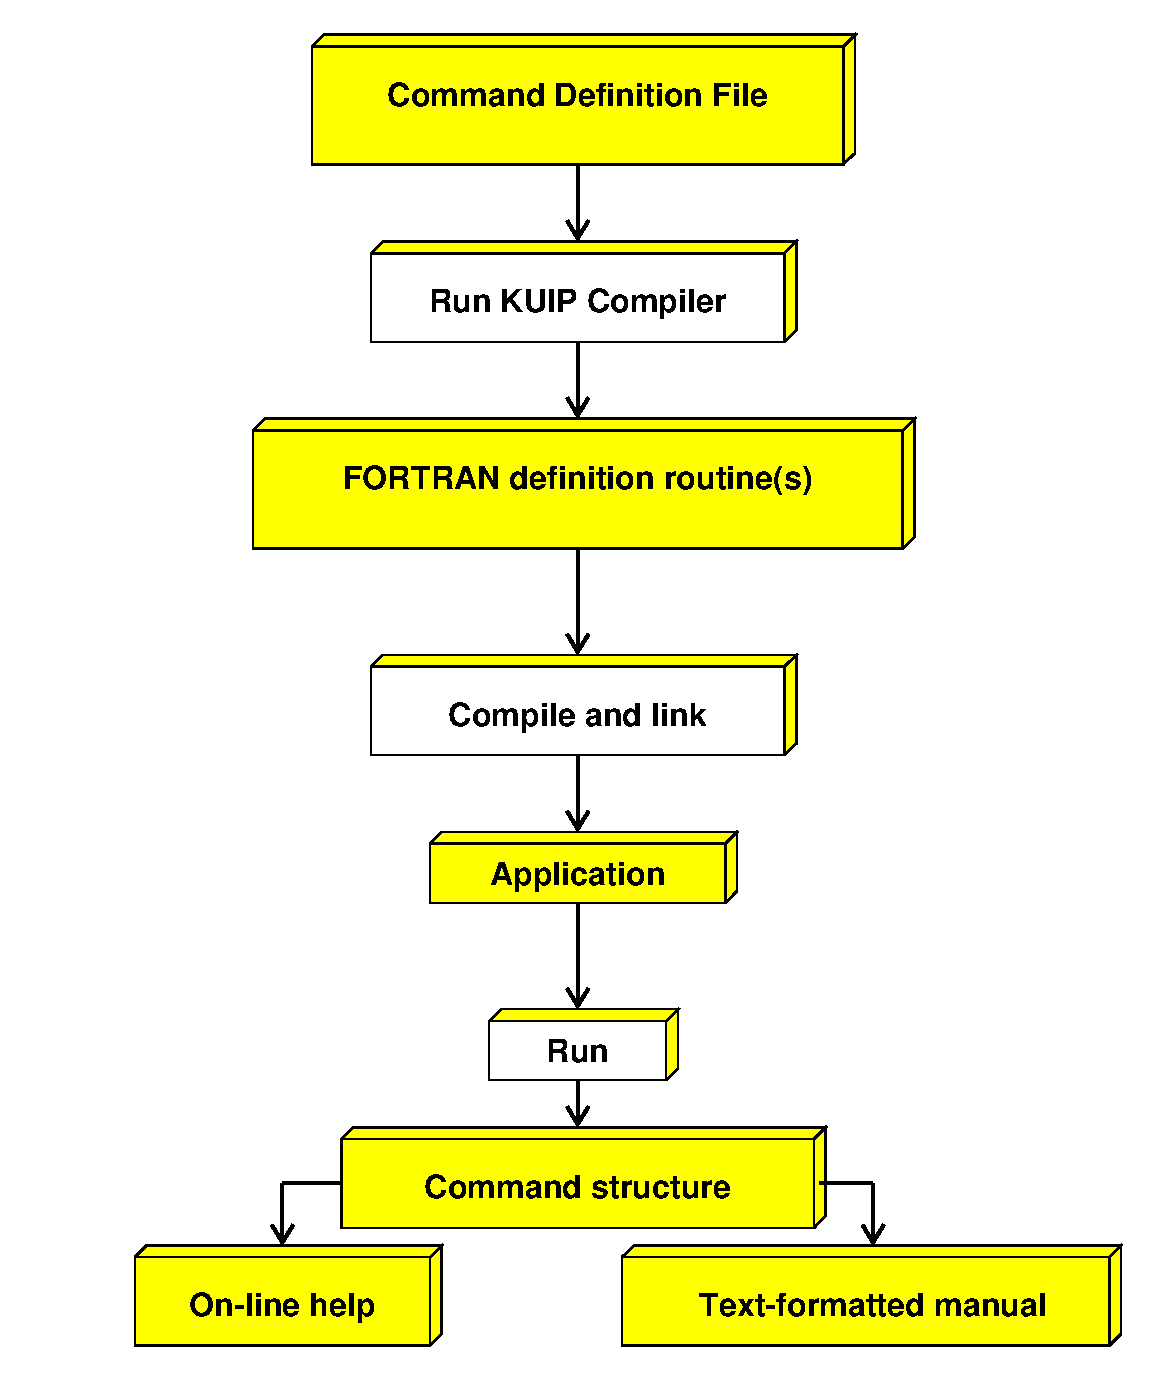
\epsfig{%bbllx=22mm,bblly=30mm,bburx=210mm,bbury=263mm,%
%              file=kuipc.eps,height=12cm}}
\end{center}
\caption{Building an application starting from the \CDF{}.}
\label{FIG8}
\end{figure}

\section{The Command Definition File}

The \CDF{} format is line-oriented.
Completely blank lines are ignored.
An underscore character at the end of a line acts as
continuation symbol, i.e.\ before processing
\index{CDF!continuation lines}
the following line is concatenated to the current line removing the
underscore itself.

Directives
\index{CDF!directives}
starts with a ``\Lit{>}''~character in the first column
immediately followed by the directive name.
Most directives take arguments following on the same line and some
directives expect additional information on separate lines.
\CDF{} argument lines are tokenized according to the rules:
\index{CDF!arguments}
\begin{UL}
\item
Individual arguments must be separated by one or more blanks.
\item
Strings containing blanks must be delimited by single quote characters,
e.g.\ \Lit{'Hello world'}.
\item
Single quote characters inside a string must be duplicated,
e.g.\ \Lit{'N''th value'}.
\item
A single ``\Lit{.}'' is the place-holder for a null argument.
\end{UL}

Names for menus, commands, and parameters
\index{Names}
are case-insensitive and may consists of letters,
digits, minus signs and underscores.
For obvious reasons names containing only digits, starting with a
minus sign, or ending in an underscore should be avoided.
Names may start with a digit.

\section{\CDF{} directives for command definitions\label{basic-CDF}}

The \CDF{} has to define the command tree structure which can contain
three types of elements: 
\begin{UL}

\item
Menus 
\index{menu!definition} 
are the branches of the tree.
Each menu should provide a help text to give general information
about the commands and sub-menus linked to it.

\item
Commands 
\index{command!definition} 
are the terminal leaves of the tree.
The \CDF{} should contain the help text and define the parameters 
(if any).
Each command definition must specify the action routine 
\index{action routine} 
which retrieves the command arguments and performs the intended operations.

\item
Help items \index{help item!definition} are like commands without
action routine. 
Their sole purpose is to provide additional help not related to a
specific command or menu.
Trying to execute a help item is equivalent to asking \Lit{HELP} on that item.

\end{UL}

\condbreak{5\baselineskip}
\begin{Gray}{i}
>* comment
   ...
\end{Gray}
\begin{Gray}{i}
*  comment
\end{Gray}
The \Lit{>*}~directive starts a block comment.
Everything up to the next \CDF{} directive is ignored.
A single line comment is introduced by a ``\Lit{*}''~character in the
first column. 


\begin{Gray}{i}
>NAME  definition-routine
\end{Gray}
The \Lit{>Name} directive defines the name of the routine which
\KUIPC{} will generate, i.e.\ \textsl{definition-routine} must be an acceptable
Fortran \Lit{SUBROUTINE} name.
The application has to \Lit{CALL }\textsl{definition-name} at initialization time
in order to store the command definitions in internal memory.


The first non-comment line in the \CDF{} must always be a \Lit{>Name}
directive. 
The \CDF{} may contain several \Lit{>Name} directives.

\begin{figure}[p]
\begin{XMPtext}{Example for the creation of menus}{
In this example \Lit{CALL KUIPDF} creates the menus \Lit{/KUIP},
\Lit{/KUIP/ALIAS}, \Lit{/KUIP/SET\_SHOW}, and \Lit{/MACRO} and 
\Lit{CALL VECDEF} creates the menu \Lit{/VECTOR}.
}
>Name KUIPDF
>Menu KUIP
>Guidance
      ...
>Menu ALIAS
>Guidance
      ...
>Menu ../SET_SHOW
>Guidance
      ...
>Menu /MACRO
>Guidance
      ...
>Name VECDEF
>Menu VECTOR
>Guidance
      ...
\end{XMPtext}
%\end{figure}
\vspace{-2\baselineskip}
%\begin{figure}[p]
\begin{XMPtext}{Example for the creation of commands}{
In this example the commands \Lit{/KUIP/HELP},
\Lit{/KUIP/ALIAS/CREATE}, and \Lit{/KUIP/ALIAS/DELETE} are created.
}
>Menu /KUIP
>Command HELP
      ...
>Menu ALIAS
>Command CREATE
      ...
>Command DELETE
      ...
\end{XMPtext}
%\end{figure}
\vspace{-2\baselineskip}
%\begin{figure}[p]
\begin{XMPtext}{Example for the creation of a help item}{
This example creates the help item \Lit{/KUIP/FUNCTIONS}.
}
>Menu /KUIP
>Help_item FUNCTIONS
>Guidance
      ...
\end{XMPtext}
\end{figure}

\begin{figure}[p]
\XMPvinput{Example for a guidance text}{xguidance.cdf}{}
\end{figure}

\begin{figure}[p]
\XMPvinput{Resulting HELP menu}{xguidance.hlp}{}
\XMPinput{Formatted output for ``MANUAL MYMENU -LATEX''}{xguidance.tex}{}
\end{figure}

\begin{figure}[p]
\XMPvinput{Example for a user help routine}{xuserhelp.f}{}
\XMPvinput{Terminal output for ``HELP MYMENU''}{xguidance.txt}{}
\end{figure}


\begin{Gray}{i}
>MENU  menu-path
\end{Gray}
Commands are linked into the current menu and the \Lit{>Menu}
directive allows to changes the menu path. 
The \textsl{menu-path} can consist of several components separated
by~``\Lit{/}''. 
The path is relative to the previously valid path unless \textsl{menu-path} starts with a~``\Lit{/}''.
The pseudo-name~``\Lit{..}'' refers to the parent menu.


The names for already existing menus may not be abbreviated.
If a menu is not already existing it is created and should be followed
by a \Lit{>Guidance} directive.

The \Lit{>Name} directive resets the path to the root
menu~``\Lit{/}''. 
Commands and help item should not be linked directly to the root menu.
Therefore the \Lit{>Name} directive should always be a followed by a
\Lit{>Menu} directive. 


\begin{Gray}{i}
>COMMAND  command-name
\end{Gray}
The \Lit{>Command} directive appends a new command to the
current menu.
The \textsl{command-name} must be a bare name without menu path.

The \Lit{>Command} directive must be followed by \Lit{>Guidance} and
\Lit{>Action} directives and can be followed by \Lit{>Parameters} and
\Lit{>User_help} directives in any order.


\begin{Gray}{i}
>HELP_ITEM  help-item-name
\end{Gray}
The \Lit{>Help_item} directive appends a new help item to the
current menu.
The \textsl{help-item-name} must be a bare name without menu path.
The \textsl{help-item-name} cannot contain a menu path.

The \Lit{>Help_item} directive must be followed by a \Lit{>Guidance}
directive and can be followed by a \Lit{>User_help} directive in any order.

\condbreak{2cm}
\begin{Gray}{i}
>GUIDANCE
   text
   ...
\end{Gray}
The \Lit{>Guidance} directive defines the help text attached to the
most recent command tree element created by a \Lit{>Menu},
\Lit{>Command}, or \Lit{>Help\_item} directive.
The help text ends at the next \CDF{} directive.
The formatting rules applied for terminal output and by the 
\Lit{MANUAL} command in \LaTeX{} mode are explained in the example below.


\begin{Gray}{i}
>USER_HELP  user-help-routine
\end{Gray}
The \Lit{>User_help} directive may follow a \Lit{>Command} or
\Lit{>Help_item} directive.
The \textsl{user-help-routine} is called by the \Lit{HELP} command and
allows to add runtime dependent information at the end of the static
\Lit{>Guidance} text. 

The routine has to call \Lit{KUHELP} in order to obtain the 
logical unit where the additional help information should be written to.
The second argument of \Lit{KUHELP} returns the command or help item
name for which \Lit{HELP} was requested.

\begin{Gray}{i}
>PARAMETERS
  mandatory-parameters
+
  optional-parameters
++
  constant-parameters
\end{Gray}
The \Lit{>Parameters} directive heads the parameter definition for a command.
The lines following up to the next directive must be parameter
definitions of the form

\indent\indent\begin{tabular}{llll}
\textsl{parameter-name} & \textsl{prompt-string} & \textsl{parameter-type}
& $[$ \textsl{attribute-list} $]$
\end{tabular}
\vskip\parskip

The underscore continuation has to be used if the complete definition
does not fit onto a single single.
Mandatory and optional parameters are separated by a control line
containing only a ``\Lit{+}''~character in the first column.
If there are only mandatory parameters the ``\Lit{+}''~line is not
required.


Non-positional arguments can be specified
in a command line as \textsl{parameter-name}{\tt=}\textsl{value}.
To allow abbreviations for \textsl{parameter-name} the minimum length has
to be indicated by a ``\Lit{*}''~character, e.g.\
\begin{XMP}
DIR*ECTORY \quad 'Directory path' \quad C
\end{XMP}
defines a parameter \Lit{DIRECTORY} which can be assigned in a command
line as ``\Lit{DIR=}\textsl{value}''.

The \textsl{prompt-string} is used to prompt for missing mandatory
arguments and as labels in the \Motif{} command panel.
Possible \textsl{parameter-type} values are ``\Lit{C}''~for character
strings, ``\Lit{I}''~for integer numbers, and ``\Lit{R}''~for real
numbers.

The \textsl{attribute-list} for mandatory parameters can be empty.
For optional parameters it must specify at least the default attribute:
\begin{XMP} 
D=\textsl{default-value}
\end{XMP}
For mandatory parameters the default value is only used when prompting
for missing arguments and the reply is an empty line.
The default value for optional parameters is passed to the action
routine whenever the argument is missing or given as~``\Lit{!}'' on
the command line.

For all parameter types~\Lit{C}, \Lit{I}, and~\Lit{R} the range
attribute defines a comma-separated list of valid values:
\begin{XMP} 
R=\textsl{value-1},\textsl{value-2},...\textsl{value-n}
\end{XMP}
e.g.\
\begin{XMP} 
PRIME \quad 'Prime number below 10' \quad I \quad R=2,3,5,7
\end{XMP}
For option parameters there is an alternative way to specify the list
of valid values together with an explanation text for each option (see below).
For the numeric parameter types~\Lit{I} and~\Lit{R} the range
attribute can have the form
\begin{XMP} 
R=\textsl{lower-limit}:\textsl{upper-limit}
\end{XMP}
to limit valid values to the interval including the boundaries.
Either the \textsl{lower-limit} or the \textsl{upper-limit} may be
omitted to indicate an unlimited interval in one direction.

Numeric parameters with a limited range are displayed with a slider in
the \Motif{} command panel.
The slider step size for type~``\Lit{R}'' parameters is determined by
the number of digits following the decimal point in the range
definition, e.g.\
\begin{XMP} 
PROB*ABILITY  'Detection probability'  R  D=0.5  R=0:1.00
\end{XMP}
creates a slider for the values 0.00, 0.01, ..., 1.00.
If the range is unlimited or too large the \Lit{Slider} attribute
\begin{XMP} 
SLIDER=\textsl{lower-limit}:\textsl{upper-limit}
\end{XMP}
allows to define a restricted range which affects the slider only.
E.g.\
\begin{XMP} 
EFF*ICIENCY  'Reconstruction efficiency'  R  R=0:1  Slider=0.900:1
\end{XMP}
creates a slider for the values 0.900, 0.901, ..., 1.000.

\begin{figure}[tb]
\XMPvinput{Example for option parameter definitions}{xparameter.cdf}{}
\end{figure}

\begin{figure}[tb]
\XMPvinput{Argument assignments for command ECHO}{xparameter.log}{}
\end{figure}

%\begin{figure}[tb]
%\XMPvinput{Terminal output for ``HELP ECHO''}{xparameter.txt}{}
%\XMPinput{Formatted output for ``MANUAL ECHO -LATEX''}{xparameter.tex}{}
%\end{figure}

The \Lit{Option} attributes defines a parameter to be an option for
which ``\Lit{-}\textsl{value}'' can be used to specify non-positional
option arguments on the command line.
The \Lit{Option} attribute is set implicitly
if \textsl{parameter-name} begins with \Lit{OPTION} or \Lit{CHOPT}.
The ``\Lit{-}''~mechanism requires a range definition including all
valid option values.
The list of option values is defined by lines
\begin{XMP} 
-\textsl{option-value} \quad \textsl{explanation-text}
\end{XMP}
following the option parameter definition itself.
The ``\Lit{-}''~character must be in the first column and is not part
of the option value.
The underscore continuation has to be used if the complete 
\textsl{explanation-text} does not fit onto a single single.
The rules applied for formatting the list of options as a table are
explained in the example. 

A command can contain contain several option parameters as long as the
option values are distinct.
Option values can be specified with the range attribute
if an \textsl{explanation-text} is not required.
Blank is permitted as \textsl{option-value} but cannot be combined with
any other value.
Consequently it should only be used if all option values are mutually
exclusive, and it should be the default value.

The interpretation of a ``\Lit{-}\textsl{value}'' argument as option
is considered only if \textsl{value} consists
exclusively of valid values from a single option parameter.
In some instances ``\Lit{-}\textsl{value}'' is intended be a positional
argument even though it could match an option parameter as well.
It depends then on the definition of the parameter which
should be assigned next whether the argument is actually interpreted
as option ``\textsl{value}''.

If ``\Lit{-}\textsl{value}'' can be interpreted as a negative number
and the next parameter is numeric the option assignment is inhibited.
A character parameter can be given the \Lit{Minus} attribute to
indicate that arguments at its position should never be assign to an
option parameter.

The leading ``\Lit{-}'' is usually stripped off in an option
assignment. 
Only in case the next argument position belongs to the option
parameter itself and ``\Lit{-}'' is one of its option values
it is passed on to the action routine.
In order to avoid confusion due to this position dependence digits and
the minus sign should not be used as option values.


It is often desirable for a command to be able to accept a
variable-length list of values for one of the parameters.
If the command operation is independent for each list item
the \Lit{Loop} attribute can be added to the corresponding parameter
definition.
For a comma-separated argument list the action routine is then called
repeatedly passing it the next list item each time.
E.g.\ with the definition
\condbreak{1cm}
\begin{XMP}
>Command DELETE
>Parameters
LIST  'List of items'  C \quad Loop
\end{XMP}
the command line
\begin{XMP}
DELETE x,y,z
\end{XMP}
is equivalent to
\begin{XMP}
DELETE x ;  DELETE y ;  DELETE z
\end{XMP}
and the action routine only needs to handle a single item.
A ``\Lit{,}'' inside a quoted string or an unbalanced set of
parentheses is not treated as item separator, i.e.\ ``\Lit{'foo,bar'}''
and ``\Lit{xyz(3,4,5)}'' are single items only.

In case the action routine needs access to all list items it can call
\Rind{KUGETL} to retrieve the items one by one.
The \Lit{Vararg} attribute can be given to a list parameter if it is
the last one of the command. 
This allows to use \Rind{KUGETL} also for a blank separated item list,
i.e.\ with the definition
\begin{XMP}
>Command ASSIGN 
>Parameters 
ARRAY  'Array name'  C 
VALUES  'List of values'  C  Vararg
\end{XMP}
both command line forms
\begin{XMP}
ASSIGN  name  foo,bar 
ASSIGN  name  foo  bar
\end{XMP}
can be handled by the same action routine.

In \Motif{} mode the arguments entered in the command panel are usually
treated as a single value, i.e.\ if they contain a blanks they are
implicitly quoted.
In some cases, for example the macro arguments passed in the
\Cind{EXEC} command, this behavior must be inhibited.
The \Lit{Separate} attribute allows to flag the last parameter that
the value entered in the \Motif{} input field should be interpreted as
separate command line tokens.


\condbreak{3\baselineskip}
\begin{Gray}{i}
>ACTION  action-routine
\end{Gray}
The \Lit{>Action} directive must follow a \Lit{>Command} and defines
the routine which should be called after decoding the command line in
order to perform the intended operations.

\begin{figure}[tb]
\XMPvinput{Example for an action routine}{xecho.f}{}
\end{figure}

An action routine does not have arguments.
The command line arguments have to be retrieved 
by calling the suitable \Lit{KUGET}\textsl{x} routine for each parameter
from inside the action routine.

The same action routine can be used for different commands.
The routines \Lit{KUPATH} and \Lit{KUPATL} allow to identify which
command was actually requested.

\if0
\section{Retrieving parameters in action routines}

Action routines are called automatically by \KUIP{} when the corresponding
command is entered. The application programmer, in addition to defining
their names with the \Command{>Action} keyword in the \CDF{}, will have to write
these action routines and to link them together with the rest of its application.

Inside action routines, parameters, as defined with \Command{>Parameters}
in the \CDF{}, have to be retrieved by calling the
\KUGETx{} routines, e.g.:
\Rind[KUGETI]{KUGETI(IPAR)}, \Rind[KUGETR]{KUGETR(RPAR)}, 
\Rind[KUGETC]{KUGETC(CHPAR,NCH)},\ldots for parameters of the
type Integer, Real and Character type parameters respectively.
%
%---------------------------------------------------------------------------
%
\fi
%
%---------------------------------------------------------------------------
%
\section{Browser Concepts and Definitions}
\label{ref:rebrodef}

The high-light of the \KUIPMotif{} interface is a general-purpose object
browser.
Before going into the details of the \CDF{} directives for customizing
the browser we want to introduce the main concepts and the terminology
used.

The browser allows to traverse a hierarchical directory structure of 
objects. Operations on these objects can be chosen from pop-up menus which
depend on the object type (or ``class'').

To incorporate your own application specific objects into the browser
you have to:
\begin{UL}
\item
describe in the \CDF{} (``Command Definition File'') the object types 
(``classes'') and the containers for these objects (``browsables''),
\item
write ``small'' routines to scan through the list of objects, and 
eventually the list of browsables,
\item
describe in the \CDF{} the action menus for classes of objects and browsables.
\end{UL}

\subsection{Classes of Objects}
\label{ref:recldef}

``Classes'' of objects can be any kind of entities handled by an application.

For example:
\begin{UL}
\item
HIGZ pictures and \HBOOK{} data (1d-histograms, 2d-histograms, 
N-tuples, chains and directories) are ``Classes'' defined in
\PAW++{}.
\item
in Geant++  the classes are the data structures: volumes, materials, 
particles, ...
\item
in \KUIPMotif{} the commands themselves have been defined as classes,
as well as the different type of files (read, read-write, executable,
and macros ...).
\end{UL}

Object classes are defined in the \CDF{} with the directive:
\begin{Gray}{i}
>Class  class-name  menu-title  [ big-icon  small-icon ]
\end{Gray}

\begin{figure}[tb]
\begin{PICTf}[.45]{pkmf15}
\begin{DLsf}{}
\item[\quad \CDF{} description (extract) :]
\item
\item
\begin{XMPt}{Example of the ``Class'' directive}\footnotesize

>Class 1d 1d-Histogram big_1d sm_1d
 Plot        .  .  default_action%C
'/Fit...'    .  'Histo/Fit [this]'
'Fit Gauss'  .  'Histo/Fit [this] G'
'Fit Exp'    .  'Histo/Fit [this] E'
'Fit Const'  .  'Histo/Fit [this] P0'
'Fit Linear' .  'Histo/Fit [this] P1'
 /Smooth     .  'Smooth [this]'
'Smooth...'  .  '-Smooth [this]'
 /Copy       .  'Histo/Copy [this]'
 Reset       .  'Histo/Op/Reset [this]'
!Delete      .  'Hio/Hscratch [this]'
+
...
\end{XMPt}
\end{DLsf}
\end{PICTf}
\begin{EnumZB}
\item Icon used to represent the object class ``1d'' (normal size).
\item Action menu (title ``1d-Histogram'') associated to the selected object 
(histogram of class ``1d'' with name/identifier ``10'').
\vspace{-1\baselineskip}
\end{EnumZB}
\caption{Object Classes}
\label{ref:FIGPKMF15}
\end{figure}

E.g.\ The directive ``{\tt >Class 1d '1d-Histogram' big\_1d sm\_1d}'' in the 
\PAW{} \CDF{} is used for 1D histograms : the class name is ``1d'', ``big\_1d''
(normal size) and ``sm\_1d'' (small size) are the icons used by the browser 
for a graphical representation and ``1d-Histogram'' is the title text for
the pop-up menu displayed when object types ``1d'' are selected in the browser
(see figure~\ref{ref:FIGPKMF15}).

\subsection{Browsables}
\label{ref:rebrdef}

All objects are part of container objects constituting the top level directory
(e.g.\ ZEBRA/RZ files.). We will call these containers the ``browsables''.
They are defined with the \CDF{} directive
\begin{Gray}{i}
>Browse  browsable-class  menu-title  scan-objects  [ scan-browsables ]
\end{Gray}

\begin{figure}[tb]
\begin{PICTf}[.5]{pkmf16}
\begin{DLsf}{}
\item[\quad \CDF{} description (extract) :]
\item
\item
\begin{XMPt}{Example of the ``Browse'' directive}\footnotesize

>Browse Commands . kscncmds%C
 List
'Set Default'  .  ' Set/Root /'
...
>Class /Menu Menu big_menu sm_menu
...
>Class Cmd Command big_cmd sm_cmd
...
\end{XMPt}
\end{DLsf}
\end{PICTf}
\begin{EnumZB}
\item The browsable ``Commands'' is selected.
\item Action menu corresponding to this browsable.
\item \OW{} with the list of commands (class ``Cmd'') and menus 
(class ``/Menu'') for the current directory ``/KUIP'' \NbDB{4}.
\vspace{-1\baselineskip}
\end{EnumZB}
\caption{Browsables}
\label{ref:FIGPKMF16}
\end{figure}

For example:
\begin{UL}
\item
in \PAW++{}, a browsable HBOOK (see figure~\ref{ref:FIGPKMF16}) has been
defined, which is a container for any  
kind of \HBOOK{} data (1d/2d histograms and Ntuples).
\item
in \KUIPMotif{}, the browsable ``Files'' contains and displays all files
(read, read-write, executables, and \KUIP{} macros). Another browsable 
``Commands'' has been defined for all the commands and menus defined 
by \KUIP{} and the application.
\end{UL}

For a detailed description of the ``{\tt >Class}'' and
``{\tt >Browse}'' \CDF{} directives see sections~\ref{ref:recdfobj} 
and~\ref{ref:recdfbro}.

\subsection{The ``scan-objects'' routine}

To make the objects belonging to one browsable for a given path (directory)
accessible by the browser, the application has to provide a scanning routine 
which, when called for the first time, returns the first object and
subsequently returns the next object until no more objects are left: this
is what we have called the ``scan-objects'' routine in the \CDF{} directive 
for the browsable definition. The browser passes to this routine the 
identification of the requested subdirectory and expects in return:
\begin{UL}
\item
the object name, e.g.: 
\begin{UL}
\item
for ``{\tt >Browse HBOOK}'' in \PAW++{}: the histogram or Ntuple identifier 
(number).
\item
for ``{\tt >Browse Commands}'' in \KUIPMotif{}: the menu or command name.
\end{UL}
\item
the object class, e.g.: 
\begin{UL}
\item
for ``{\tt >Browse HBOOK}'' in \PAW++{}: ``1d'', ``2d'' or ``Ntuple'' 
(assuming that ``{\tt >Class 1d}'', ``{\tt >Class 2d}'' and 
``{\tt >Class Ntuple}'' have been defined).
\item
for ``{\tt >Browse Commands}'' in \KUIPMotif{}: ``Menu'', ``Cmd'' and ``InvCmd''
(assuming that ``{\tt >Class Menu}'', ``{\tt >Class Cmd}'' and 
``{\tt >Class InvCmd}'' have been defined).
\end{UL}
\item
and eventually a short and a long description text (title) of this object 
(which will be used to display the list of objects in various forms: big icons, 
small icons, text only).
\end{UL}
This ``scan-objects'' routine can be coded in Fortran or in~C. 

\subsection{The ``scan-browsables'' routine}

We have to make a distinction between two kinds of browsables:
\begin{UL}
\item
``single instance'' browsables,
\item
or ``multiple instances'' browsables.
\end{UL}
A ``multiple instances'' browsable gives the possibility to have several
instances of the same browsable. For instance, in \PAW++{}, the browsable
``{\tt >Browse HBOOK}'' which is defined for the ZEBRA/RZ files, acts as a
container for the objects 1d/2d histograms and Ntuples. As it is
possible to have several ZEBRA/RZ files opened at the same time and 
connected to different logical units (LUN), the browsable HBOOK has been
defined as a ``multiple instances'' one. This is done by providing
a second scanning routine from which the name of all the currently connected
instances of a given browsable can be retrieved (e.g.\ for all the ZEBRA/RZ 
files opened and connected to some logical unit  the name is a concatenation
of ``LUN'' and this number, i.e.\ ``LUN8'' for logical unit 8).
This is what we have called the ``scan-browsables'' routine  (optional for a 
``single instance'' browsable) in the \CDF{} directive for the browsable 
definition.

This ``scan-browsables'' routine can be coded in Fortran or in~C.

Note that ``single instance'' browsables are always displayed in the 
browser (as soon as it is created) whereas ``multiple instances''browsables
can be accessed and displayed at run time (e.g.\ in \PAW++{} when a new 
ZEBRA/RZ file is opened).

For a more precise description of the the calling sequence of the 
``scan-objects'' and ``scan-browsables'' routines see section 
\ref{ref:recdfbro}.

\subsection{Directories}

A tree structure of objects can easily be achieved by defining a special class
for subdirectories of a browsable. The corresponding \CDF{} directive 
is the same 
as for simple object classes, ``{\tt >Class}'', except that there must a 
``{\tt /}'' in front of the class name.

For example:
\begin{UL}
\item
in \PAW++{}, ZEBRA/RZ directories (browsable ``HBOOK'') are ``directories''
classes of objects: 
\begin{XMPt} {}
       >Class /dir Directory big\_dir sm\_dir
\end{XMPt}
Ntuple chains (in the ``Chains'' browsable) are also defined as a ``directory'' 
class of objects:
\begin{XMPt} {}
       >Class /chain Chain big\_chain sm\_chain
\end{XMPt}
\item
in \KUIPMotif{} the menus (in the ``Commands'' browsable) are defined as 
a ``directory'' class of objects:
\begin{XMPt} {}
       >Class /Menu Menu big\_menu sm\_menu
\end{XMPt}
This is also true for directories of files (in the ``File'' browsable):
\begin{XMPt} {}
       >Class /DirFile Directory big\_menu sm\_menu
\end{XMPt}
\end{UL}

This ``special'' class of objects obeys to certain rules:
\begin{UL}
\item
The first item in the action menu is always ``List'' and means ``switch into 
this subdirectory''. Selecting this item (automatically performed with 
a <double click> with the left button) has the effect to update
the content of the \OW{} with the list of objects contained
into the new subdirectory.
\item
The entry ``Path:'' (Fig. \ref{ref:FIGPKMF16}, 
\NbDB{4}) is automatically updated
with the new directory path, which is formed by concatenating the previous
path, a ``{\tt /}'', and the name of the directory object selected.
Going upwards in the directory hierarchy is done by selecting a
substring of the current path displayed in this text entry. Clicking
a second time on the same path segment performs the directory change
and updates the \OW{} in the same way as selecting the ``List'' 
menu entry for a directory object.
\end{UL}

\subsection{Action menus}

For each class of objects it is possible to define two menus which describe 
possible actions if an object of this class is selected:
\begin{UL}
\item[(1)]
either in the browser \OW{},
\item[(2)]
or identified inside a HIGZ \GW{} (if any).
\end{UL}

\condbreak{3\baselineskip}
For each browsable it is possible to define:
\begin{UL}
\item[(3)]
one menu which describes possible 
actions if this browsable is selected (\BW{}), 
\item[(4)]
for ``multiple instances'' browsables, a second menu which describes 
the actions required to connect or de-connect one instance of this 
browsable at run time (menu ``File'' in the \MB{}).
\end{UL}

Menus (1), (2) and (3) pop up when pressing the right mouse button 
in the corresponding window, and the
selected action is performed when the button is released. A <double click>
with the left mouse button on one specific object or on one specific 
browsable always executes the first menu item. Menu (4) is accessed by 
selecting the entry ``File'' in the \MB{} menu-bar.

Object and browsable specific action menus are derived from sequences of action 
definitions written in the \CDF{} and following the {\tt >Class} or 
{\tt >Browse} directive (Fig. \ref{ref:FIGPKMF15} and \ref{ref:FIGPKMF16}). 
For a precise description of the syntax and behavior 
of the \CDF{} directives for action menus see section \ref{ref:recdfacm}.


\section{\CDF{} directives for \KUIPMotif{}\label{Motif-CDF}}

\label{ref:recdf}

We will describe in this section the new \CDF{} (Command Definition File)
directives which have been introduced in \KUIPMotif{}. Please note that
these new directives have to be used only to take advantage of the MOTIF
style and to include your application specific objects into the interface
(and especially into the browser(s)). BUT one must be aware that IT IS 
POSSIBLE to get a \Motif{} interface for any \KUIP{} based application 
WITHOUT modifying the \CDF{}, but only modifying very slightly the 
application main program in order to give control to the ``\Motif{} main loop'' 
(i.e.\ call KUWHAM instead of KUWHAT or KUWHAG).

In all the directives we will describe the square brackets (``[]'') mean
that the corresponding entity is optional: either some default value
is automatically provided if it is missing (e.g.\ for titles), or the
entity is not necessary requested. If such an optional entity happens
to be in the middle of the directive (not at the end) then it has
to be replaced by a ``.'' if no real value is given.

We advice users who want to take advantage of the \Motif{} style to compile 
their \CDF{}s into C~code (instead of Fortran): this is automatically 
performed by the \KUIPC{} compiler when giving the extension ``\Lit{.c}'' to the 
output file which is produced.

N.B. It is preferable to separate the directives for the usual command mode
interface and the directives specific to the \Motif{} style (objects, browsables
and action menus definitions) into different \CDF{}s. Then it will be easy
and possible to make the same application work on a dumb terminal (offering 
only the \KUIP{} command mode interface) or on a \Motif{} workstation, with only 
very few differences in the application main program. 

\subsection{For Classes of Objects}
\label{ref:recdfobj}

As we have already seen (section \ref{ref:recldef}), classes of objects 
are defined in the \CDF{} with the directive
\begin{Gray}{i}
>Class  class-name  menu-title  [ big-icon  small-icon ]
\end{Gray}
for example,
\begin{XMP}
>Class ExFile 'Executable File' big_fx sm_fx
\end{XMP}

The ``menu-title'' should be a short explanation concerning the class (or type)
of object and is used as a title text for the action menu which is displayed
when one object of this class is selected (either in the browser, or in the
\GW{} if any). If no title is given the ``class-name'' is used 
instead. 

``big-icon'' and ``small-icon'' are the names for the icons representing 
graphically this class of object inside the browser. Default icons are
provided if these values are missing, but then the same iconic representation
will be used for all object classes. It is a lot better to have a different
representation for each object class. To create a new icon bitmap you can use
the X11 standard bitmap editor. The icons definitions in the \CDF{} follow
the directive {\tt >Icon\_bitmaps} (see \ref{ref:rebmdef}).


\subsection{For Browsables}
\label{ref:recdfbro}

As we have seen in section \ref{ref:rebrdef}, browsables are defined with the 
\CDF{} directive
\begin{Gray}{i}
>Browse  browsable-class  menu-title  scan-objects  [ scan-browsables ]
\end{Gray}
for example,
\begin{XMP}
>Browse Macro . kmbmac%C kmbmdi%C
\end{XMP}

The ``menu-title'' should be a short explanation on the browsable itself
and is used as a title text for the action menu which is displayed
in the browser ``FileList'' window when this browsable is selected. If a 
``.'' is put instead, then the browsable-class becomes by default the 
menu-title.

\subsubsection{The ``scan-objects'' Routine}
\label{ref:recdfsco}

The ``scan-objects'' routine can be written in Fortran or in~C. 
The browser passes to this routine the identification of the requested 
subdirectory (path) and expects in return: the object name, the class 
name, and eventually a short and a long description text (title) of this 
object. In both cases (Fortran or~C) the calling sequence is predefined. 

In Fortran the calling sequence of the ``scan-objects'' routine 
is the following:
\condbreak{3cm}
\begin{XMPt}{scan-objects routine (in Fortran)}\footnotesize
      SUBROUTINE SCNOBJ(BRNAME,BRCLAS,BRPATH,OBNAME,OBCLAS,STEXT,LTEXT)
      CHARACTER*(*) BRNAME,BRCLAS,BRPATH,OBNAME,OBCLAS,STEXT,LTEXT
*
*            Browser interface to return next object
*
*            Input Parameters  :
*
*                      BRNAME  : browsable name (displayed in the browser)
*                      BRCLAS  : browsable class name (from the ``>Browse'' directive)
*                      BRPATH  : current directory path
*
*            Input / Output    :
*
*                      OBNAME  : object name or identifier
*                                ' ' the first time, previous object otherwise
*
*            Output Parameters :
*
*                      OBCLASS : class name                
*                      STEXT   : short text description of the object
*                      LTEXT   : long text description of the object
*
*     ...
*     IF(OBNAME.EQ.' ') THEN
*        Initialize the scan-objects routine        
*     ENDIF
*     ...
*
      OBCLASS = ...
      STEXT = ...
      LTEXT = ...
*
      END
\end{XMPt}

\condbreak{4cm}

In C the calling sequence is:
\begin{XMPt} {scan-objects routine (in C)}
char **scnobj( brobj_name, brcls_name, bpath, n )
     char *brobj_name;  /* browsable name (displayed in the browser) */
     char *brcls_name;  /* browsable class (from the ``>Browse'' directive) */
     char *bpath;       /* current directory path */
     int n;             /* object position (0 the first time) */
\{
  static char     *obj_desc[4];

    ...
    if (n == 0) \{
       /* Initialize the scan-objects routine */
    \}
    ...

    return obj_desc;   /* obj_desc[0] --> object name or identifier
                          obj_desc[1] --> class name
                          obj_desc[2] --> short text description of the object
                          obj_desc[3] --> long text description of the object
                        */
\}
\end{XMPt}

The browsable name and class-name are identical for ``single instance'' 
browsables. They can be different for ``multiple instances'' browsables.
e.g.\ for ``{\tt >Browse HBOOK}'' in \PAW++{}: the browsable class is ``HBOOK'' 
and the browsable name is ``LUN8'' for a ZEBRA/RZ file connected to logical 
unit 8.

The selected object name (or identifier) and its corresponding long text 
description are printed at the very bottom line of the browser
(\NbDB{6} in Fig.\ref{ref:FIGPKMF9}).

\subsubsection{The ``scan-browsables'' Routine}
\label{ref:recdfscb}

The ``scan-browsables'' routine (optional for ``single instance'' browsables 
but required for ``multiple instances'' ones) can be written in Fortran or 
in~C.  The browser passes to this routine the browsable class-name (e.g.\ 
in \PAW++{}, ``\Lit{HBOOK}'' for ZEBRA/RZ files) and expects in return: the browsable 
name (e.g.\  ``\Lit{LUN8}'' for a ZEBRA/RZ file connected to logical unit~8)
and eventually a string with the description of a predefined set of 
variables concerning this browsable. These variables are used as ``key-words''
in the actions menus connected to the browsables or the classes of objects. 
Some of these variables are fixed by \KUIPMotif{} itself:
\begin{UL}
\item
the variable ``file'' is used to fill the corresponding label (``File:'') 
at the bottom of the browser. 
\item
``root'' is used for setting the path of the top level directory 
(e.g.\ ``\Lit{//LUN8}''),
\end{UL}
The `scan-browsables'' routine for a ``single instance'' browsable can be 
defined just for setting this ``description string'' with the required
key-words.

\condbreak{4cm}

In Fortran the calling sequence of the ``scan-browsables'' routine 
is the following:
\begin{XMPt}{scan-browsables routine (in Fortran)}\footnotesize
      SUBROUTINE SCNBRO(BRCLAS,BRNAME,VARSET)
      CHARACTER*(*) BRCLAS,BRNAME,VARSET
*
*            Browser interface to return next browsable instance
*
*            Input Parameters  :
*
*                      BRCLAS  : browsable class name (from the ``>Browse'' directive)
*
*            Input / Output    :
*
*                      BRNAME  : browsable name (displayed in the browser)
*                                ' ' the first time.
*
*            Output Parameters :
*
*                      VARSET  : set of variables for this browsable.
*
*     First call to this routine 
      IF(BRNAME.EQ.' ') ...
*
      ... 
\condbreak{7\baselineskip}\vspace{-\baselineskip}
      BRNAME = ...
      VARSET='root= ... file= ... ...=...'
      ...
*
      END
\end{XMPt}
E.g.\ in \PAW++{}, for ``{\tt >Browse HBOOK}'' and the browsable ``LUN8'' (ZEBRA/RZ
file connected on logical unit 8) the routine SCNBRO will return something
like:
\begin{XMP}
VARSET = root=//LUN8 file='/user/paw/demo/hrztest.dat'  unit=8
\end{XMP}
In this example ``unit'' is a key-word specific to the browsable HBOOK that 
can be used later on in the action menu definition (e.g.\ ``Close [unit]'').
(See next section \ref{ref:recdfacm} for a complete description of the 
``action menu definition'').

\condbreak{4cm}
In C the calling sequence is the following:
\begin{XMPt} {scan-browsables routine (in C)}
char **scnbro( class_name, first )
     char *class_name;
     int first;
\{
    static char *path_desc[2];

    ...
    if (first) {
       /* First call to this routine */
    }
    ...

    return path_desc;  /* path_desc[0] --> browsable name
                          path_desc[1] --> set of variables for this browsable
                        */
\}
\end{XMPt}

\subsection{For Actions Menus}
\label{ref:recdfacm}

Both the ``{\tt >Class}'' and ``{\tt >Browse}'' directives can be followed 
by sequences of action definitions which obey to the following syntax:
\begin{Gray}{i}
menu-text  [ special-flags ]  [ action-string ]  [ action-routine ]
\end{Gray}
N.B. the components which are missing, when optional (enclosed with ``[]'' 
in the syntax description above), must be replaced by a ``.'' if they are
not the last ones.

The ``menu-text'' is the text that will appear in the pop-up menu. It should
be short but meaningful. ``/'' and ``!'', when they are the very first 
character of this menu-text have special meanings:
\begin{UL}
\item
a ``/'' means that the menu item has to be preceded by a separator,
\item
a ``!'' means that the browser has to be updated when the action is
performed (because the ``objects window'' may have changed).
\end{UL}

The entity ``special-flags'' is not used at the moment and has to be
replaced by a ``.''.

The action can be specified as a string of commands (``{\tt action-string}'')
which should be executed and/or a user-written and application specific 
routine (``{\tt action-routine}'') which should be called. 

In both cases (``{\tt >Class}'' and ``{\tt >Browse}'') two sets of menus 
can coexist and are separated by a blank line starting with the 
character ``+''. The first menu always applies to objects/browsables 
which are identified in the browser. In most cases the
menu pops up when pressing the right mouse button and the selected
action is performed when the button is released.

For the ``{\tt >Class}'' directive the second menu applies to objects which 
are identified in the HIGZ \GW{} if any. (E.g.\ in \PAW++{}, 
``{\tt >Class 1d}'' and ``{\tt >Class 2d}'' histograms can be 
identified either in the browser or in the graphics window: two sets of
menu are then defined in the \CDF{}). 

For the ``{\tt >Browse}'' directive a second menu can be defined to fill 
the ``File'' menu-bar entry in the browser with the list of commands to 
connect or de-connect one instance of a ``multiple instances'' browsable 
(e.g.\ in \PAW++{} open or close a ZEBRA/RZ file containing \HBOOK{} data). 

Only one of the two menu sets can be defined in both cases.

N.B. For graphical object identification inside the graphics window 
please refer to the description of the two HIGZ routines \IGPID{} and
\IGOBJ{} in the HIGZ manual \cite{bib-HIGZ}.

\subsubsection{Action-string (String of Commands)}

When the action is specified as a string of commands,
constructs of the form ``{\tt [}{\em var}{\tt ]}'' can insert
identifications of the selected object in the command string:
\begin{UL}
\item
{\tt [this]} is replaced by the object name, e.g.\ in \PAW++{}: histogram ``10''.
\item
{\tt [that]} is replaced by the short description text returned by the
scanning routine and can thus be used as an alias name.
\item
{\tt [name]} is replaced by the name of the browsable,
e.g.\ in \PAW++{}, ``{\tt LUN8}'' for an ZEBRA/RZ file opened on unit~8.
\item
{\tt [root]} is replaced by the path of the top level directory,
e.g.\ in \PAW++{}, ``{\tt //LUN8}''.
\item
{\tt [path]} is replaced by the complete path to the directory in which the
object is contained, e.g.\ in \PAW++{}, ``{\tt //LUN8/MYDIR}''.
Initially, {\tt [path]} is set to {\tt [root]}.
\end{UL}

As we have seen in the previous section (\ref{ref:recdfscb}) the replacement
values for {\tt [name]}, {\tt [root]} and, eventually, additional 
variables specific to the application (e.g.\ {\tt [unit]} in \PAW++{} for
the browsable HBOOK) have to be returned by the application specific
``scan-browsables'' routine. For single instance
browsables, when this routine (optional) is not defined, {\tt [name]} is 
substituted by the class name and the field {\em menu-title} of the 
{\tt >Browse} directive is used as the definition of {\tt [root]}.


\subsubsection{Action-routine}

If the action corresponding to some menu-text is specified as an 
action-routine, it can be coded either in Fortran or in~C. 
Fortran is the default, for C~coding the 
two characters ``\Lit{\%C}'' must be appended at the end of the routine name. 

The predefined calling sequence of the action routine in Fortran depends on 
which entity the action menu applies:
\begin{UL}
\item[]
Case 1: menu defined for browsables (in the \BW{}).
\begin{XMPt} {Action-routine Skeleton (Fortran)}
      SUBROUTINE ACTION(BRNAME,BRCLAS,BRPATH)
      CHARACTER*(*) BRNAME,BRCLAS,BRPATH
*
*     Write application code ... 
*
      END
\end{XMPt}
\condbreak{3\baselineskip}
\item[]
Case 2: entry in the menu ``File'' (to connect a new browsable instance).
\begin{XMPt} {Action-routine Skeleton (Fortran)}
      SUBROUTINE ACTION(BRCLAS)
      CHARACTER*(*) BRCLAS
*
*     Write application code ...
*
      END
\end{XMPt}
\item[]
Case 3: menu defined for objects which are identified in the browser \OW{}.
\begin{XMPt} {Action-routine Skeleton (Fortran)}
      SUBROUTINE ACTION(BRNAME,BRCLAS,BRPATH,OBNAME,OBCLAS,STEXT,LTEXT)
      CHARACTER*(*) BRNAME,BRCLAS,BRPATH,OBNAME,OBCLAS,STEXT,LTEXT
*
*     Write application code ...
*
      END
\end{XMPt}
\item[]
Case 4: menu defined for the objects identified in the graphics window.
\begin{XMPt} {Action-routine Skeleton (Fortran)}
      SUBROUTINE ACTION(OBNAME,OBCLAS)
      CHARACTER*(*) OBNAME,OBCLAS
*
*     Write application code ...
*
      END
\end{XMPt}
\end{UL}
In all cases the meaning of the input parameters is exactly the same as for
the ``scan-objects'' routine (section \ref{ref:recdfsco}):
\begin{XMP}
      BRNAME  : browsable name (displayed in the browser)
      BRCLAS  : browsable class name (from the ``>Browse'' directive)
      BRPATH  : current directory path
      OBNAME  : object name or identifier
      OBCLASS : class name
      STEXT   : short text description of the object
      LTEXT   : long text description of the object
\end{XMP}

In C the calling sequence is always the same, and is predefined as follows:
\begin{XMPt} {Action-routine Skeleton (C)}
#include <stdio.h>
#include <Xm/Xm.h>

typedef enum \{
  BRACT_OPEN = 0,
  BRACT_ROOT = 1,\condbreak{3\baselineskip}
  BRACT_CONT = 2,
  BRACT_GRAF = 3
\} BrActTag;

typedef struct _BrClientdata \{
  BrActTag    tag;
  char       *brobj;
  char       *brcls;
  char       *path;
  char       *kmobj;
  char       *kmcls;
  char       *stext;
  char       *ltext;
  char       *mtext;
\} BrClientdata;

void action-routine (w, client_data, cbs)
   Widget w;
   BrClientdata *client_data;
   XmAnyCallbackStruct *cbs;
\{
   /* Write application code ... */
\}
\end{XMPt}
N.B. This is the ``usual'' syntax for a ``call-back'' routine with \Motif{}.

The input parameter "client\_data" (structure BrClientdata) contains all 
the information which may be required according to which entity the action 
menu applies. 

The description of the structure BrClientdata follows:
\begin{XMP}
  tag   ---> BRACT_OPEN (menu ``File'' in the browser) , 
             or BRACT_ROOT (``Browse'' menu), 
             or BRACT_CONT (``Class'' menu in the browser),
             or BRACT_GRAF (``Class'' menu in the graphics window).
  brobj ---> browsable name (displayed in the browser)
  brcls ---> browsable class name (from the ``>Browse'' directive)
  path  ---> current directory path
  kmobj ---> object name or identifier
  kmcls ---> class name
  stext ---> short text description of the object
  ltext ---> long text description of the object
  mtext ---> menu text
\end{XMP}

\subsubsection{Example}

The following is an example of the action menus definition for the object
class ``1d'' in \PAW++{} (1-dimensional histogram):

\begin{XMPt} {Example of action menus definition}
>Class 1d 1d-Histogram big_1d sm_1d
 Plot                           .  . default_action%C
'/Fit...'                       .  'Histo/Fit [this]'
'Fit Gauss'                     .  'Histo/Fit [this] G'
'Fit Exp'                       .  'Histo/Fit [this] E'
...
'Smooth...'                     .  '-Smooth [this]'
 /Copy                          .  'Histo/Copy [this]'
 Reset                          .  'Histo/Op/Reset [this]'
!Delete                         .  'Histo/Hio/Hscratch [this]'
+
'Fit...'                        .  'Histo/Fit [this]'        default_G_action%C
'Fit Gauss'                     .  'Histo/Fit [this] G'      default_G_action%C
...
'Filled Lego'                   .  'Histo/Plot [this] LEGO1' default_G_action%C
'Default'                       .  'Histo/Plot [this]'       default_G_action%C
\end{XMPt}
As the object ``1d'' can be identified both in the browser (for the browsable 
HBOOK) and in the HIGZ \GW{} two sets of menus are defined separated
with a blank line starting with ``+''. 

By default the commands in the action string are executed immediately,
provided that all mandatory arguments are present. If any mandatory 
argument is missing the corresponding \CAP{} comes up 
where they can be filled in. This default behavior can be modified in 
several ways:
\begin{UL}
\item
At run-time, pressing the {\tt CTRL}-key when popping up the menu forces the
command panel even if all mandatory arguments are specified.
\item
Putting a ``{\tt -}'' in front of the command name (``{\tt action-string}'' 
definition in the \CDF{}) forces the \CAP{} as well.
\item
Putting a ``{\tt +}'' in front of the command name never produces a
command panel, independently of the state of the {\tt CTRL}-key.
\end{UL}

The calling sequence of the action routines ``default\_action''
 and ``default\_G\_action'' (coded in ANSI C) is the following:

\begin{XMPt} {action-routine calling sequence (Example)}
void default_action(Widget w, BrClientdata *client_data,
                    XmAnyCallbackStruct *cbs)
\{
   /* Write application code ... */
\}

void default_G_action(Widget w, BrClientdata *client_data,
                      XmAnyCallbackStruct *cbs)
\{
   /* Write application code ... */
\}
\end{XMPt}

\subsection{For Graphical Objects Identification}
\label{ref:regraph1}

A pop-up menu of actions can easily be defined in the \CDF{} for the objects
that are graphically ``pick-able'' in the \GW{} (if any) 
with the HIGZ routine \IGOBJ{} \cite{bib-HIGZ}.

The only thing to do is to define a ``Class'' for this object, and 
define for this class the second action menu which applies to the graphics
window. If this type of object does not appear in the browser it is
not necessary to define for this class neither the first menu nor the icon
representation. 

E.g.\ in \PAW++{} such classes exist for the x- and y-axis:

\begin{XMPt} {X- and Y- axis Definition in PAW++ \CDF{}}
>Class x-axis 'X Axis'
+
'Logarithmic'                          . 'Option LOGX ; Histo/plot [this]'
'Linear'                               . 'Option LINX ; Histo/plot [this]'
'/Sort in alphabetical order'          . 'Sort [this] AY ; Histo/plot [this]'
...
'Character Font...'                    . '-Set VFON ; Histo/plot [this]'
'Axis Color...'                        . '-Set XCOL ; Histo/plot [this]'

>Class y-axis 'Y Axis'
+
'Logarithmic'                          . 'Option LOGY ; Histo/plot [this]'
'Linear'                               . 'Option LINY ; Histo/plot [this]'
'/Sort in alphabetical order'          . 'Sort [this] AY ; Histo/plot [this]'
...
'Character Font...'                    . '-Set VFON ; Histo/plot [this]'
'Axis Color...'                        . '-Set YCOL ; Histo/plot [this]'
\end{XMPt}


\subsection{For Customizing Your Application}
\label{ref:recustomize}

Some \CDF{} directives have been defined in order to facilitate and perform the 
customization of any application as well as possible. For instance the 
default size and positions of the windows opened by \KUIPMotif{} (``Executive'', 
``Browser'' and eventually the ``Graphics'' window) may not be 
suitable for your own application. It is also a lot better to use your own
iconic representation for the application defined objects rather than
the default ones. You may also want to add your own buttons or menu items
in the \EW{} (KXTERM).

On another hand, if the interface offered by \KUIPMotif{} is not sufficient 
for your application and if you want to get involved in \Motif{} programming 
you are free to do so. This is what is done for example in \PAW++{} for the 
``Histogram Style Panel'' and the ``Ntuple Viewer'' which are 
written directly with \Motif{}.

All the directives which are described in this section (apart from the
``{\tt >Graphics}'' one if you want a HIGZ graphics window) are not at all
mandatory and have to be used only if you want to give a more 
``professional'' look to your own application. It can also make your life
easier if you really want to play with \Motif{} !


\subsubsection{Graphical Window Managed by HIGZ}
\label{ref:regraph2}

\KUIPMotif{} can be interfaced to the X11 version of the HIGZ graphics package
for an application which requires high level graphics.
In order for the two packages to cooperate properly, applications
using HIGZ have to add the CDF directive
\begin{Gray}{i}
>Graphics
\end{Gray}
at the beginning of the \CDF{} and call {\tt KUINIM} before calling {\tt IGINIT}.
 
HIGZ allows one to store the name and the class for
every displayed object by calling the routine \Lit{IGPID}.
From this information \KUIPMotif{} can identify the object at the mouse
pointer position and pop up the second set of action menus defined with the
\Lit{>Class} directive (see section \ref{ref:regraph2}). This mechanism is
extensively used in the Motif versions of GEANT (Geant++) and PAW (Paw++).
 
 
\subsubsection{Buttons and Menu(s) Definition}

An application can create its own buttons and pull-down menus either in the
\EW{} (KXTERM) or the main browser window using the \CDF{} directive
\begin{Gray}{i}
>Button menu-title button-label action-routine mnemonic
        accelerator accelerator-text [flag]
\end{Gray}
 
\begin{UL}
\item \textem{menu-title}
    is the title of the pull-down menu where the button has to be put.
    If it does not exist, a new pull-down menu with this title is created.
\item \textem{button-label} is the text label of the menu entry to be created.
\item \textem{action-routine} is the associated action automatically called
    for a ``Button Press'' event.
    It can be a string of commands or a routine coded in C or in Fortran~77.
    (If the routine is in~C the name has to be ended with
    ``\Lit{%C}'' in the CDF declaration).
\item \textem{mnemonic} is a mnemonic definition for the label.
\item \textem{accelerator} and \textem{accelerator-text}
     are accelerator definition for the label.
\item if \textem{flag} = ``\Lit{BR}'' menus/buttons are created in the 
main browser
     (instead of the executive window, by default).
\end{UL}
 
 
\if0
An application can create new buttons and pull-down menus in the
\EW{} (KXTERM) using the \CDF{} directive
\SKUIP[Button] {>Button} { call-back-routine menu-title [/]button-label [mnemo.] [accel.]} 
The calling sequence of the call-back routine (written in C) is:
\begin{XMP}
void call_back_routine(argv, argc)
     char **argv;
     int argc;
\end{XMP}

The ``menu-title'' is the title of the pull-down menu entry in the \EW{}
menu-bar. It can be an already existing entry ("File", "Edit", 
"View" or "Option") in which the new button will be added, or it can 
be a completely new one (for defining a new pull-down menu).

The ``button-label'' is the label corresponding to the new button to
be defined. If it starts with a ``/'' it means that the button must
be preceded in the menu by a ``separator''. 

The two optional entities ``mnemonic'' and ``accelerator'' have to be
given to define respectively the button mnemonic key (which activates
the button if it is pressed while the button is visible)  and the accelerator 
(key that may be used to select the button). 

\fi

\subsubsection{Icon Bitmaps Definition}
\label{ref:rebmdef}

The \CDF{} directive
\begin{Gray}{i}
>Icon_bitmap
\end{Gray}
is followed by the bitmaps definitions for all the icons which will be used
in the browser for the different classes of objects.
 
The application can define its own icons to represent objects in the browser.
Each class definition allows one to specify the names of ``big'' and
``small'' icons which are looked up in the table of available icon bitmaps.
The same icon is used for both sizes  only one of them is defined.
If none is defined then a default icon is used.
The {\tt >Class} directive refers to icons by name, e.g.\ ``\Lit{sm\_myicon}''.
 
To create a new icon bitmap one can use the X11 standard bitmap
editor, e.g., to get a $20\times20$ pixel icon called
``\Lit{small_1d}'' one can type: \Ucom{bitmap small\_1d.bm 20x20}.
Then the output file \Lit{small_1d.bm} containing
``\Lit{#define small_1d_width 20} ...'' simply needs to be inserted into
the CDF following the directive \Lit{>Icon_bitmaps}, for instance,
\begin{XMP}
>Icon_bitmaps
#define sm_myicon_width 18
#define sm_myicon_height 22
static char sm_myicon_bits[] = \lcb
   0xff, 0xff, 0x03, 0x01, 0x00, 0x02, 0x81, 0x07, ...
   0x21, 0x10, 0x02, 0x21, 0x10, 0x02, 0x21, 0x10, ...
   0x41, 0x08, 0x02, 0x81, 0x04, 0x02, 0x01, 0x03, ...
   0x81, 0x04, 0x02, 0x41, 0x08, 0x02, 0x41, 0x08, ...
   0x21, 0x10, 0x02, 0x21, 0x10, 0x02, 0x41, 0x08, ...
   0x01, 0x00, 0x02, 0xff, 0xff, 0x03\rcb;
#define big_myicon_width 36
   ...
\end{XMP}
\Lit{KUIPC} compiles the bitmaps into the application, i.e.,
there is no need for separate bitmap files at run-time.
Alternatively bitmap files can be specified as resources in
\Lit{.Xdefaults} overriding CDF bitmaps of the same name.
 
\subsubsection{Help Definition}
\label{ref:rehlpdef}

Many ``Help'' buttons or menu items are automatically created by \KUIPMotif{}
but for some of them the information required depends directly from the
application. This information can be written in the \CDF{} following the
``{\tt Help\_item}'' directive with predefined key-words.
 
\condbreak{3\baselineskip}
\begin{Gray}{i}
>Help_item  HELP_EXE
\end{Gray}
This help concerns the application itself. It can be accessed in the ``Help''
menu of the \EW{} (KXTERM) or the ``Browser Window'', for
the menu entry ``On application-name'' (e.g.\ ``On \PAW++{}'').
 
\begin{Gray}{i}
>Help_item  HELP_EXE_RESOURCES
\end{Gray}
This help concerns the X Resources specific to the application. It can be
accessed in the ``Help'' menu of the \EW{} or the
`Browser Window'', for the menu entry ``On application-name Resources''
(e.g.\ ``On \PAW++{} Resources'').
 
\begin{Gray}{i}
>Help_item  HELP_[brclass]
\end{Gray}
It is possible to define such a ``help'' for each browsable definition,
by replacing ``[brclass]'' with the browsable-class name.
The ``help'' for a specific browsable can be accessed by selecting the
last entry of the pop-up menu which is displayed when pressing the <mouse
button 3> (the last entry of this menu is always ``Help'').
 
 
It is also possible to use the \CDF{} directive ``{\tt >Help\_item}'' for
your application specific ``Help'' buttons or menus, in the case
you have been involved in direct \Motif{} programming. In that case
you can use the \KUIPMotif{} user callable routine ``km\_do\_help'' for
the call-back associated to your ``help'' button, in the following
way:
 
\begin{XMP}
    extern void km_do_help();
 
    char *help_string = ...  /* key-word for ``Help_item'' */
 
    XtAddCallback (helpB1,XmNactivateCallback,
                   (XtCallbackProc)km_do_help,(XtPointer)help_string);
\end{XMP}
 
This routine simply executes the \KUIP{} command: ``/KUIP/HELP help\_string''
where ``help\_string'' is the key-word which follows a ``{\tt >Help\_item}''
directive.
 
\subsubsection{Hooks}
\label{ref:rehooks}

If one wants to get involved in Motif programming one is free to do so.
KUIP/Motif provides hooks that an application can link its own Motif
code in.
 
The \CDF{} directive
\begin{Gray}{i}
>Motif_customize  fall-back-routine  widget-routine
\end{Gray}
defines two routines
which are called at the initialization phase.
\begin{UL}
\item
the first routine (``fall-back-routine'') has to return the application
specific fall-back resources. These user fall-backs are appended
at the end of \KUIP{} fall-backs (which can then be overwritten).
The return value must be a pointer to a NULL-terminated array of 
resource specification
strings to be used if the application class resource file cannot be opened
or read. This is also a good way to change the default resource values
without having to edit an application class resource file.
\hfill\break
The routine (C coded) has no parameter and the calling sequence is:
\begin{XMP}
static String fall_backs[] = \{
 ...
 NULL
\};
String *fall_back_routine ()
\{
   return fall_backs;
\}
\end{XMP}
 
E.g.\ in \PAW++{}, this routine is called get\_paw\_fallbacks:
\begin{XMPt} {Example of a ``fall-back-routine'' (get\_paw\_fallbacks)}
static String paw\_fallbacks[] = \{
 "Paw++*kxtermGeometry:                  650x450+0+0",
 "Paw++*kuipGraphics_shell.geometry:     600x600-0+0",
 "Paw++*kuipBrowser_shell.geometry:      +0+485",
 "Paw++*histoStyle_shell.geometry:       +670+635",\condbreak{4\baselineskip}
 "Paw++*iconForeground:                  grey40",
 ...
 NULL
\};
String *get\_paw\_fallbacks ()
\{
   return paw\_fallbacks;
\}
\end{XMPt}
For a more precise description of the most important \KUIPMotif{} X resources
see section \ref{ref:rekmres}.
\item
the second routine (``widget-routine'') is called by \KUIP{} after creating
every top level widget (\EW{}, any browser instance, graphics window)
in order to customize these widgets: e.g.\ to define and set your own
pixmaps for the iconic state of each window, to change the titles, etc.
\hfill\break
The routine (C coded) has two input parameters: the name of the window
as defined in \KUIP{}, and the widget identifier given by \Motif{}. The
\KUIP{} predefined names for the different windows are:
\begin{UL}
\item
     ``kxterm'' for the \EW{} (or KXTERM),
\item
     ``kuipPanel'' for any user-defined panels of commands,
\item
     ``kuipGraphics1'', ``"kuipGraphics2'', ..., for graphical windows managed
     by HIGZ,
\item
     ``kuipBrowser1'', ``kuipBrowser2'', ..., for any browser instance,
\item
     ``kuipScroll'' or ``kuipScroll1'' for any text ``ScrolledWindow''
     managed by \KUIP{} (e.g.\ ``HELP windows'').
\end{UL}
The calling sequence and skeleton of this user-written routine is:
\begin{XMPt} {``widget-routine'' skeleton}
void widget-routine(name, top)
     char *name;  /* Name of the window as defined in KUIP */
     Widget top;  /* Widget identifier given by Motif      */
\{
   if (strcmp(name, "kxterm") == 0) \{
      ...
   \}
 
   if (strcmp(name,"kuipPanel") == 0) \{
      ...
   \}
\condbreak{4\baselineskip}
   if (strncmp(name, "kuipBrowser", 11) == 0) \{
      if (strcmp(name, "kuipBrowser1") == 0) \{
          ...
      \}
      if (strcmp(name, "kuipBrowser2") == 0) \{
          ...
      \}
      ...
   \}
 
   if (strncmp(name, "kuipGraphics", 12) == 0) \{
      if (strcmp(name, "kuipGraphics1") == 0) \{
          ...
      \}
      if (strcmp(name, "kuipGraphics2") == 0) \{
          ...
      \}
      ...
   \}
 
   ...
 
\}
\end{XMPt}
\end{UL}
 
\subsubsection{Example: the PAW++ \CDF{} Customization Part}

\begin{XMPt}{PAW++ \CDF{} (extract)}
>Name PAMDEF
 
>Motif_customize get_paw_fallbacks%C init_top_level_window%C
 
>Button show_histoStyle  ' Style Panel '
 
>Graphics

...

>Class 1d 1d-Histogram big_1d sm_1d
 Plot                           .  . default_action%C
'/Fit...'                       .  'Histo/Fit [this]'
...

>Icon_bitmaps

#define big_1d_width 30
#define big_1d_height 30
static char big_1d_bits[] = {
   0xff, 0xff, 0xff, 0x3f, 0x01, 0x00, 0x00, 0x20, 0x01, 0x00, 0x00, 0x30,
...
   0xa9, 0xaa, 0xaa, 0x3a, 0xfd, 0xff, 0xff, 0x3f, 0xff, 0xff, 0xff, 0x3f};

#define sm_1d_width 20
#define sm_1d_height 20
static char sm_1d_bits[] = {
   0xff, 0xff, 0x0f, 0x01, 0x00, 0x08, 0x01, 0x00, 0x0c, 0xa9, 0xaa, 0x0e,
...
   0xf1, 0xff, 0x0d, 0xa9, 0xaa, 0x0e, 0xfd, 0xff, 0x0f, 0xff, 0xff, 0x0f};

...

>Help_item HELP_EXE\condbreak{6\baselineskip}
>Guidance
       *** Paw++ ***
.
Paw++ is a new and powerful OSF/Motif based Graphical User Interface
to the popular Physics Analysis Workstation (PAW).
...
>Help_item HELP_EXE_RESOURCES
>Guidance
       *** X Resources for Paw++ ***
.
This is a list of the X resources available to Paw++.
Resources control the appearance and behavior of an application.
...
>Help_item HELP_Hbook
>Guidance
       *** Class "Hbook" ***
.
The class "Hbook" allows to browse the file system for Hbook
files. Hbook files are files with the extension ".hbook".
...
\end{XMPt}



\if0
\begin{figure}[tb]
\begin{sideways}
\epsfig{file=browser.eps,height=\textwidth}
\end{sideways}
\caption{\KUIPMotif{} object browser.
\label{fig-motif-browser}}
\end{figure}

\subsection{Browser terminology}

The main part of the browser (figure~\ref{fig-motif-browser})
is taken by the \textem{content window} to display \textem{objects} as 
\textem{icons}.
Each object is identified by its \textem{name} and its type or \textem{class}.
The \Lit{>Class} directive defines new classes and determines the
icons to be used for displaying the objects.

The objects are attached to container objects called \textem{browsables}.
Browsables are identified by a name and a class as well.
The \textem{class window} to the left of the content window displays the
list of browsables known to the browser.
The \Lit{>Browse} directive has to give for each browsable class a 
\textsl{next-object} routine which has to be provided by the application.
The browser calls this routine in order to retrieve the list of
objects which should be displayed in the content window.

A browsable can also contain a tree structure of objects by defining a
special object class for \textem{directories} containing other objects.
The browser keeps track of the current directory path for each
browsable.
The current path for the selected browsable is displayed in the 
\textem{path window} above the class window.
When changing into a subdirectory the new directory path is formed by
concatenating the old path, a ``\Lit{/}'', and the name of the
directory object.
This new directory path is then passed to the \textsl{next-object}
routine in order to retrieve the objects contained in the
subdirectory and to update the content window.

\subsection{The ``next-browsable'' routine}

In frequent cases browsables are stored in external files and a
variable number of them can be connected to the browser.
The \Lit{Browse} directive allows to specify a \textsl{next-browsable}
routine to retrieve the list of currently connected browsables from the
application.

\begin{figure}[tb]
\begin{XMP}
      SUBROUTINE next_browsable(
     +   browsable_name, browsable_class, meta_variables )
      CHARACTER*(*) browsable_name, browsable_class, meta_variables
         ...
      SAVE next_counter

      IF( browsable_name .EQ. ' ' ) THEN
         next_counter = 1
      ELSE
         next_counter = next_counter + 1
      ENDIF

*--- find <next_counter> browsable of requested browsable_class
         ...

      IF( no_more_browsables_left ) THEN
         browsable_name = ' '
      ELSE
         browsable_name = ...
         meta_variables = ...
*--- e.g. 'root=//LUN1 unit=1 file=myfile.hbook'
      ENDIF
      END
\end{XMP}
\caption{Skeleton for a \textsl{next-browsable} routine in Fortran.
\label{fig-next-browsable}}
\end{figure}

The \textsl{next-browsable} routines are iterator functions, i.e.\ they
have to return one browsable at a time.
Figure~\ref{fig-next-browsable} shows the skeleton for a 
\textsl{next-browsable} routine in Fortran.
For each browsable class the browser calls the corresponding routine
in a loop. 
Before the first call \Lit{browsable_name} is set to blank and the
loop continues until the returned \Lit{browsable_name} is blank again.

The second argument \Lit{browsable_class} is set to the name of the
browsable class defined by the \Lit{>Browse} directive.
The same \textsl{next-browsable} routine may be used for several
browsable classes by identifying the currently requested class from
\Lit{browsable_class}. 
It is save to do the class identification only once at the first iteration,
i.e.\ when \Lit{browsable_name} is blank on entry.

If the call to \textsl{next-browsable} returns with a non-blank value in
\Lit{browsable_name} a browsable with the give name is added to the
class window.
The output argument \Lit{meta_variables} should contain a blank
separated list of ``\textsl{var}\texttt{=}\textsl{value}'' \textem{meta-variable}
definitions. 



Browsable classes without a \textsl{next-browsable} routine are called
\textem{single-instance} and are pre-connected to the browser.


\subsection{Action menus}

\if0

of the given class which
should be displayed 
can add to the \Lit{File} menu
in the browser's top menu bar actions
Each browsable class in the class window.
an action menu to operate
on the currently selected browsable.

contained in a
n application-supplied
browsable. 

 and the menus from which an \textem{action} on the selected object
can be chosen. 

 and most of the \Motif{}-specific \CDF{} directives deal with the
customization of the browser.
An application can define in the \CDF{} new types of objects 
(\textem{classes}) to be accessible by the browser.

The selected object (command \Lit{HELP}) is high-lighted and pressing
the right-hand mouse button pops up an \textem{action menu}.
The icons and action menus depend on the object \textem{class} and have
to be defined in the \CDF{}.

The objects are contained in \textem{browsables}
The \textem{class window} to the left of the content window 

The class definition also has to specify a routine which the browser
can call to retrieve the objects contained in the current directory.
This routine has to return the \textem{class name} ``\Lit{Command}'' and
the \textem{object name} ``\Lit{HELP}'' (which must be unique within the
current directory). 
Each item in an action menu allows to specify a \textem{command sequence}
to be executed.
The \textem{meta-variable} ``\Lit{[this]}'' in the command sequence is
replaced by the name of the selected object.

Each object can have two additional attributes: a short and a long
description text.
The meta-variable ``\Lit{[that]}'' refers to the short text and allows
to use it as \textem{object alias}.
The long text ``\Lit{[ ITEM OPTION ]}'' and the name of the selected
object is displayed in the \textem{object description} at the bottom of
the browser. 
The ``\Lit{View}'' pull-down menu allows to choose between different
ways of displaying the objects in the content window:
\begin{UL}
\item Big icons and object name
\item Small icons and object name
\item Object name and short text (no icons)
\item Small icons, object name, short text, and long text
\end{UL}
The vertical scroll bar to the right of the content window allows to
see different sections of the content window.
The total object count ``\Lit{Menu : 2  Command : 12}'' is displayed
in the \textem{summary line} just above the content window.


Directories are a special object class 


\begin{Gray}{i}
>BROWSE  class-name  title-text  next-object  next-browsable
\end{Gray}
The \Lit{>Browse} directive defines a browsable class 
\textsl{class-name}.
\textsl{Title-text} is used for the pop-up menu header in the class
window.
\textsl{Next-object} and \textsl{next-browsable} are the names of routines
which have to be supplied by the application.
\textsl{Next-object} is called by the browser in order to retrieve the
objects contained in a browsable. 
\textsl{Next-browsable} is called to retrieve the list of connected
browsables. 
In simple cases a \textsl{next-browsable} routine need not be defined
(see below).


The \Lit{>Browse} directive is followed by two action lists
separated by a line containing on a ``\Lit{+}'' character in the first
column: 
\begin{XMP}
\textsl{action list for class window}
+
\textsl{action list for {\tt File} menu}
\end{XMP}
The action lists define the menus of possible actions with
each line containing the fields:

\indent\indent\begin{tabular}{cccc}
\textsl{menu-text} &  $[$ \textsl{option-flags} & \textsl{command-sequence}
& \textsl{call-back-routine} $]$
\end{tabular}
\vskip\parskip

The fields are positional separated by blanks.
A field value containing embedded blanks must be enclosed in quotes.
Empty fields have to specified as a single ``\Lit{.}'' character.
Empty fields at the end of a line may be omitted.

\textsl{Menu-text} is the text which will be displayed in the menu.
\textsl{Option-flags} can contain the special characters:
\begin{UL}
\item ``\Lit{/}'' to insert a separator line above the menu item.
\item ``\Lit{!}'' to flag actions which create or delete objects.
This option is required to force updating all browser windows which
could be affected by a change in the object content.
\end{UL}

\textsl{Command-sequence} allows to defines a command string which should be
executed when the corresponding menu item is selected.
The command string can contain several commands separated by
``\Lit{;}''.
The semicolon should be followed by a blank to avoid the exception
rules when ``\Lit{;}'' is not treated as a command separator.
Meta-variables ``\Lit{[}\textsl{var}\Lit{]}'' inside the command string
allow to refer to the selected browsable.
They are replaced by the values defined by the \textsl{next-browsable}
routine (see below for the meta-variables with a predefined meaning).

After replacing the meta-variables the commands are executed as if
they were typed in. 
Command names may be abbreviated but should at least contain a partial
menu path to avoid conflicts if the user defines aliases or changes
the command root with \Lit{SET/ROOT}. 
A command provided with all mandatory arguments is usually executed
immediately. 
The immediate execution can be inhibited by preceding the command name
with a ``\Lit{-}''~character.
As in the case of missing mandatory arguments the ``\Lit{-}'' forces the
display of the corresponding command panel derived from the \CDF{} (see
figure~\ref{fig-motif-panel}). 

\begin{figure}[htb]
\begin{sideways}
\epsfig{file=xechopanel.eps,height=.47\textwidth}
\end{sideways}
\hspace{\fill}
\begin{sideways}
\epsfig{file=xechohelp.eps,height=.49\textwidth}
\end{sideways}
\caption{\Motif{} command panel and help window from \CDF{} example.
\label{fig-motif-panel}}
\end{figure}

The panel allows the user to fill in or change argument values before
executing the command.
The ``\Lit{-}'' should also be used for destructive commands 
(e.g.\ delete object or close file) to allow the user to cancel the execution.
Each panel provides five buttons:
\begin{UL}
\item \Lit{OK} executes the command and destroys the panel.
\item \Lit{Execute} executes the command but keeps the panel for
further command executions.
\item \Lit{Reset} resets all parameters to their default values.
\item \Lit{Cancel} destroys the panel without executing the command.
Further commands in the same \textsl{command-sequence} are ignored.
\item \Lit{Help} displays the help text in a separate window.
\end{UL}
To ensure the sequential execution of a command sequence the \Motif{}
event loop is blocked for all but the last command, i.e.\ 
the user has to press either the \Lit{OK} button or the \Lit{Cancel}
button before the application can continue.

The user can also force the panel display for each command in the
sequence by holding the \Lit{CTRL}-key before popping\footnote{
The \Motif{} implementation of pop-up menus does not allow to sense key
presses during the pop-up display.}
the menu.
The user-forced panel display can be inhibited by preceding the
command name by a ``\Lit{+}''~character.
This should be used in sequences where changing the arguments may
jeopardize the successful execution of subsequent commands, e.g.\ for
a directory change followed by a command using a relative path only.
Obviously the corresponding ``\Lit{+}''~command has to be provided with all
mandatory arguments in order to be executable.

For special applications the action line may also define a 
\textsl{call-back-routine} to be called when the corresponding menu item
is selected. 
(If a \textsl{command-sequence} is defined as well the \textsl{call-back-routine}
is called after executing the commands.)
\textsl{Call-back-routine} may either be the name of a Fortran routine or
the name of C~function followed by ``\Lit{\%C}''.
For a Fortran routine the calling sequence depends on the
action menu for which it is defined (see below).



In addition or as an alternative to a command sequence 

For sequences where subsequent commands depend on that


 of and some arguments may be omitted.

The command definitions explained in the previous section are used by
the \KUIPMotif{} interface to generate command panels where the user can
fill in missing arguments or change default values.
Figure~\ref{fig-motif-panel} shows the panel created automatically
from the \Lit{ECHO} command example.


A minimum set of meta-variables has to be defined by the 
\textsl{next-browsable} routine:
\begin{UL}
\item \Lit{[name]} as the name of the browsable.
\item \Lit{[root]} as the initial setting for \Lit{[path]}.
\item \Lit{[file]} as the text which should be displayed at the bottom
of the browser.
\end{UL}

Note that all fields in an action line are positional 

 to contains a ``\Lit{/}'' character 

The first action list defines the pop-up menu for the browsable selected
in the class window.
The second action list add items to the \Lit{File} pull-down menu.
This allows to define to define the necessary actions to connect
browsables which are stored in external files.

is a browsable class 
\textsl{class-name}.

Figure~\ref{fig-next-object} shows the skeleton for 
\fi

\begin{figure}[htb]
\begin{XMP}
      SUBROUTINE next_object(
     +   browsable_name, browsable_class, current_path,
     +   object_name, object_class, short_text, long_text )
      CHARACTER*(*) browsable_name, ..., long_text
         ...
      SAVE next_counter

      IF( object_name .EQ. ' ' ) THEN
*--- first object is requested
         next_counter = 1

*--- identify from browsable_name, browsable_class
*--- and current_path which objects are requested
            ...
      ELSE
*--- next object is requested
         next_counter = next_counter + 1
      ENDIF

*--- find object with number next_counter
         ...

      IF( no_more_objects_left ) THEN
*--- stop scanning process
         object_name = ' '
      ELSE
*--- mandatory return values
         object_name = ...
         object_class = ...

*--- optional return values
         short_text = ...
         long_text = ...
      ENDIF
      END
\end{XMP}
\caption{Skeleton for the \textsl{next-object} routine.
\label{fig-next-object}}
\end{figure}

\if0
and is followed
by the menu definitions
\begin{XMP}\tt
\textsl{action list for class window} 
+ 
\textsl{action list for File menu}
\end{XMP}

the routine which should be called after decoding the command line in
order to perform the intended operations.

%\end{minipage}


\section{Example of \CDF{} files}

Below we list an example of a \CDF{} (being in fact the first part of the \CDF{} of PAW),
and the corresponding Fortran code generated by the \KUIP{} Compiler.
%
%---------------------------------------------------------------------------
%
\begin{XMPtext}{Example of a \CDF{} file}
>Name HISDEF
 
>Menu HISTOGRAM
>Guidance
Manipulation of histograms, Ntuples.
Interface to the HBOOK package.
 
>Command FILE
>Parameters
LUN 'Logical unit number' I R=1:128
FNAME 'File name' C
+
LRECL 'Record length in words' I D=1024
CHOPT 'CHOPT' C D=' ' R=' ,N,U'
>Guidance
Open an HBOOK direct access file.
 For CHOPT=' ', existing file opened (read only).
 For CHOPT='N', a new file is opened.
 For CHOPT='U', existing file opened to be modified.
>Action PAHIST
 
>Command LIST
>Parameters
+
CHOPT 'Options' C D=' ' R=' ,I'
>Guidance
List the histograms in the current directory (memory or disk).
Histograms are all HBOOK objects including Ntuples.
If CHOPT='I' a verbose format is used (batch: HINDEX).
>Action PAHIST
\end{XMPtext}
\newpage
\begin{XMPtext}{Fortran code generated from the \CDF{}}
*     -------------------
      SUBROUTINE HISDEF
*     -------------------
      INTEGER MGUIDL
      PARAMETER (MGUIDL=199)
      CHARACTER*80 GUID
      COMMON /KCGUID/ GUID(MGUIDL)
      EXTERNAL PAHIST
      EXTERNAL HISDEH
 
      CALL KUNWG(  -1)
      CALL KUCMD(' ','HISTOGRAM','C')
      CALL KUACG('HISTOGRAM',HISDEH)
      CALL KUCMD('HISTOGRAM',' ','SW')
 
      CALL KUNWG(  -2)
      CALL KUCMD(' ','FILE','C ')
      CALL KUNDPV(  1,  1,  1,  0,  1)
      CALL KUPAR('FILE','LUN','Logical unit number','I ','S')
      CALL KUPVAL('FILE','LUN',1,0.,' ','L')
      CALL KUPVAL('FILE','LUN',128,0.,' ','H')
      CALL KUNDPV( 1, 1, 1, 0,  1)
      CALL KUPAR('FILE','FNAME','File name','C ','S')
      CALL KUNDPV(  1,  1,  1,  0,  1)
      CALL KUPAR('FILE','LRECL','Record length in words','IO','S')
      CALL KUPVAL('FILE','LRECL',1024,0.,' ','D')
      CALL KUNDPV( 1, 1, 1, 1,  2)
      CALL KUPAR('FILE','CHOPT','CHOPT','CO','S')
      CALL KUPVAL('FILE','CHOPT',0,0.,' ,N,U','V')
      CALL KUPVAL('FILE','CHOPT',0,0.,' ','D')
      CALL KUACG('FILE',HISDEH)
      CALL KUACT('FILE',PAHIST)
 
      CALL KUNWG(  -3)
      CALL KUCMD(' ','LIST','C ')
      CALL KUNDPV( 1, 1, 1, 1,  1)
      CALL KUPAR('LIST','CHOPT','Options','CO','S')
      CALL KUPVAL('LIST','CHOPT',0,0.,' ,I','V')
      CALL KUPVAL('LIST','CHOPT',0,0.,' ','D')
      CALL KUACG('LIST',HISDEH)
      CALL KUACT('LIST',PAHIST)
 
      CALL KUNWG(   0)
      CALL KUNDPV(   1,   1,   1,   0,   1)
      CALL KUCMD(' ',' ','E')
      CALL KUCMD('/',' ','SW')
      END
*     -------------------
      SUBROUTINE HISDEH
*     -------------------
      INTEGER MGUIDL
      PARAMETER (MGUIDL=199)
      CHARACTER*80 GUID
      COMMON /KCGUID/ GUID(MGUIDL)
      COMMON /KCGUIL/ NGLN
*
      GOTO( 1, 2, 3),NGLN
*
* HISTOGRAM
*
    1 CONTINUE
      GUID( 1)='Manipulation of histograms, Ntuples. '
      GUID( 2)='Interface to the HBOOK package. '
      NGLN=  2
      GOTO 9999
*
* HISTOGRAM/FILE
*
    2 CONTINUE
      GUID( 1)='Open an HBOOK direct access file. '
      GUID( 2)=' For CHOPT='' '', existing file opened (read only).'
      GUID( 3)=' For CHOPT=''N'', a new file is opened. '
      GUID( 4)=' For CHOPT=''U'', existing file opened to be modified.'
      NGLN=  4
      GOTO 9999
*
* HISTOGRAM/LIST
*
    3 CONTINUE
      GUID( 1)='List the histograms in the current directory (memory or
     +disk). '
      GUID( 2)='Histograms are all HBOOK objects including Ntuples. '
      GUID( 3)='If CHOPT=''I'' a verbose format is used (batch: HINDEX).
     + '
      NGLN=  3
      GOTO 9999
9999  RETURN
      END
\end{XMPtext}
%
%---------------------------------------------------------------------------
%
\fi
\fi

\section{Various Hints specific to \KUIPMotif{}}
 
\subsection{ C-callable Interface to the Panel Interface}
 
A C-callable interface for the complete \Cind{PANEL} interface (panels and
palettes) built-in inside \KUIPMotif{} (see \ref{ref:repanel})
is accessible to the application programmer. This allows him
to set up some predefined panels without having to transport
independent macro files together with the application executable,
and having to refer them in the logon macro file.
This is the case, for example,  of the graphical editor ``Ged'' which makes
an intensive use of graphical and alphanumerics ``programmer-defined''
panels.
 
The C callable entries are:

\begin{Gray}{l}
void km_panel_reset()
\end{Gray}
Reset panel in memory (<>~``\Lit{panel 0 r}'').

\begin{Gray}{l}
void km_panel_key( int row, int col,  char *command, 
                   char *alias_label, char *pixmap )
\end{Gray}
\Pdesc\begin{DLtt}{\mbox{\hspace{7em}}}
\item[row] row number
\item[col] column number
\item[command]  command (or list of commands) to be executed
\condbreak{2\baselineskip}
\item[alias_label] alias name for command (or NULL)
\item[pixmap] pixmap representation for button label (or NULL)
\end{DLtt}
Define key (<>~``\Lit{panel x.y ...}'').

\begin{Gray}{l}
void km_panel_display( char *title, char *geometry )
\end{Gray}
\Pdesc\begin{DLtt}{\mbox{\hspace{7em}}}
\item[title] panel title
\item[geometry] panel geometry
  (\textsl{w}\texttt{x}\textsl{h}\texttt{+}\textsl{x}\texttt{+}\textsl{y}) 
\end{DLtt}
Display panel (<>~``\Lit{panel 0 d ...}'').

\begin{Gray}{l}
void km_panel_close( char *title )
\end{Gray}
\Pdesc\begin{DLtt}{\mbox{\hspace{7em}}}
\item[title] panel title
\end{DLtt}
Close panel with given title (<>~``\Lit{panel 0 c ...}'').

\begin{Gray}{l}
void km_icon( char *icon, char *fname )
\end{Gray}
\Pdesc\begin{DLtt}{\mbox{\hspace{7em}}}
\item[icon] icon name
\item[fname] filename (output of the X11 utility bitmaps).
\end{DLtt}
Store icon data from a bitmap file (<>~``\Lit{motif/icon ...}'').

\begin{Gray}{l}
void km_palette( char *title, char *geometry )
\end{Gray}
\Pdesc\begin{DLtt}{\mbox{\hspace{7em}}}
\item[title] palette title
\item[geometry] palette geometry (wxh+x+y)
\end{DLtt}
Open or close a ``multi-panel'' (palette) widget
(<>~``\Lit{motif/multi_panel ...}'').
 
The routine (written by the application programmer) which contains
all the panels definition has to be called via the ``Motif\_customize''
mechanism (described is section \ref{ref:rehooks}) in the so-called
``widget-routine'' (its has to be called before entering the Motif
main loop, but after initialization).
 
E.g.:
\begin{XMP}
>Motif\_customize . init_top_level_window%C
\end{XMP}
 
The following is an illustration of how to use these routines. On
the left side you have the KUIP macro file for a panel definition, and
on the right side you have the equivalent coded in~C. The C~routine
\texttt{my_panel_definition} is automatically called by KUIP,
just after the creation of the \EW{} (kxterm), thanks
to the \CDF{} directive ''Motif\_customize''.
(See the code of the ``widget-routine'' \texttt{init_top_level_window} at the end
of the ``C~Interface'' side).
\vfill 
\begin{XMP}
**************           |     /***************/
* KUIP Macro *           |     /* C Interface */
**************           |     /***************/
 
                         |     #include <X11/Intrinsic.h>

                         |     extern void km_icon();
                         |     extern void km_panel_reset();
                         |     extern void km_panel_display();
                         |     extern void km_panel_key();

                         |     my_panel_definition()
                         |     \{
*
* Icon bitmaps
*
/motif/icon m1 mk1.bm    |       km_icon ("m1", "/user/cremel/ktest/mk1.bm");
/motif/icon m2 mk2.bm    |       km_icon ("m2", "/user/cremel/ktest/mk2.bm");
/motif/icon m3 mk3.bm    |       km_icon ("m3", "/user/cremel/ktest/mk3.bm");
/motif/icon m4 mk4.bm    |       km_icon ("m4", "/user/cremel/ktest/mk4.bm");
/motif/icon m5 mk5.bm    |       km_icon ("m5", "/user/cremel/ktest/mk5.bm");
 
*
* Panel keys definition
*
panel 0                  |       km_panel_reset();
panel 2.01 null          |       km_panel_key (2, 1, "null", NULL, NULL);
panel 2.02 tex_1         |       km_panel_key (2, 2, "tex_1", NULL, NULL);
panel 3.01 '/example/general kuip.tex tex 1' 'tex_1' m1
                         |       km_panel_key (3, 1, ...
                           ..."/example/general kuip.tex tex 1", "tex_1", "m1");
panel 3.02 '/example/general kuip.tex tex 2' 'tex_2' m2
                         |       km_panel_key (3, 2, ...
                           ..."example/general kuip.tex tex 2", "tex_2", "m2");
panel 3.03 '/example/general kuip.tex tex 3' . m3
                         |       km_panel_key (3, 3, ...
                           ..."example/general kuip.tex tex 3", NULL, "m3");
panel 3.04 '/example/general kuip.tex tex 4' . m4
                         |       km_panel_key (3, 4, ...
                           ..."example/general kuip.tex tex 4", NULL, "m4");
panel 4.01 ' ' . m5      |       km_panel_key (4, 1, " ", NULL, "m5");
panel 4.02 'tex_5' . m5  |       km_panel_key (4, 2, "tex_5", NULL, "m5");
panel 5.01 '/example/general kuip.tex tex 6' . m6
                         |       km_panel_key (5, 1, ...
                           ..."example/general kuip.tex tex 6", NULL, "m6");\condbreak{3\baselineskip}
panel 5.02 '/example/general kuip.tex tex 6' . big_menu
                         |       km_panel_key (5, 2, ...
                           ..."example/general kuip.tex tex 6",NULL,"big_menu");
panel 6.01 '/example/general kuip.tex tex 7' 'tex_7'
                         |       km_panel_key (6, 1, ...
                           ..."example/general kuip.tex tex 7", "tex_7",NULL);
panel 6.02 '/example/general kuip.tex tex 7' 'tex_7' m1
                         |       km_panel_key (6, 2, ...
                           ..."example/general kuip.tex tex 7", "tex_7", "m1");
 
* Open a palette (multi_panel)
multi_panel 'Marker Palette' '300x1000-0+0'
                         |       km_palette ("Marker Palette", "300x1000-0+0");
 
* Display panel(s)
panel 0 d 'Marker Types' 300x300+500+500
                         |       km_panel_display ("Marker Types", ...
                           ..."300x300+500+500");
 
* Close current palette
multi_panel 'end'        |       km_palette ("end", NULL);
                         |     \}
 
                         |     void init_top_level_window(name, top)
                         |         char *name;
                         |         Widget top;
                         |     \{
                         |       if (strcmp(name,"kxterm") == 0) \{
                         |         my_panel_definition();
                         |       \}
                         |     \}
\end{XMP}
 
 
\subsection{User-Defined Single Selection Lists}
 
It is possible in \KUIPMotif{} to set up a command which displays a
list of various items or choices (instead of the usual command
argument panel with the list of arguments to be filled).
This is,
for instance, the behavior of the command ``HELP'' in \KUIPMotif{}:
if you type ``help'' without any argument a selection box with all
possible help menus or items is displayed and the user can select
one (or just cancel the execution) and get the appropriate help information.
 
Note that the argument type ``list'' does not exist in the basic
\KUIP{} and we thought that the most frequent case is probably
the one mentioned above, i.e.\ a command which displays a predefined list
(or set up at run time). In such a case one should get access
to the ``Selection Box'' widget in a so-called Motif interface.
 
To implement such a command the application-programmer has to define
in the CDF (with the other application defined commands) a new command
without any argument and the action routine written in~C. 
E.g.:
\begin{XMP}\condbreak{2\baselineskip}
>Menu EXAMPLE
...
>Command LIST
>Guidance
This is just an example of a command which
displays a list of items.
(See action routine ktactc.c)
>Action ktactc%C
\end{XMP}
We provide in \KUIPMotif{} two user-callable C~routines (\texttt{km_list_data}
and \texttt{km_show_list} which make the implementation of this ``list display''
quite easy (no Motif code is involved). These routines have to be called
directly in the code of the action routine. The part which concerns the
filling of the list and the action to execute after a selection has been
done (<OK> button pressed) is (obviously) application dependent.
 
Description of these two user-callable C~routines:

\begin{Gray}{i}
void km_list_data( char *list_label, char *selection_label,
                   char *help_text,  int call_back(char* selection) )
\end{Gray}
\Pdesc\begin{DLtt}{\mbox{\hspace{7em}}}
\item[list_label]  label (prompt) written at the beginning of the list
\item[selection_label]  label (prompt) written before the selection
\item[help_text]  help message accessed through help button
\item[call_back]  user defined routine called when the OK is pressed.
  The value selected by the user is passed as argument when the
  routine is called.
\end{DLtt}
Fill the application data for a user-defined list.
All parameters are application dependent.

 
\begin{Gray}{i}
void km_show_list( char **items )
\end{Gray}
\Pdesc\begin{DLtt}{\mbox{\hspace{7em}}}
\item[items]  list of items (choices) in the list.
\end{DLtt}
Displays the list.
 
The following is a skeleton (some parts have to be filled according to
the application) for the application routine \texttt{ktactc.c} for the
new command ``LIST'' described above:
\begin{XMP}
/* Listing of file ktactc.c */
 
#ifndef NULL
#define NULL 0
#endif
 
/***************************************************************/
/*                                                             */\condbreak{3\baselineskip}
/* Action routine for command "/EXAMPLE/LIST"                  */
/* (Example of how to display a "user defined" list            */
/*  with KUIP/Motif).                                          */
/*                                                             */
/***************************************************************/
 
ktactc()
\{
  int ktactc_OK ();
  int i;
 
  static char *help_text = "You can write there \bs{}n\bs{}
some help text for \bs{}"My List\bs{}" ...";
 
  /* List of all items (can be filled dynamically) */
  char **list_item = (char **) malloc ( sizeof (char *) );
 
  /* Fill list data: */
  km_list_data
     ("My List Label", "My List Selection", help_text, ktactc_OK);
 
  /* Fill list of items (with 10 arbitrary values) ...
   * ... N.B. Write your application defined code here ... i
   */
  for (i = 0; i < 10; i++) \{
       list_item = (char **) realloc( (char*)list_item,
                                        (i+1) * sizeof (char *) );
       list_item[i] = (char *) malloc (10);
       sprintf (list_item[i], "item %d", i+1);
  \}
  list_item = (char **) realloc( (char*)list_item, (i+1) * sizeof (char *) );
  list_item[i] = NULL;
 
  /*
   * Display list and wait for user action ...
   * ... N.B. If user action is "OK" you go into
   * the "OK call-back" defined by km_list_data (ktactc_OK)
   * - See example for code of ktactc_OK above _
   */
  km_show_list (list_item);
 
  for (i = 0; i < 10; i++) free (list_item[i]);
  free (list_item);
\}
\vfill 
/*
 * Routine name (ktactc_OK) is defined by KM_list_data.
 * This routine is automatically called when pressing the "OK" button.
 *      char *val (input) : value issued from the user selection
 *
 */
int ktactc_OK (val)
    char *val;
\{
    printf ("*** display_list_OK : (ktactc_OK)\bs{}n");
    printf ("    value selected in the list %s.\bs{}n", val);
 
    return 0;
\}
\end{XMP}
 
Picture \ref{ref:FIGPKMF192} shows the output from
\KUIPMotif{} when executing the command ``/EXAMPLE/LIST'' described above.

\begin{figure}[htb]
\hfill
\begin{PICTf}[.4]{pkmf192}
\end{PICTf}
\hfill
\caption{User-defined List in a Command}
\label{ref:FIGPKMF192}
\end{figure}
 
\subsection{User-Defined File Selection Boxes}
 
It is also possible with \KUIPMotif{} to set up a command which displays a
"FileSelectionBox" (conform to the Motif terminology) containing:
\begin{UL}
\item
a ``Filter'' entry to select only files with a certain pattern,
\item
a ``Directories'' entry to select the directory applied to the ``Filter''
(this can also be done by editing the ``Filter'' entry manually),
\item
a ``Files'' entry, with the list of all files corresponding to the
``Filter'' selected.
\end{UL}
This is a very convenient way to select a file name, and being able to
scan the directory tree.
 
To implement such a command the application-programmer has to define
in the CDF (with the other application defined commands) a new command
without any argument and the action routine written in C. E.g.:
\begin{XMP}
>Menu EXAMPLE
...
>Command SELECT_FILE
>Guidance
This is just an example of a command which
displays a file list selection box.
(See action routine ktactcf.c)
>Action ktactcf%C
\end{XMP}
We provide the user-callable a C~routine (\Lit{km_show_filSel})
which makes the implementation of this ``FileSelectionBox''
quite easy (no Motif code is involved). It has to be called
directly in the code of the action routine. The part which concerns the
data setting and the action to execute after a selection has been
done (<OK> button pressed) is (obviously) application dependent.
 
N.B. You get automatically to this "FileSelectionBox" by defining a
parameter type ``FILE'' (extension to the type ``\Lit{C}'' (character) in the
\CDF{}). But this C user-callable routine
gives the application programmer the
possibility to define commands that directly display a
"FileSelectionBox" (without producing the usual ``Command Argument Panel'')
and also to fill the data (filter, default value) at run time.
 
Description:
\begin{Gray}{i}
void km_show_filSel( char *title, char *dir, char *def, char *help,
                     int call_back(char* selection) )
\end{Gray}
All parameters (input) in this routine are application dependent.
\Pdesc\begin{DLtt}{\mbox{\hspace{7em}}}
\item[title] title of the FileSelectionBox
\item[dir] directory (for filter)
\item[def] default file name
\item[help] help text (accessed through help button)
\item[call_back]  user defined routine called when the ``OK'' button
  is pressed. 
  The value selected by the user is passed as argument when the
  routine is called.
\end{DLtt}
 
The following is a skeleton (some parts have to be filled according to
the application) for the application routine \texttt{ktactcf} for the
new command \Cind{SELECT_FILE} described above:
\begin{XMP}
/* ktactcf.c */
 
#include <stdio.h>

extern void km_show_filSel( char *title, char *dir, char *def, char *help,
                            int callback(char* selection) );


/*
 * This routine is automatically called when pressing the "OK" button.
 *      char *val (input) : value issued from the user selection
 */
int ktactcf_OK( char *val )
\{
    printf( "*** fileSelection OK : (ktactcf_OK)\bs{}n" );
    printf( "    File selected is %s.\bs{}n", val );\condbreak{2\baselineskip}
    return 0;
\}
 

/*
 * Action routine for command "SELECT_FILE".
 * (Example of how to display a "user defined" file selection
 *  box with KUIP/Motif).
 */
int ktactcf()
\{
\condbreak{2\baselineskip}
  static char *help_text = "You can write there \bs{}n\bs{}
some help text for \bs{}"My FileSelectionBox\bs{}" ...";
 
    km_show_filSel( "My FileSelectionBox",
                    "/user/cremel/pdemo/*.dat", "hrztest.dat",
                    help_text, ktactcf_OK );
    return 0;
\}
\end{XMP}
 
Picture \ref{ref:FIGPKMF193} shows the output from
\KUIPMotif{} when executing the command \Cind{SELECT_FILE} described
above.

\begin{figure}[htb]
\hfill
\begin{PICTf}[.4]{pkmf193}
\end{PICTf}
\hfill
\caption{User-defined File Selection Box in a Command}
\label{ref:FIGPKMF193}
\end{figure}
 
 
 
\section{Some Examples to Start With}

\subsection{Example 1: Basic Example (No Graphics)}
\label{ref:reexnogr}

This first example is a very simple one in order to show 
\begin{OL}
\item how the different types of parameters handled by \KUIP{} are interpreted 
and visualized in the \Motif{} interface (\CAP{}).
\item what you automatically get with \KUIPMotif{}.
\end{OL}

\subsubsection{The \CAP{} for a Very General Command}

The following \CDF{} defines a new menu ``Example'' and a new command
''General'' with 6 input parameters. The first 2 parameters are mandatory 
and the others are optional.

The action routine to be called at command execution is named KTACT.

\condbreak{3cm}
\begin{XMPt} {Example 1 --- \CDF{} (Command Definition File) ---
ktcdf.cdf}
>Name KTDEF

>Menu Example

>Command General
>Parameters
FILE 'File name' C D='kuip.tex'
OPTION 'Text formatting system' C D='TEX'
-      plain text : plain text format
-LATEX LaTeX format (encapsulated)
-TEX   LaTeX format (without header)
+
LINE 'Number of lines' I D=10
HEIGHT 'Page height (cm)' R D=28.5
LENGTH 'Length of space between sections (cm)' R D=2.5 R=-2.:5.0
PAGE  'Page number' I D=1 R=1:99
>Guidance
This is just an example of a command with different parameter
types.
>Action KTACT
\end{XMPt}

The \CAP{} which is automatically generated by \KUIPMotif{} for this
very general command  ``/EXAMPLE/GENERAL'' is show in
figure~\ref{ref:FIGPKEX1}.

\begin{figure}[tb]
\PICT{pkex1}
\vspace{-1\baselineskip}
\caption{The \CAP{} for command \protect\Cind{EXAMPLE/GENERAL} (Example 1)}
\label{ref:FIGPKEX1}
\end{figure}

\begin{EnumZB}
\item  Parameter 1 (FILE): string input for 'File name' (default is 
'kuip.tex').  This is represented by a ``Text'' widget.
\item  Parameter 2 (OPTION): string input for 'Text formatting system' with
a predefined range of possible values. This is represented by an ``Option 
Menu'' widget + access to a ``List'' widget with the complete description
of the possible options + string input (where the user can write any value
he wants). The default value is 'TEX' and possible values are '~', 'LATEX' 
and 'TEX'.
\item  Parameter 3 (LINE): integer value for the 'Number of lines'. 
This is represented by a ``Text'' widget but an integer value is required 
(default is 10).
\item  Parameter 4: real value for the 'Page height (cm)'. 
This is represented by a ``Text'' widget but a real value is required 
(default is 28.5).
\item  Parameter 5 (LENGTH): real value for the 'Length of space
between sections (cm)'. Possible values have to be within the range
[-2.0...5.0]. This is represented by a ``Scale'' widget (for reals) + 
string input (where the user can write any value he wants). The default value 
is 2.5.
\item  Parameter 6 (PAGE): integer scale for the 'Page number' within the range 
[1...99]. This is represented by a ``Scale'' widget (for integers) +
string input (where the user can write any value he wants). The default value
is 1.
\item This is an option menu which gives the user the possibility to change
the behavior for scales (when real or integer ranges of values are given
for parameters). By default the scale behavior is set to ``VALUE\_CHANGED''
but it can be set to ``DRAG'' which means that the value of the parameter
corresponding to the scale is modified as soon as the user ``drag'' the
scale (and not only when releasing the mouse button on a certain value). 
When the little toggle button next to the scale is highlighted
the command execution is effective as soon as the scale is modified 
without the user has to press the ``OK'' or ``Execute'' button and
whatever the scale behavior setting is (``VALUE\_CHANGED'' or ''DRAG''). 
This allows the user to see dynamically the effect of some parameters
setting: e.g.\ in \PAW++{} for the command ``HISTOGRAM/OPERATIONS/SMOOTH'' 
one can see dynamically the changes in the smoothing algorithm according 
to the value of the ``sensitivity'' or the ``smoothing'' parameters.
\end{EnumZB}

N.B: For parameters 2, 5, and 6 the user has several possibilities
to set the value: option menu, list or scale selection,
or directly string input. In any case it is the value which is written into 
the small text area for string input that is taken for the command execution.
(The option menu, list and scale selection modify automatically the content of 
this text area).

\begin{figure}[htb]\centering
\vspace{-1\baselineskip}
\PICT{pkex2}
\vspace{-2\baselineskip}
\begin{EnumZB}
\item The \EW{} with its menu-bar, the \TP{} and the \INP{} (where users
can type commands).
\item The \MB{}  with its menu-bar, and the predefined \KUIP{} browsables for
the ``Commands'', ``Files'' and ``Macro''.
\item Pulldown menu access to all the commands defined by \KUIP{} and the 
application.
\item The possibility to build panels of commands.
\vspace{-1\baselineskip}
\end{EnumZB}
\caption{What Do You Get? (Example 1)}
\label{ref:FIGPKEX2}
\end{figure}

\subsubsection{Building the Example: What Do you Get?}

The \CDF{} file has to be compiled by the \KUIPC{} compiler into Fortran 
or C~code (according to the file type extension ``\Lit{.f}'' or
``\Lit{.c}'' given to  
the output file). 
With \KUIPMotif{} we require the generation of C~code,
as all the \CDF{} extension specific to \Motif{} (section \ref{ref:recdf})
are only interpreted in the C~output mode of \KUIPC{}. 
The command to be given on any system is
\begin{XMP}
kuipc ktcdf.cdf ktcdf.c
\end{XMP}
which will generate the file \Lit{ktcdf.c}
(to be compiled by the C~compiler)
from the input file \Lit{ktcdf.cdf}.

The following is the application main program in Fortran:

\begin{XMPt} {Example 1 - Main Program - ``ktest\_main.f''}
      PROGRAM KTEST
*
* Basic KUIP Application with MOTIF / NOT linked to HIGZ
*
      COMMON/PAWC/PAW(500000)
*
* Initialize PAW
*
      CALL MZEBRA(-3)
      CALL MZPAW(500000,' ')
*
* Initialize KUIP with NWORDS words as minimum division size
*
      NWORDS=20000
      CALL KUINIT(NWORDS)
*
* Create user command structure from definition file
*
      CALL VECDEF
      CALL KTDEF          ! Command(s) definition part
*                         ! (code generated from the CDF compilation)
*
* Gives access to KUIP browsers for commands, files and macros
*
      CALL KUIDFM
*
* Execute some KUIP Initialization Commands
*
      CALL KUEXEC('PROMPT ''KTEST >''')
      CALL KUEXEC('LAST 0')
*
* Give control to MOTIF
*
      CALL KUWHAM ('Ktest')
*  
      END
\end{XMPt}

We have set the class name of this basic example to ``\Lit{Ktest}'' 
(\Lit{CALL KUWHAM('Ktest')}): this means that the X~resources for the application 
have to be referred with :
\\*[1mm]\mbox{\quad {\Lit{Ktest*}\textsl{<resource\_name>}\Lit{:} \textsl{<resource\_value>} }}

In the action routine (\Cind{KTACT}), coded in Fortran,  we just retrieve and
print the value of all parameters:

\begin{XMPt} {Example 1 - Action Routine KTACT - (``ktact.f'')}
      SUBROUTINE KTACT
*
      CHARACTER*32 CHPATH, CVAL, CHOPT

      DATA LUN/93/
*
* Retrieve command name and number of parameters
*
      CALL KUPATL (CHPATH,NPAR)
*
      IF (CHPATH.EQ.'GENERAL') THEN
*
* Retrieve parameter values
*
           CALL KUGETC (CVAL, IL1)
           CALL KUGETC (CHOPT, IL2)
           CALL KUGETI (ILINE)
           CALL KUGETR (RHEIGHT)
           CALL KUGETR (RLENGTH)
           CALL KUGETI (NBP)
           print *, '===> Command GENERAL:'
           print *, '     File : ', CVAL(1:IL1)
           print *, '     Option : ', CHOPT(1:IL2)
           print *, '     Number of lines: ',ILINE
           print *, '     Page height: ', RHEIGHT
           print *, '     Length of space between sections:', RLENGTH
           print *, '     Page number: ', NBP
      ENDIF
*
 99   RETURN
      END
\end{XMPt}

The link command for \Lit{ktest} is:
\begin{XMP}
f77 -o ktest ktest_main.f ktcdf.c ktact.f `cernlib -G Motif`
\end{XMP}
Fig.~\ref{ref:FIGPKEX2} back on page~\pageref{ref:FIGPKEX2} shows what you
get for this very basic example.

\subsection{Example 2: Application with a Graphical Window Managed by HIGZ}
\label{ref:reexgr}

This second example shows how to build an application which opens a graphical 
window managed by HIGZ and how it is possible to obtain ``direct object
manipulation'' in this graphical window by defining  some specific ``classes''
of objects inside the \CDF{}.

The \CDF{} is divided into 2 parts:
\begin{UL}
\item[1.] {\tt >Name KTDEF} \hfill\break 
it contains the definition for a new menu ``Graphics'' with one command
``Frame\_box'' to draw a frame box with axis. \hfill\break
The action routine to be called at command execution is named KTACTG.
\item[2.] {\tt >Name KTDEFMG} \hfill\break
it contains specific definition for the \KUIPMotif{} interface:
\begin{UL}
\item The directive ``{\tt >Graphics}'' is mandatory for an 
application which requires one (or more) 
graphical window(s) managed by HIGZ.
\item 3 classes of object are defined (``win'', ``x-axis'' and ``y-axis'')
with their specific menu of actions.  These menus apply to objects which 
are identified in the HIGZ graphics window (2nd set of menu separated by a
blank line starting with ``+''). (See section \ref{ref:recdfacm} for more
details).
\end{UL}
\end{UL}

\begin{XMPt} {Example 2 --- \CDF{} (Command Definition File) ---
ktcdfg.cdf}
>Name KTDEF

>Menu Graphics

>Command FRAME_BOX
>Parameters
+
XMIN  'Low range in X'  R D=0. R=0:1000
XMAX  'High range in X' R D=100. R=0:1000
YMIN  'Low range in Y'  R D=0. R=0:1000
YMAX  'High range in Y' R D=100. R=0:1000
CHOPT 'Options'         C D=' '
-  frame box : Draw a frame box only
-S scale : Redefine the scale for the current zone
-A NO axis : Axis labels and tick marks are not drawn
-B NO Box : The box is not drawn
>Guidance
Draw a frame box.
If XMIN, XMAX, etc.\ are given, draw a frame box
with the window coordinates set to XMIN, XMAX, YMIN, YMAX. Axis
labels and tick marks are drawn by default.
>Action KTACTG

>Name KTDEFMG

>Graphics

>Class win 'Graphics Window'
+
 Plot                            . 'Picture/Plot'
'/Do PostScript...'              . '-Picture/Print test.ps'
'Do Encapsulated PostScript...'  . '-Picture/Print test.eps'
'Do LaTex...'                    . '-Picture/Print test.tex'
'Print'                          . 'Picture/Print'
'/Open New Window'               . 'Work [this] OA'
'Close Window'                   . 'Work [this] C'
'Activate Window'                . 'Work [this] A'
'Deactivate Window'              . 'Work [this] D'

>Class x-axis 'X Axis'
+
'Logarithmic'    . 'OPTION LOGX'
'Linear'         . 'OPTION LINX'
'Color'          . 'SET XCOL'
'Character Font' . 'SET VFON'
\condbreak{3\baselineskip}
>Class y-axis 'Y Axis'
+
'Logarithmic'    . 'OPTION LOGX'
'Linear'         . 'OPTION LINX'
'Color'          . 'SET XCOL'
'Character Font' . 'SET VFON'
\end{XMPt}

N.B. The object class ``win'' is predefined inside \HIGZ{} itself (see the
\HIGZ{} documentation for routine \IGOBJ{}) in order to refer the graphics 
window when no other object with a higher level has been identified.
This is a very convenient  facility for defining a popup menu associated
to a graphics window managed by HIGZ: the only thing to do is to describe 
this menu of actions in the \CDF{} following the directive 
{\tt ``>Class win ...''} (as done in our example).

The following is the application main program in Fortran:

\begin{XMPt} {Example 2 - Main Program - ``ktestg\_main.f''}
      PROGRAM KTEST
*
* Basic KUIP/Motif Application with HIGZ graphics window
*
      PARAMETER (NWHIGZ=10000)
      COMMON/PAWC/PAW(500000)
*
      EXTERNAL      IGTERM
*
* Initialize PAW
*
      CALL MZEBRA(-3)
      CALL MZPAW(500000,' ')
*
* Initialize KUIP with NWORDS words as minimum division size
*
      NWORDS=20000
      CALL KUINIT(NWORDS)
*
* Create user command structure from definition file (CDF)
*
      CALL VECDEF
      CALL KTDEF          ! Command(s) definition part
*                         ! (code generated from the CDF compilation)
*
* Gives access to KUIP browsers for commands, files and macros
*
      CALL KUIDFM
*
* Special KUIP initialization for using Motif with HIGZ
*
      CALL KTDEFMG        ! Graphics and class(es) definition
*                         ! (code generated from the CDF compilation)
      CALL KUINIM('Ktestg')
*
* Initialize HIGZ
*
      CALL IGINIT(NWHIGZ)
      CALL KUGRFL(IGTERM)   ! flush the graphics output after each command
*
* Initialize HPLOT
*
      IWK=999
      CALL HPLINT(IWK)
      CALL IGSA(0)
*
* Execute some KUIP Initialization Commands
*
      CALL KUEXEC('PROMPT ''KTEST >''')
      CALL KUEXEC('LAST 0')
*
* Give control to MOTIF
*
      CALL KUWHAM ('Ktestg')
*  
      END
\end{XMPt}

The class name (for X resources setting) of this example is set to 
``Ktestg'' (CALL~KUINIM~('Ktestg') and CALL~KUWHAM~('Ktestg')).

The following is the action routine (KTACTG), coded in Fortran, for the
graphics command ~/GRAPHICS/FRAME\_BOX defined in the \CDF{}. It 
calls the HPLOT routine ``HPLFRA'' in order to draw a frame-box in a window 
opened by HIGZ (axis depend on the parameter values).

\begin{XMPt} {Example 2 - Action Routine KTACTG - (``ktactg.f'')}
      SUBROUTINE KTACTG
*
********************************************************************************
*
* Execution routine for command '/GRAPHICS/NULL'
*
********************************************************************************
      CHARACTER*32 CHPATH
      CHARACTER*4 CHOPT
*
* Retrieve command name and number of parameters
*
      CALL KUPATL(CHPATH,NPAR)
*
* Retrieve parameter values and draw box
*
      IF(NPAR.EQ.0)THEN
         CALL HPLNUL
      ELSE
         CALL KUGETR(XMIN)
         CALL KUGETR(XMAX)
         CALL KUGETR(YMIN)
         CALL KUGETR(YMAX)
         CALL KUGETC(CHOPT,NCH)
*        Create a new picture if necessary
         IF(IZRPIP('PICT00').NE.0)CALL IZPICT('PICT00','S')
         CALL IZPICT('PICT00','M')
         CALL HPLFRA(XMIN,XMAX,YMIN,YMAX,CHOPT)
      ENDIF
*
999   END
\end{XMPt}

N.B. For object identification inside the graphical window it is necessary 
to create a HIGZ picture in memory. This is done in our action routine by
calling ``IZPICT''. The HPLOT routine ``HPLFRA'' does call internally 
the \HIGZ{} routine \IGPID{} in 
order to put the objects ``x-axis'' and ``y-axis'' into the HIGZ data
structure (see the \HIGZ{} documentation for more information on this
routine). This is mandatory for enabling the  ``graphical object picking'' 
mechanism at running time.

\begin{figure}[htb]
\hfill
\begin{PICTf}[.8]{pkex3}
\end{PICTf}
\hfill
\begin{EnumZB}
\item the \EW{},
\item the \MB{},
\item the \HIGZ{} Graphical Window,
\item pop-up menu of actions associated to the graphical window (object class
``win''),
\item \CAP{} associated to the command /GRAPHICS/FRAME\_BOX.
\vspace{-1\baselineskip}
\end{EnumZB}
\caption{What Do You Get? (Example 2)}
\label{ref:FIGPKEX3}
\end{figure}

The result is show in Fig.~\ref{ref:FIGPKEX3}.
The link command for \Lit{ktestg} is:
\begin{XMP}
f77 -o ktestg ktestg_main.f ktcdfg.c ktactg.f `cernlib -G Motif graflib`
\end{XMP}

Figure~\ref{ref:FIGPKEX4} shows the graphical window in
3 different states: the user has pressed the <mouse button~3> in order
to access the menu of actions specific to the objects which are identified
by HIGZ through the ``\IGOBJ{}'' and ``\IGPID{}'' mechanism (described in 
the \HIGZ{} manual).

\begin{figure}[htb]
\vspace{-1\baselineskip}
\PICT{pkex4}
\vspace{-1\baselineskip}
\begin{EnumZB}
\item  no specific object has been identified. The pop-up menu corresponding
to the predefined class ``win'' (and described in the \CDF{}) is displayed.
\item the object ``x-axis'' has been identified and its corresponding
menu (as described in the \CDF{}) is displayed.
\item the object ``y-axis'' has been identified and its corresponding
menu (as described in the \CDF{}) is displayed.
\vspace{-1.5\baselineskip}
\end{EnumZB}
\caption{Graphical Object Identification (Example 2)}
\label{ref:FIGPKEX4}
\end{figure}

\condbreak{.5\textheight}

\begin{figure}[htb]
\vspace{-1\baselineskip}
\PICT{pkex5}
\begin{EnumZB}
\item
the \EW{} (\INP{}).
\item
Output from the ``Phone'' command execution (message displayed with 
the \KUIP{} subroutine ``KUMESS'').
\item
the browsable entry ``Who\_CERN'' is selected.
\item
Pull-down menu ``Commands'' with the complete tree command structure.
\item
the \MB{} (\OW{}) for the browsable ``Who\_CERN''.
\vspace{-1\baselineskip}
\end{EnumZB}
\caption{What Do You Get? (Example 3)}
\label{ref:FIGPKEX5}
\end{figure}

\subsection{Example 3: How to Build a new Browsable (Who\_CERN) ?}
\label{ref:reexbr}

The objective of this third and last example is to show what the
application programmer has to do in order to create a new browsable 
class of objects. We have taken a very easy-to-understand example by building
a browsable ``Who\_CERN'' which gives access to the CERN hierarchical 
structure with the divisions, the groups inside each division, and finally 
all the CERN members inside each group. We have defined a few new commands
''Phone'', ``Address'', ``Beep'', ..., which display the phone number,
the address or the beep number of a particular CERN member.

The CDF{} is divided into 2 parts:
\begin{UL}
\item[1.] {\tt >Name KTDEF} \hfill\break
it contains the definition for a new menu ``User'' with several
commands: ''Phone'', ``Address'', ``Beep'', and ``Group''. These
commands have 2 parameters: the ``User Name'' (character string) is
mandatory, and the ``Division'' (character string) is optional.
\hfill\break
The action routine to be called at command execution is named KTACTB.
\item[2.] {\tt >Name KTDEFMB} \hfill\break
it contains specific definition for the \KUIPMotif{} browser interface:
\begin{UL}
\item the browsable ``Who\_CERN'' is defined with its mandatory 
``scan-objects'' routine (\Lit{KTSOBJ} in Fortran) and optional 
``scan-browsable'' routine (\Lit{ktsbro} in~C).
\item 3 classes of objects are defined (``/Division'', ``/Group'' and
``Usr'') with their specific menu of actions.  These menus apply to objects 
which are identified in the \KUIP{} browser(s) (see  section
\ref{ref:recdfacm} for more details). ``/Division'' and ``/Group'' are
special classes for subdirectories (first menu item is always ``List'').
\item Several icon bitmaps (following the directive \Lit{>Icon\_bitmaps})
for graphical representation inside the browser are defined.
\end{UL}
\end{UL}

\begin{XMPt} {Example 3 --- \CDF{} (Command Definition File) ---
ktcdfb.cdf}
>Name KTDEF

>Menu USER

>Command PHONE
>Parameters
USER   'User Name' C D=' '
+
DIV    'Division' C D=' '
>Action KTACTB

>Command ADDRESS
>Parameters
USER   'User Name' C D=' '
+
DIV    'Division' C D=' '
>Action KTACTB

>Command BEEP
>Parameters
USER   'User Name' C D=' '
+
DIV    'Division' C D=' '
>Action KTACTB

>Command GROUP
>Parameters
USER   'User Name' C D=' '
+
DIV    'Division' C D=' '
>Action KTACTB

>Name KTDEFMB

>Browse Who_CERN 'CERN Members Information' KTSOBJ ktsbro%c
 List

>Class /Division 'CERN Division' big_div sm_div
 List

>Class /Group 'CERN Group' big_gr sm_gr
 List
\condbreak{7\baselineskip}
>Class Usr User big_usr sm_usr
 Phone       .  'Phone [this] [that]'
 Address     .  'Address [this] [that]'
 Beep        .  'Beep [this] [that]'
 All         .  'Phone [this] [that]';'Address [this] [that]';'Beep [this] [that]'
'/Phone...'  .  '-Phone [this] [that]'
'Address...' .  '-Address [this] [that]'

>Icon_bitmaps

#define big_div_width 30
#define big_div_height 23
static char big_div_bits[] = \{
   ...
   0xa9, 0xaa, 0xaa, 0x3a, 0xff, 0xff, 0xff, 0x3f\};

#define big_gr_width 30
#define big_gr_height 23
static char big_gr_bits[] = \{
   ...
   0xa9, 0x20, 0x8a, 0x3a, 0xff, 0xff, 0xff, 0x3f\};

#define big_usr_width 30
#define big_usr_height 23
static char big_usr_bits[] = \{
   ...
   0xfd, 0xff, 0xff, 0x3f, 0xff, 0xff, 0xff, 0x3f\};

#define sm_div_width 20
#define sm_div_height 16
static char sm_div_bits[] = \{
   ...
   0x99, 0xb2, 0x0e, 0x91, 0x32, 0x0e, 0x19, 0x73, 0x0f, 0xff, 0xff, 0x0f\};

#define sm_gr_width 20
#define sm_gr_height 16
static char sm_gr_bits[] = \{
   ...
   0xa9, 0xc0, 0x0e, 0x91, 0x35, 0x0d, 0x69, 0xb2, 0x0e, 0xff, 0xff, 0x0f\};

#define sm_usr_width 20
#define sm_usr_height 16
static char sm_usr_bits[] = \{
   ...
   0xa9, 0xaa, 0x0e, 0xd1, 0x7f, 0x0d, 0xfd, 0xff, 0x0f, 0xff, 0xff, 0x0f\};
\end{XMPt}
N.B. In the action menu definition for the class ``Usr'' we are using
construct of the form  ``{\tt ... [this]}'' and ``{\tt ... [that]}''. At
command execution ``[this]'' is replaced by the object name, and
``[that]'' by the ``short description text'': both have to be returned by 
the ``scan-objects'' routine. In our example the object name is the
user name and the ``short description'' is the group.

Figure~\ref{ref:FIGPKEX5} back on page~\pageref{ref:FIGPKEX5} shows
what do you get with \KUIPMotif{} for this example.

To update the browser \OW{} for the new browsable ``Who\_CERN'' defined in the
\CDF{}, we have to provide the code of the ``scan-objects'' routine. In
our example the requested information (concerning the ``next division'',
``next group'' or ``next user'') is taken either from data statements 
(concerning the divisions) or from data files (concerning groups and users).
We could have used the same data base as for the well-known commands
``Phone'' and ``WHO'' available on most systems at CERN, but this might
have make the code of the ``scan-objects'' routine (KTSOBJ) less
easy to understand.

The Fortran code of \Lit{KTSOBJ} follows:

\begin{XMPt} {Example 3 - ``scan-objects'' routine (KTSOBJ) -
''ktsobj.f''}
***********************************************************************
*                                                                     *
*   Example of a ``scan-objects'' routine.                            *
*                                                                     *
*   This routine is called by the Kuip Browser for Who_CERN           *
*   to return next object.                                            *
*                                                                     *
*   Division names are data statements (DIV and LDIV)                 *
*   Group names are read from files `CERN_`div'_'gr'.DAT'             *
*   User names are read from files `CERN_`div'.DAT                    *
*   Files have a predefined and fixed format.                         *
*                                                                     *
***********************************************************************
      SUBROUTINE KTSOBJ(BRNAME,BRCLAS,BRPATH,OBNAME,OBCLAS,STEXT,LTEXT)
      CHARACTER*(*) BRNAME,BRCLAS,BRPATH,OBNAME,OBCLAS,STEXT,LTEXT
*
      CHARACTER*80 FILENAME
      CHARACTER*80 S1, S2, S3
      CHARACTER*20 UNAME
      CHARACTER*16 FNAME
      CHARACTER*36 USER(500)
      CHARACTER*4  GR
      CHARACTER*80 GROUP(50)
      CHARACTER*8  IDENT, ID
*
      PARAMETER (NDIV = 14)
      CHARACTER*4 DIV(NDIV)
      CHARACTER*80 LDIV(NDIV)
*
      DATA DIV    / 'TH', 'PPE', 'ECP', 'CN', 'AT', 'MT'
     +,              'PS', 'SL', 'ST', 'FI', 'PE', 'TIS' 
     +,             'DG', 'AS'/
      DATA LDIV   / 'Theoretical Physics'
     +,             'Particle Physics Experiments'
     +,             'Electronics and Computing for Physics'
     +,             'Computing and Networks'
     +,             'Accelerator Technology'
     +,             'Mechanical Technology'  
     +,             'Proton Synchrotron', 'SPS + LEP' 
     +,             'Technical Support', 'Finance', 'Personnel'
     +,             'Technical Instection & Safety Commission'
     +,             'Directorate-General'
     +,             'Administrative Support'/
*
      DATA LUN     / 93 /
*
      SAVE ICOUNT\vspace{7pt}
*-------------------------------------------------
*     PRINT *, '=============> '
*
*     Get object class according to the browser path :
*     ' ' or /              --> division
*     /CN, /ECP, ...        --> group
*     /CN/AS, /CN/CO, ...   --> users
*
      OBCLAS='Division'
      IS1=INDEX(BRPATH,'/')
      IF (IS1.GT.0) THEN
          IS2=INDEX(BRPATH(IS1+1:),'/')
          IF (IS2.GT.0) THEN
              OBCLAS='Usr'
          ELSE
              OBCLAS='Group'
          ENDIF
          IS2 = IS2 + IS1
      ENDIF
*
      IF(OBNAME.EQ.' ') ICOUNT = 0
*
      IF(OBCLAS.EQ.'Division') THEN
         STEXT='Division'
         IF (ICOUNT.LT.NDIV) THEN
            OBNAME=DIV(ICOUNT+1)
            LTEXT=LDIV(ICOUNT+1)
         ELSE
            OBNAME=' '
         ENDIF
*
      ELSE IF(OBCLAS.EQ.'Group') THEN
         IF (ICOUNT.EQ.0) THEN
*            Open file CERN_`div'_'gr'.DAT
             FILENAME = 'CERN_'//BRPATH(IS1+1:)//'_GR.DAT'
             OPEN(UNIT=LUN, FILE=FILENAME, STATUS='OLD', 
     +            IOSTAT=ISTAT)
             IF (ISTAT.NE.0) THEN
                 PRINT *, '*** Cannot open file ',FILENAME
                 OBNAME=' '
                 GOTO 99
             ENDIF
             NGR = 0
   10        READ(LUN,'(A4,3X,A)',END=30) GR, S1
             NGR = NGR + 1
             WRITE (GROUP(NGR),'(A4,3X,A)') GR, S1(1:LENOCC(S1))
             GOTO 10
   30        CONTINUE
             CLOSE (LUN)
         ENDIF\vspace{7pt}
         IF (ICOUNT.LT.NGR) THEN
            IL=LENOCC(GROUP(ICOUNT+1))
            OBNAME=GROUP(ICOUNT+1)(1:4)
            LTEXT=GROUP(ICOUNT+1)(7:IL)
            STEXT='/'//BRPATH(IS1+1:)//' Group'
         ELSE
            OBNAME=' '
         ENDIF
*
      ELSE IF(OBCLAS.EQ.'Usr') THEN
*        PRINT *, 'Users for division ',BRPATH(IS1+1:IS2-1)
*        PRINT *, '      and group    ',BRPATH(IS2+1:),' :'
         IDENT = BRPATH(IS1+1:IS2-1)
         IDENT(5:) = BRPATH(IS2+1:)
         IF (ICOUNT.EQ.0) THEN
*            Open file CERN_`div'.DAT
             FILENAME = 'CERN_'//BRPATH(IS1+1:IS2-1)//'.DAT'
             OPEN(UNIT=LUN, FILE=FILENAME, STATUS='OLD',
     +            IOSTAT=ISTAT)
             IF (ISTAT.NE.0) THEN
                 PRINT *, '*** Cannot open file ',FILENAME
                 OBNAME=' '
                 GOTO 99
             ENDIF
             NUSR = 0
   50        READ(LUN,10100,END=60) UNAME, FNAME, S2, ID, S3
             IF (ID.EQ.IDENT) THEN
                 NUSR = NUSR+1
                 WRITE (USER(NUSR),'(A20,A16)') UNAME, FNAME
             ENDIF
             GOTO 50
   60        CONTINUE
             CLOSE (LUN)
         ENDIF
         IF (ICOUNT.LT.NUSR) THEN 138 

            UNAME = USER(ICOUNT+1)(1:20)
            FNAME = USER(ICOUNT+1)(20:36)
            OBNAME=UNAME
            STEXT=BRPATH(IS1+1:IS2-1)  ! Div. (used for [that] in menus)
            LTEXT=FNAME                ! Firstname
         ELSE
            OBNAME=' '
         ENDIF
*
      ENDIF
*
      ICOUNT = ICOUNT + 1
*
10000 FORMAT('P=',A64,A4,A10)
10100 FORMAT('P=',A20,3X,A16,1X,A20,A8,A10)
*
   99 RETURN
      END
\end{XMPt}

This routine could have been written in C with the following skeleton:
\begin{XMPt} {Example 3 - ``scan-objects'' routine skeleton in C}
char **ktsobj( brobj_name, brcls_name, bpath, n )
     char *brobj_name;  /* browsable name <> BRNAME */
     char *brcls_name;  /* browsable class name <> BRCLAS */
     char *bpath;       /* current directory path <> BRPATH */
     int n;             /* object position (0 the first time) */
\{
  static char     *obj_desc[4];\vspace{.5\baselineskip}
    ...\vspace{.5\baselineskip}
  return obj_desc;   /* obj_desc[0] --> object name <> OBNAME
                        obj_desc[1] --> class name <> OBCLAS
                        obj_desc[2] --> short text description <> STEXT
                        obj_desc[3] --> long text description <> LTEXT */
\}
\end{XMPt}

\condbreak{2\baselineskip}
The browsable ``Who\_CERN'' is a ``single instance'' one (see section
\ref{ref:rebrdef}). The ``scan-browables'' routine is optional, and we
use it just to fill the entry ``Path:'' (top of the browser) and 
``File'' (bottom of the browser) with more meaningful values that
the ones which are eventually put by default.
 
\begin{XMPt} {Example 3 - ``scan-browsables'' routine (ktsbro) -
''ktsbro.c''}
/***********************************************************************
 *                                                                     *
 *   Example of a ``scan-browables'' routine.                          *
 *                                                                     *
 *   This routine is called by the Kuip Browser for Who_CERN.          *
 *                                                                     *
 ***********************************************************************/

char **ktsbro( class_name, first )
     char *class_name;
     int first;
\{
   static char *path_desc[2];
   static char  root[80];

   path_desc[0] = NULL;
   path_desc[1] = NULL;

   if (first) \{
      strcpy(root, "root=$CERN file=\'CERN divisions, groups and members\'");
      path_desc[0] = "Who_CERN";
      path_desc[1] = root;
   \}
   return path_desc;
\}
\end{XMPt}

The following is the action routine (KTACTB), coded in Fortran, for the
commands defined in the \CDF{} (``Phone'', ``Address'', ``Beep'', ``Group'').
We are using the \KUIP{} subroutine ``KUMESS'' in order to display
a message using the standard \Motif{} ``MessageDialog'' widget (it is
just a ``print'' statement for the terminal version).

\begin{XMPt} {Example 3 - Action Routine KTACTB - (``ktactb.f'')}
      SUBROUTINE KTACTB
*
      CHARACTER*32 CHPATH, CVAL, CDIV
*
      PARAMETER (NDIV = 14)
      CHARACTER*80 FNAME(NDIV), FILE, LINE
*
      DATA LUN/93/
      DATA FNAME/'CERN_TH.DAT', 'CERN_PPE.DAT', 'CERN_ECP.DAT'
     +,          'CERN_CN.DAT', 'CERN_AT.DAT', 'CERN_MT.DAT'
     +,          'CERN_PS.DAT', 'CERN_SL.DAT', 'CERN_ST.DAT'
     +,          'CERN_FI.DAT', 'CERN_PE.DAT', 'CERN_TIS.DAT'
     +,          'CERN_DG.DAT', 'CERN_AS.DAT' /
*
* Retrieve command name and number of parameters
*
      CALL KUPATL (CHPATH,NPAR)
*
* Retrieve parameter values
*
      CDIV = ' '
      CALL KUGETC (CVAL, ILEN)
      IF (NPAR.EQ.2) THEN
          CALL KUGETC (CDIV, ILD)
      ENDIF
*
      IFOUND=-1
      IF (CDIV.NE.' ') THEN
          FILE = 'CERN_'//CDIV(1:ILD)//'.DAT'
          CALL GETVAL (CHPATH, CVAL, FILE, ISTAT) 
          IF (ISTAT.EQ.0) IFOUND=0
      ELSE
          DO 10 I=1,NDIV
             CALL GETVAL (CHPATH, CVAL, FNAME(I), ISTAT)
             IF (ISTAT.EQ.0) IFOUND=0
  10  CONTINUE
      ENDIF
*
      IF (IFOUND.EQ.-1) THEN
*         PRINT *,'*** Cannot find user : ', CVAL(1:ILEN)
          CALL KUMESS ('*** Cannot find user : '//CVAL(1:ILEN), 0)
          CALL KUMESS ('    in division: '//CDIV, 2)
      ENDIF
*
 99   RETURN
      END

      SUBROUTINE GETVAL (CHPATH, CVAL, FILENAME, IFOUND)
*
      CHARACTER*(*) CHPATH, CVAL, FILENAME
      INTEGER      IFOUND
*
      CHARACTER*80 UNAME, FNAME, PHONE1, PHONE2, BEEP
      CHARACTER*80 DIV, GROUP, BAT, OFFICE

      DATA LUN/93/
*
      IFOUND = -1 
      IL = LENOCC(FILENAME)
      OPEN(UNIT=LUN,FILE=FILENAME(1:IL),STATUS='OLD',IOSTAT=ISTAT, 
     +     ERR=99)
      IF (ISTAT.NE.0) THEN
         GOTO 40
      ENDIF
*
   20 READ(LUN,10000,END=40)
     +     UNAME, FNAME, PHONE1, PHONE2, BEEP, DIV, GROUP, BAT, OFFICE
      ILEN = LENOCC(CVAL)\vspace{7pt}
      IF (UNAME.EQ.CVAL(1:ILEN)) THEN
          IFOUND = 0
          IL = LENOCC(UNAME)
          IL1 = LENOCC(FNAME)
          CALL KUMESS ('===> User '//UNAME(1:IL)//' '//FNAME(1:IL1), 0)
          IF (CHPATH.EQ.'PHONE') THEN
              IL = LENOCC(PHONE1)
              IL1 = LENOCC(PHONE2)
              IF (PHONE1(1:IL).NE.' ') THEN
                  CALL KUMESS (
     +            '     Phone : '//PHONE1(1:IL)//'  '//PHONE2(1:IL1), 2)
              ELSE
                  CALL KUMESS ('     No phone.', 2)
              ENDIF
          ELSE IF (CHPATH.EQ.'ADDRESS') THEN
              IL = LENOCC(BAT)
              IL1 = LENOCC(OFFICE)
              IF (BAT(1:IL).NE.' ') THEN
                  CALL KUMESS (
     +            '     Bat. '//BAT(1:IL)//', off. '//OFFICE(1:IL1), 2)
              ELSE
                  CALL KUMESS ('     No address at CERN.', 2)
              ENDIF
          ELSE IF (CHPATH.EQ.'BEEP') THEN
              IL = LENOCC(BEEP)
              IF (BEEP(1:IL).NE.' ') THEN
                  CALL KUMESS ('     Beep : '//BEEP(1:IL), 2)
              ELSE
                  CALL KUMESS ('     No beep.', 2)
              ENDIF
          ELSE IF (CHPATH.EQ.'GROUP') THEN
              IL = LENOCC(DIV)
              IL1 = LENOCC(GROUP)
              IF (DIV(1:IL).NE.' ') THEN
                  CALL KUMESS (
     +            '     Div.: '//DIV(1:IL)//', group: '//GROUP(1:IL1), 2)
              ELSE
                  CALL KUMESS ('     No group at CERN.', 2)
              ENDIF
          ENDIF
          GO TO 40
      ELSE
          GO TO 20
      ENDIF
*
   40 CONTINUE
      CLOSE (LUN)
*
10000 FORMAT('P=',A20,3X,A16,1X,A4,3X,A4,1X,A8,A4,A4,A4,1X,A5)
*
 99   RETURN
      END
\end{XMPt}

The following is the application main program in Fortran:

\begin{XMPt} {Example 3 - Main Program - ``ktestb\_main.f''}
      PROGRAM KTEST
*
* Basic KUIP Application with MOTIF / NOT linked to HIGZ
*
      COMMON/PAWC/PAW(500000)
*
* Initialize PAW
*
      CALL MZEBRA(-3)
      CALL MZPAW(500000,' ')
*
* Initialize KUIP with NWORDS words as minimum division size
*
      NWORDS=20000
      CALL KUINIT(NWORDS)
*
* Create user command structure from definition file (CDF)
*
      CALL VECDEF
      CALL KTDEF          ! Command definition part
*                         ! (code generated from the CDF compilation)
*
* Gives access to KUIP browsers for commands, files and macros
*
      CALL KUIDFM
*
* Gives access to the Who_CERN browser (from definition file)
*
      CALL KTDEFMB        ! Browsable and class definitions 
*                         ! (code generated from the CDF compilation)
*
* Execute some KUIP Initialization Commands
*
      CALL KUEXEC('PROMPT ''KTEST >''')
      CALL KUEXEC('LAST 0')
*
* Give control to MOTIF
*
      CALL KUWHAM ('Ktestb')
*   
      END
\end{XMPt}
The class-name of the application (for X Resources) has been set to
``Ktestb''.
The link command for \Lit{ktestb} is:
\begin{XMP}
f77 -o ktestb ktestb_main.f ktcdfb.c ktactb.f ktsobj.f ktsbro.c `cernlib -G Motif`
\end{XMP}
Figure~\ref{ref:FIGPKEX61} and~\ref{ref:FIGPKEX62}
show the browsable ``Who\_CERN'' in two different states.

\begin{figure}[hp]
\begin{PICTf}[.6] {pkex6.1}
\begin{DLsf}{}
\item[]
``Who\_CERN'' has just been selected in the \BW{}. The entry ``Path:'' 
\NbDW{1} is filled with ``\$CERN'' (top directory). 
The popup menu for this browsable \NbDW{2} is displayed (with the
2 items ``List'' and ``Help''). In the \OW{} \NbDB{1} the list of all 
CERN divisions
is displayed. One division (CN) is selected and its ``long text'' description
(``CN: Computing \& Networks'') is written at the bottom of the browser
\NbDW{3}.
\end{DLsf}
\end{PICTf}
\caption{Who\_CERN Browsable - First State (Example 3)}
\label{ref:FIGPKEX61}
%\end{figure}

%\begin{figure}[hp]
\begin{PICTf}[.6] {pkex6.2}
\begin{DLsf}{}
\item[]
First CN division and then group AS have been selected in the \OW{} \NbDB{2}
with a <double click>. The list of all members of group AS in division CN is 
displayed. One user (``BRUN'') \NbDW{3} has been selected and the popup menu 
for the class ``Usr'' \NbDW{4} (with the 6 items: ``Phone'', ``Address'', 
``Beep'', ``All'', ``Phone...'' and ``Address...'') is displayed.
The entry ``Path:'' \NbDW{1} is filled with
``\dollar CERN/CN/AS'' and the ``long text'' description for user BRUN 
(``BRUN: Rene'') \NbDW{2} is written at the bottom of the browser.
\end{DLsf}
\end{PICTf}
\caption{Who\_CERN Browsable - Second State (Example 3)}
\label{ref:FIGPKEX62}
\end{figure}


%%%%%%%%%%%%%%%%%%%%%%%%%%%%%%%%%%%%%%%%%%%%%%%%%%%%%%%%%%%%%%%%%%%
%                                                                 %
%   KUIP  - Reference Manual -- LaTeX Source                      %
%                                                                 %
%   Chapter 4: KUIP Calling sequences                             %
%                                                                 %
%   External EPS files referenced: none                           %
%                                                                 %
%   Editor: Michel Goossens / CN-AS                               %
%   Last Mod.: 10 Dec  1991   mg                                  %
%                                                                 %
%%%%%%%%%%%%%%%%%%%%%%%%%%%%%%%%%%%%%%%%%%%%%%%%%%%%%%%%%%%%%%%%%%%
\def\Vskip{\vspace{\baselineskip}}
\chapter{\KUIP{} calling sequences}

In the specification of arguments for the \KUIP{} calling sequences
the Fortran-77 conventions are followed,
i.e.\ integer type arguments are starting with \Lit{I-N}, and
character type arguments always start with \Lit{CH}.

The scope of variables is \Lit{INPUT} (by default),
\Lit{OUTPUT} (if a \Lit{*} follows the name), \Lit{INPUT-OUTPUT} 
(if a~\Lit{*} precedes and follows the parameter's name).
%---------------------------------------------------------------------------
\section{Control}

\Shubr{KUINIT}{(NWORDS)}
\Action creates a division in ZEBRA store for \KUIP{}
and initializes the root bank.
The division is
created in the common \Lit{/PAWC/} which must be declared in the
user code. Calls
to \Rind{ZEBRA} and \Rind{MZPAW} are mandatory before the call to \Rind{KUINIT}.
\Pdesc\begin{DLtt}{MMMMMM}
\item[NWORDS] number of words to be allocated as minimum
size of \KUIP{} division in the ZEBRA store.
\end{DLtt}

\Vskip\Shubr{KUWHAG}{}
\Action to be called (in alternative to \Rind{KUWHAT}) to give control to \KUIP{}.
The commands \Command{KUIP/QUIT} or
\Command{KUIP/EXIT} cause a return from this routine.
See also \Rind{KUWHAT} (below).
The difference from \Rind{KUWHAT} is that \Rind{KUWHAG} loads explicitly some
HIGZ \cite{bib-HIGZ} and GKS \cite{bib-GKS1} routines, allowing the user
to enter the HIGZ Graphics mode (by the command \Cind[STYLE]{STYLE G} or 
\Command{STYLE GP}).

\Vskip\Shubr{KUWHAT}{}
\Action to be called (in alternative to \Rind{KUWHAG}) to give control to \KUIP{}.
The commands \Cind[QUIT]{KUIP/QUIT} or \Cind[EXIT]{KUIP/EXIT} 
cause a return from this routine.
See also \Rind{KUWHAG} (above).
The difference from \Rind{KUWHAG} is that \Rind{KUWHAT} does not load explicitly any
HIGZ \cite{bib-HIGZ}
or
GKS \cite{bib-GKS1} routines, preventing the user
from entering the HIGZ Graphics mode (by the command 
\Cind[STYLE]{'STYLE G'} or \Command{'STYLE GP'}).


\Vskip\Shubr{KUWHAM}{(CHCLASS)}
\label{ref:rekuwham}
\Action gives control to the \Motif{} main loop of events (XtAppMainLoop).
\Pdesc\begin{DLtt}{mmmmmmmmmm}
\item[CHCLASS] application class-name: name 
to be used for setting the application resources (see section 
\ref{ref:rekmres}). If CHCLASS=' ' then the class-name is set by default
to ``Mkuip''.
\end{DLtt}

\Shubr{KUINIM} {(CHCLASS)}
\Action Special \KUIP{} initialization for using \KUIPMotif{} with HIGZ (graphical 
application).
\Pdesc\begin{DLtt}{mmmmmmmmmm}
\item[CHCLASS] application class-name: name 
to be used for setting the application resources (see section
\ref{ref:rekmres}). If CHCLASS=' ' then the class-name is set by default
to ``Mkuip''.
\end{DLtt}

\Vskip\Shubr{KUEXEC}{(CHLINE)}
\Action decodes the command line \Rarg{CHLINE} into command path plus parameters
and executes it.
This routine is therefore an alternative to the standard input modes
(selected by the command 'STYLE') of \KUIP{} after the call to
\Rind{KUWHAT} or \Rind{KUWHAG}.

On the IBM this routine, if called within an action routine,
does not work: it may be called
only before calling \Rind{KUWHAG} or \Rind{KUWHAT}. On the other hand it can also execute
a macro, e.g.\ \Rind[KUEXEC]{CALL KUEXEC('EXEC LOGON')}.

See also \Rind{KUEXEL}(page \pageref{ref:rekuex}).
\Pdesc\begin{DLtt}{MMMMMM}
\item[CHLINE] command line to be executed
\end{DLtt}

\Shubr{KUEXEL}{(CHLINE)}   
\label{ref:rekuex}
\Action decodes the command line \Rarg{CHLINE} into command path plus parameters
and executes it.

It works on all machines, also if called within an action routine.
On the other hand it cannot execute a macro, i.e.\ the command \Cind{EXEC}.

See also \Rind{KUEXEC}.
\Pdesc\begin{DLtt}{MMMMMM}
\item[CHLINE] command line to be executed
\end{DLtt}

\Vskip\Shubr{KUEXIT}{(EXROUT)}
\Action defines the user exit routine, which is called by entering the command 
\Cind{EXIT}.
\Pdesc\begin{DLtt}{MMMMMM}
\item[EXROUT] Name of the user exit routine (must be defined as \Lit{EXTERNAL})
\end{DLtt}

\Shubr{KUQUIT}{(QUROUT)}
\Action defines the user quit routine, which is called by entering the command 
\Cind{QUIT}.
\Pdesc\begin{DLtt}{MMMMMM}
\item[QUROUT] Name of the user quit routine (must be defined as \Lit{EXTERNAL})
\end{DLtt}

%---------------------------------------------------------------------------

\section{Parameter retrieval}

\Shubr{KUGETC}{(CHPAR*,LENGTH*)}
\Action gets a character string parameter from the decoded command line
and returns it in upper case.
\Pdesc\begin{DLtt}{MMMMMM}
\item[CHPAR] Character string parameter read in
\item[LENGTH] Logical length of the string above, i.e.\ without
trailing blanks.
{\tt LENGTH=0 if CHPAR=' '}.
\end{DLtt}

\Shubr{KUGETE}{(CHEXPR*,LENGTH*)}
\Action gets the remaining string (or expression) from the
decoded command line.
The string can be any expression, containing single quote characters,
slashes, blanks, etc.
It must follow the last formal parameter of a command line.
\Pdesc\begin{DLtt}{MMMMMM}
\item[CHEXPR] Expression string read in
\item[LENGTH] Logical length of the string,
i.e.\ without trailing blanks.
{\tt LENGTH=0 if CHEXPR=' '}.
\end{DLtt}

\Shubr{KUGETF}{(CHPAR*,LENGTH*)}
\Action gets a file parameter from the
decoded command line.
It is equivalent to \Rind{KUGETS} (see below); in addition
the file name is converted to upper case on IBM (VM-CMS and MVS-TSO),
to lower case elsewhere.
On UNIX platforms, if STYLE '-FILECASE ON' was entered,
the case conversion will not be performed,
thus permitting mixed case file names.
\Pdesc\begin{DLtt}{MMMMMM}
\item[CHPAR] File parameter read in
\item[LENGTH] Logical length of the string above, i.e.\ without
trailing blanks.
{\tt LENGTH=0 if CHPAR=' '}.
\end{DLtt}

\Shubr{KUGETH}{(HOPAR*,LENGTH*)}
\Action gets an Hollerith parameter from the
decoded command line and return it in upper case.
Note: when the string from the command line is '0' the result is a numeric 0
and not an Hollerith '0'.
\Pdesc\begin{DLtt}{MMMMMM}
\item[HOPAR (must be declared as integer)] Hollerith parameter read in
\item[LENGTH] Logical length of the string above, i.e.\ without
trailing blanks.
\Rarg{LENGTH=0} if \Lit{HOPAR=' '}.
\end{DLtt}

\Shubr{KUGETI}{(IPAR*)}
\Action gets an integer type parameter from the
decoded command line.
An integer parameter
must be entered in a form readable by the I~format descriptor of Fortran.
\Pdesc\begin{DLtt}{MMMMMM}
\item[IPAR] Integer parameter read in
\end{DLtt}

\Shubr{KUGETL}{(CHPAR*,LENGTH*)}
\Action gets the next list element of a string parameter from the
decoded command,
i.e.\ get a sub-parameter of the result of \Rind{KUGETC} or \Rind{KUGETS},
hence \Rind{KUGETL} must be called after \Rind{KUGETC} or \Rind{KUGETS}.
Sub-parameters must be separated by a comma.
If {\tt LENGTH=0} no more elements are present.
\Pdesc\begin{DLtt}{MMMMMM}
\item[CHPAR] Character string parameter read in
\item[LENGTH] Logical length of the string above, i.e.\ without
trailing blanks.
\end{DLtt}

\Shubr{KUGETR}{(RPAR*)}
\Action gets a real type parameter from the
decoded command line.
A real parameter
must be entered in a form readable by I, F or E~format descriptors of Fortran.
\Pdesc\begin{DLtt}{MMMMMM}
\item[RPAR] Real parameter read in
\end{DLtt}

\Shubr{KUGETS}{(CHPAR*,LENGTH*)}
\Action gets a character string parameter from the
decoded command line
(with no case conversion).
\Pdesc\begin{DLtt}{MMMMMM}
\item[CHPAR] Character string parameter read in
\item[LENGTH] Logical length of the string above, i.e.\ without
trailing blanks.
{\tt LENGTH=0 if CHPAR=' '}.
\end{DLtt}

\Shubr{KUGETV}{(CHNAME*, LLOW*,LHIGH*)}
\Action gets vector from the
decoded command line.
\Pdesc\begin{DLtt}{MMMMMM}
\item[CHNAME] vector name
\item[LLOW] low address
\item[LHIGH] high address
\end{DLtt}
\Remark
If the vector was not previously created then \Rarg{LLOW=0} and \Rarg{LHIGH=0}.

Vector \Rarg{CHNAME} can be accessed by \Lit{Q(LLOW:LHIGH)} if \Lit{ITYPE=1},
or \Lit{IQ(LLOW:LHIGH)} if \Lit{ITYPE=2}
(\Lit{Q} and \Lit{IQ} are equivalenced in the ZEBRA
store \Lit{/PAWC/}, see the example below).

\subsubsection*{KUGETV return codes}

The ZEBRA vector \Lit{/IQUEST/}, which is used to pass information
from ZEBRA to the user, will contain on return:

\begin{DLtt}{1234567890}
\item[IQUEST(10)] \Rarg{NCHNAM}, the number of characters of \Rarg{CHNAME}.
\item[IQUEST(11)] \Rarg{LENTOT}, the total number of elements of the vector.
\item[IQUEST(12)] \Rarg{ILOW}, the lower boundary of the vector.
\item[IQUEST(13)] \Rarg{IHIGH}, the higher boundary of the vector.
\item[IQUEST(14)] \Rarg{ITYPE}, the type of the elements (1=real, 2=integer, 3=Hollerith)
\end{DLtt}

\Sfunc{KUNPAR}{NP = KUNPAR (IDUMMY)}
\Action returns the number of parameters supplied
in the last command line entered
following the prompt issued by \KUGETx{}. Hence, it must
be called after \KUGETx{}.
\Pdesc\begin{DLtt}{MMMMMM}
\item[IDUMMY] dummy argument
\end{DLtt}



\Shubr{KUPATL}{(CHPATH*,NPAR*)}
\Action returns the bottom level command element.
\Pdesc\begin{DLtt}{MMMMMM}
\item[CHPATH] bottom level command element (must be defined as {\tt CHARACTER*32)}
\item[NPAR] number of parameters given in the command line
\end{DLtt}

\Shubr{KUPATH}{(CHPATH*, NLEV*,NPAR*)}
\Action returns the decoded command line arguments. 
\Pdesc\begin{DLtt}{MMMMMM}
\item[CHPATH] command element full path 
(must be defined as {\tt CHARACTER*32 CHPATH(10)})
\item[NLEV] number of command element in the command element full path
\item[NPAR] number of parameters given in the command line
\end{DLtt}
\begin{XMPt}{Example of the use of KUPATH}
If H/H/DIV or HISTOGRAM/OPERATIONS/DIVIDE is entered, then ...
 
      CHARACTER*32 CHPATH(10),CHPATL
 
      CALL KUPATH(CHPATH,NLEV,NPAR)
      CALL KUPATL(CHPATL,NPAR)
 
 ...   will return   ...
 
CHPATH(1)='HISTOGRAM'
CHPATH(2)='OPERATIONS'
CHPATH(3)='DIVIDE'
NLEV=3
CHPATL='DIVIDE'
\end{XMPt}



\Shubr{KUSPY}{(CHOPT)}
\Action allows the application to spy parameters
(always using the \KUGETx{} routines) before retrieving them
effectively with \KUGETx{}.
Note: Calling \Command{KUSPY('NEVER')} will disable automatic \Lit{SPY ON/OFF} mechanism
in \Rind{KUPROx} routines, until \Command{KUSPY('ON')} is called again.
\Pdesc\begin{DLtt}{MMMMMM}
\item[CHOPT] option
\end{DLtt}
Suppose that a command has 5 parameters; the third one (of type Character)
is used to specify whether the first two parameters are either
of type Integer or of type Character (i.e.\ whether they must be
retrieved either by \Rind{KUGETI} or by \Rind{KUGETC}); therefore one wants
to retrieve the parameters twice, a first time to spy only
the third one plus a second time to retrieve all in the correct way.
\begin{figure}[tb]\centering
\begin{XMPin}[.51]{Steering routine}
   SUBROUTINE GETPAR
   CHARACTER*8 CHP1,CHP2,CHP3,CHP4,CHP5
   CALL CHECK(ISTAT)
   IF (ISTAT.EQ.1) THEN
     CALL KUGETI(IP1)
     CALL KUGETI(IP2)
     CALL KUGETC(CHP3,NCH)
   ELSEIF (ISTAT.EQ.2) THEN
     CALL KUGETC(CHP1,NCH)
     CALL KUGETC(CHP2,NCH)
     CALL KUGETC(CHP3,NCH)
   ELSE
     GO TO 99
   ENDIF
   CALL KUGETC(CHP4,NCH)
   CALL KUGETC(CHP5,NCH)
   ...
99 END
\end{XMPin}
\begin{XMPout}[.47]{Spying routine}
      SUBROUTINE CHECK(ISTAT)
      CHARACTER*8 CHP1,CHP2,CHP3
      CALL KUSPY('ON')
      CALL KUGETC(CHP1,NCH)
      CALL KUGETC(CHP2,NCH)
      CALL KUGETC(CHP3,NCH)
      CALL KUSPY('OFF')
      IF (CHP3.EQ.'-I') THEN
        ISTAT=1
      ELSEIF (CHP3.EQ.'-C') THEN
        ISTAT=2
      ELSE
        ISTAT=-1
      ENDIF
      END
\end{XMPout}
\end{figure}

\Shubr{KUPROC}{(CHPROM, CHPAR*,LENGTH*)}
\Action writes the string \Rarg{CHPROM} on the terminal
and reads the character variable \Rarg{CHPAR}
returning it in upper case.
\Pdesc\begin{DLtt}{MMMMMM}
\item[CHPROM] prompt string
\item[CHPAR] Character parameter read in
\item[LENGTH] Logical length of string, i.e.\ without
trailing blanks.
\Rarg{LENGTH=0} if \Rarg{CHPAR=' '}.
\end{DLtt}

\Shubr{KUPROI}{(CHPROM,IPAR*)}
\Action writes the string \Rarg{CHPROM} on the terminal
and reads the integer variable \Rarg{IPAR}.
An integer parameter
must be entered in a form readable by the \Lit{I}~format descriptor of Fortran.
\Pdesc\begin{DLtt}{MMMMMM}
\item[CHPROM] prompt string
\item[IPAR] Integer parameter read in
\end{DLtt}

\Shubr{KUPROR}{(CHPROM,RPAR*)}
\Action writes the string \Rarg{CHPROM} on the terminal
and reads the real variable \Rarg{RPAR}.
A real parameter
must be entered in a form readable by \Lit{I}, \Lit{F} 
or \Lit{E}~format descriptors of Fortran.
\Pdesc\begin{DLtt}{MMMMMM}
\item[CHPROM] prompt string
\item[RPAR] Real parameter read in
\end{DLtt}

\Shubr{KUPROS}{(CHPROM, CHPAR*,LENGTH*)}
\Action writes the string \Rarg{CHPROM} on the terminal
and reads the character variable \Rarg{CHPAR}
(with no case conversion).
\Pdesc\begin{DLtt}{MMMMMM}
\item[CHPROM] prompt string
\item[CHPAR] Character parameter read in
\item[LENGTH] Logical length of string, i.e.\ without
trailing blanks.
\Rarg{LENGTH=0} if \Rarg{CHPAR=' '}.
\end{DLtt}
%---------------------------------------------------------------------------

\section{Vector handling}

\Shubr{KUVECT}{(CHNAME, LLOW*,LHIGH*)}
\Action gets address of vector {\tt CHNAME}.
\Pdesc\begin{DLtt}{MMMMMM}
\item[CHNAME] vector name
\item[LLOW] low address, or 0 if the vector does not exist
\item[LHIGH] high address, or 0 if the vector does not exist
\end{DLtt}
\Remark
The vector {\tt CHNAME} can be accessed by 
{\tt Q(LLOW:LHIGH)} if {\tt ITYPE=1},
or {\tt IQ(LLOW:LHIGH)} if {\tt ITYPE=2}
({\tt Q} and {\tt IQ} are equivalenced in the ZEBRA
store {\tt /PAWC/}, see the example below).
If the vector was not previously created then {\tt LLOW=LHIGH=0}.
The ZEBRA store {\tt /IQUEST/}, which is generally used to pass information
from ZEBRA to the user, will contain on return:

\begin{DLtt}{1234567890}
\item[IQUEST(10)] \Rarg{NCHNAM}, the number of characters of \Rarg{CHNAME}.
\item[IQUEST(11)] \Rarg{LENTOT}, the total number of elements of the vector.
\item[IQUEST(12)] \Rarg{ILOW}, the lower boundary of the vector.
\item[IQUEST(13)] \Rarg{IHIGH}, the higher boundary of the vector.
\item[IQUEST(14)] \Rarg{ITYPE}, the type of the elements (1=real, 2=integer, 3=Hollerith)
\end{DLtt}

\begin{figure}[tb]
\begin{XMPt}{Example of the use of KUVECT}
      COMMON /PAWC/ NWPAW,IXPAWC,IHBOOK,IXHIGZ,IXKUIP,IFENCE(5),
     +              LMAIN, WS(9989)
      DIMENSION IQ(1),Q(1),LQ(8000)
      EQUIVALENCE (Q(1),IQ(1),LQ(9)),(LQ(1),LMAIN)
      COMMON /QUEST/ IQUEST(100)
 
      CALL KUGETV('MYVECT',LLOW,LHIGH)
 
      IF (LLOW.EQ.0) THEN
        PRINT *,'Vector does not exist'
      ELSE
        IF (IQUEST(14).EQ.1) THEN
          PRINT *,'Element are:',(Q(I),I=LLOW,LHIGH)
        ELSE IF (IQUEST(14).EQ.2) THEN
          PRINT *,'Element are:',(IQ(I),I=LLOW,LHIGH)
        ENDIF
      ENDIF
\end{XMPt}
\end{figure}


\Shubr{KUVCRE}{(CHNAME, CHTYPE, LENGTH, LLOW*, LHIGH*)}
\Action creates a \KUIP{} vector of a given type and length 
and returns its address in the ZEBRA store.

\Pdesc\begin{DLtt}{MMMMMM}
\item[CHNAME] Vector name
\item[CHTYPE] Vector type (\Ropt{R} for real or \Ropt{I} for integer)
\item[LENGTH] Vector length array (dimensioned to 3) with \Rarg{LENGTH(I)} containing
the \Lit{I}-th dimension length or 0 if the dimension is not used;
e.g.\ \Lit{LENGTH(1)=10} and \Lit{LENGTH(2)=LENGTH(3)=0} 
define a one-dimensional vector of length 10.
\item[LLOW] Returned low address in the \Lit{Q} store
\item[LHIGH] Returned high address in the \Lit{Q} store
\end{DLtt}

The vector is accessed as \Lit{Q(LLOW:LHIGH)} for \Rarg{CHTYPE='R'}
or as \Lit{IQ(LLOW:LHIGH)} for \Rarg{CHTYPE='I'}.
If \Lit{LLOW=0} an error occurred.

\Shubr{KUVDEL}{(CHNAME)}
\Action deletes the \KUIP{} vector named {\tt CHNAME}.
If {\tt CHNAME='*'} all vectors are deleted.
\Pdesc\begin{DLtt}{MMMMMM}
\item[CHNAME] Vector name
\end{DLtt}

\Shubr{KUVEC}{(CHNAME, *X*, NELEMS,CHOPT)}
\Action performs some vector operations,
namely creation and copying of a Fortran array from/to a \KUIP{} vector,
depending on the argument \Rarg{CHOPT}.

\Pdesc\begin{DLtt}{MMMMMM}
\item[CHNAME] Vector name
\item[X] Fortran array
\item[NELEMS] Number of elements to be copied
\item[CHOPT] Character variable specifying the required option
\begin{DLtt}{123}
\item['R'] read into array \Rarg{X} the content of vector \Rarg{CHNAME}
           (i.e.\ \Lit{CHNAME => X})
          starting at vector element \Rarg{ILOW}
          (e.g.\ \Lit{ILOW=1} is the first one).\\
          \Rarg{NELEMS} elements are read (\Lit{CHNAME(ILOW:ILOW+NELEMS-1})
          or all if \Lit{NELEMS\(\leq\)0} or \Lit{NELEMS\(\geq\)LENTOT}.\\
          If the vector does not exist, then \Lit{IQUEST(1)=1}.
\item[' '] same as \Ropt{R}.
\item['W'] write array \Rarg{X} into vector \Rarg{CHNAME} 
          (i.e.\ \Lit{X => CHNAME})
          starting at vector element \Rarg{ILOW}
          (e.g.\ \Lit{ILOW=1} is the first one).
          \Rarg{NELEMS} elements are written e.g.\ \Lit{X(1:NELEMS)}.
          If the vector is not large enough, it is automatically extended.
          If the vector does not exist, it is created.
\item['-'] (used together with option \Ropt{W}) same as \Lit{CHOPT='W'} and in addition
          the vector is shrunk to its actual size.
\item['C'] just create the vector if it does not exist.
\item['I'] (used together with option \Ropt{W} or \Ropt{C}) vector is of type Integer
          (default case is Real)
\item['H'] (used together with option \Ropt{W} or \Ropt{C}) vector is of type Hollerith
          (default case is Real)
\end{DLtt}
\end{DLtt}

Note that here \Rarg{ILOW} stands for \Lit{ILOW(IDIM)},
\Rarg{IHIGH} for \Lit{IHIGH(IDIM)} and \Rarg{LENTOT}
for \Lit{LENGTH(IDIM)}, where \Lit{IDIM} is the dimension (1, 2 or 3) affected.

\subsubsection*{IQUEST return code}
\index{QUEST@{\tt QUEST}}

\begin{DLtt}{1234567890}
\item[IQUEST(10)] \Rarg{NCHNAM} (number of characters of \Rarg{CHNAME})
\item[IQUEST(11)] \Rarg{LENTOT} (total number of elements of vector)
\item[IQUEST(12)] \Rarg{LLOW}  (low address)
\item[IQUEST(13)] \Rarg{LHIGH} (high address)
\item[IQUEST(14)] \Rarg{ITYPE} (type: 1=real, 2=integer, 3=Hollerith)
\item[IQUEST(20)] \Rarg{ICOPY} (if $\neq 0$ a copy on a temporary vector was done,
                     with \Rarg{LENFR} and \Rarg{LENTO} addresses defined as follow)
\item[IQUEST(21)] \Rarg{LENFR(1)}
\item[IQUEST(22)] \Rarg{LENFR(2)}
\item[IQUEST(23)] \Rarg{LENFR(3)}
\item[IQUEST(31)] \Rarg{LENTO(1)}
\item[IQUEST(32)] \Rarg{LENTO(2)}
\item[IQUEST(33)] \Rarg{LENTO(3)}
\end{DLtt}

The vector elements can be addressed individually, if the common block \Lit{/PAWC/}
is present, by \Lit{Q(LLOW+I)} or \Lit{IQ(LLOW+I)}, with \Lit{I} ranging from 
\Lit{0} to 1 \Lit{LENTOT-1}.

The array \Rarg{X} should be defined in the calling routine of the right type,
INTEGER or REAL, corresponding to the vector type.

Only one dimension can be handled by this routine, ex. \Rarg{CHNAME} can be
\Lit{VEC(3)}, \Lit{VEC(2,3:5)}, etc.\ if \Lit{VEC} is two-dimensional,
but cannot be \Lit{VEC(2:3,3:5)}.
%---------------------------------------------------------------------------
\section{Break handling}

\Shubr{KUBREK}{(BREROU)}
\Action defines the break recovering routine, called after a break interception.
\Pdesc\begin{DLtt}{MMMMMM}
\item[BREROU] User break routine (must be defined as EXTERNAL)
\end{DLtt}

\Shubr{KUSIBR}{}
\Action simulates a break exception.

\Vskip\Shubr{KUBROF}{}
\Action disables the keyboard interrupt (e.g.\ \Lit{CTRL/C}),
i.e.\ a keyboard interrupt
will have no effect whatsoever and the program will continue.

Commands which should never be interrupted (like writing on disk, etc.)
should be protected by calling \Rind{KUBROF} inside their
corresponding actions routine.
\Rind{KUBRON} is always called before the execution of a new command,
thus re-enabling the break handling, if previously disabled;
this means that \Rind{KUBRON} is valid for the command in whose action
routine \Rind{KUBROF} was called.

\Vskip\Shubr{KUBRON}{}
\Action enables the keyboard interrupt (e.g.\ CTRL/C),
i.e.\ a keyboard interrupt
will break correctly the program.
The current command execution will be interrupted and the prompt
will be shown again, if the command \Lit{BREAK ON} was entered,
which is the default (\Rind{KUINIT} does this at startup);
otherwise, i.e.\ if the command \Lit{BREAK OFF} was entered by the user,
the program will terminate immediately.
%---------------------------------------------------------------------------
\section{Utility and miscellaneous}

\Shubr{KUHOME}{(*CHFILE*,*LENFIL*)}
\Action replaces backslash
at the beginning of a filename by the users home
directory. {\tt CHFILE} is assumed to be lower case.
This routine should be used for APOLLO, UNIX and CRAY systems.
\Pdesc\begin{DLtt}{MMMMMM}
\item[CHFILE] input/output string containing the filename (in lower case)
\item[LENFIL] length of \Rarg{CHFILE}
\end{DLtt}

\Shubr{KGETAR}{(ARGOUT*)}
\Action reads the command line issued from the operating system,
at invocation of the application program using \KUIP{},
and returns the arguments in {\tt ARGOUT}.  
Useful to fetch run-time arguments typed in by the user.
\Pdesc\begin{DLtt}{MMMMMM}
\item[ARGOUT] output string containing the arguments
\end{DLtt}

Note that system function \Rind{\$ARGS} can be invoked
by the user to get the same information.

\Vskip\Shubr{KUAPPL}{(LUN*, MACFLG*,CHEXIT*)}
\Action returns the logical unit, the command/macro mode flag and
the 'exit' keyword to a \KUIP{} application; it must be called
inside the routine defining the \KUIP{} application.
\condbreak{2cm}
\Pdesc\begin{DLtt}{MMMMMM}
\item[LUN] logical unit
\item[MACFLG] command/macro mode flag (0=command, 1=macro)
\item[CHEXIT] \Lit{exit} keyword
\end{DLtt}


\Shubr{KUARGS}{(PRGNAM, LOGONF*, BATCHF*, LOGFIL*,IERROR*)}
\Action reads in the arguments from the command line.
\Pdesc\begin{DLtt}{MMMMMM}
\item[PRGNAM] input string containing the program name
\item[LOGONF] output string containing the logon file
\item[BATCHF] output string containing the batch file
\item[LOGFIL] output string containing the log file
(same as the batch file but with the extension \Lit{.LOG})
\item[IERROR] integer containing the error code (0 = no error)
\end{DLtt}
\begin{XMPt}{Example of command line arguments}
{\rm for Apollo, UNIX and Cray:}
             
  filename -n    {\rm or }   filename -b batchf   {\rm or}  filename -l logonf
           
{\rm for the VAX:}
            
  filename/nolog   {\rm or }   filename/batch=batchf   {\rm or}
  filename/logon=logonf
           
{\rm for IBM/VM:}
            
  filename (nolog  {\rm or }   filename (batch=batchf  {\rm or}
  filename (logon=logonf

-b {\rm or} /BATCH {\rm implies} -n {\rm or} /NOLOG
\end{XMPt}                         


\Shubr{KUCMDL}{(CHPATH)}
\Action sets a filter for the parsing of command lines.
\Pdesc\begin{DLtt}{MMMMMM}
\item[CHPATH] command line string
\end{DLtt}
\Remark
After \Rind{KUCMDL} has been called and when an {\bf invalid} command is entered,
then string \Rarg{CHPATH} is prefixed to the string typed,
with \Lit{$n (n=1..9)} being replaced
by the \Lit{n}-th token of the command (tokens are separated by spaces),
or \Lit{\$*} being replaced by the whole command line.

\begin{XMPt}{Example of command completion}
COMMAND 'H/PLOT $* E'
110                    =>   H/PLOT 110 E
110 B                  =>   H/PLOT 110 B E
*
COMMAND 'HISTO/PLOT $1 1 $2'
A E                    =>   HISTO/PLOT A 1 E
B                      =>   HISTO/PLOT A 1
*
COMMAND 'SIGMA $*'
X=ARRAY(100,0#1)       =>   SIGMA X=ARRAY(100,0#1)
VECTOR/LIST            =>   VECTOR/LIST
*
COMMAND 'MESSAGE $SIGMA($*)'
1+2                    =>   3
SQRT(PI)               =>   1.772454
VECTOR/LIST            =>   VECTOR/LIST
*
command 'v/create $1(10)'
a                      =>   v/create a(10)
b c d                  =>   v/create b(10)
v/delete a,b           =>   v/delete a,b
*
COMMAND                =>   shows its current value
COMMAND *              =>   reset (equivalent to COMMAND $*)
\end{XMPt}


\Shubr{KUDPAR}{(CHSTRG, IPAR*, RPAR*, CHPAR*, LENGTH*, CHTYPE*)}
\Action decodes unknown parameter in \Rarg{CHSTRG}.
\Rarg{CHTYPE} returns 'I' (Integer in {\tt IPAR}), 'R' (Real in {\tt RPAR}),
'C' (Character in {\tt CHPAR} of length {\tt LENGTH}) 
or a blank string on case of an error.
\Pdesc\begin{DLtt}{MMMMMM}
\item[CHSTRG] string containing the unknown-type parameter
\item[IPAR] Integer value decoded if \Rarg{CHTYPE}=\Lit{I}
\item[RPAR] real value decoded if \Rarg{CHTYPE}=\Lit{R}
\item[CHPAR] character value decoded if \Rarg{CHTYPE}=\Lit{C}
\item[LENGTH] logical length of character \Rarg{CHPAR} if \Rarg{CHTYPE}=\Lit{C}
\item[CHTYPE] type of parameter \Rarg{CHSTRG} 
\begin{DLtt}{123}
\item['I'] for INTEGER
An integer parameter is defined as a string readable by a Fortran
internal READ using the \Lit{I}~format descriptor.
\item['R'] for REAL   
A real parameter is defined as a string readable by a Fortran
internal READ using \Lit{F} or \Lit{E}~format descriptors.
\item['C'] for CHARACTER
A character parameter is defined as a string not readable by a Fortran
internal READ using any of the \Lit{I}, \Lit{F} or \Lit{E}~format
descriptors. 
\item[' '] in case of error
\end{DLtt}
\end{DLtt}

\Shubr{KUEDIT}{(CHFILE,IST*)}
\Action Edit the given file.
\Pdesc\begin{DLtt}{MMMMMM}
\item[CHFILE] File name of the form \Lit{FILNAM.FILEXT} on all machines (IBM/VM-CMS included)
If \Lit{.FILEXT} is not provided
a standard extension \Lit{.KUMAC} is assumed, meaning that the file is a macro.
The file name is converted to uppercase on IBM (VM-CMS and MVS-TSO),
to lower case elsewhere.
On Unix platforms, if \Cind[STYLE]{STYLE '-FILECASE ON'} was entered,
the case conversion will not be performed,
thus permitting mixed case file names.
\condbreak{3\baselineskip}
\item[IST] Returned status 
\begin{DLtt}{12}
\item[0] normal exit
\item[1] user abort or quit (currently set only on Apollo)
\item[2] error
\end{DLtt}
\end{DLtt}


\Shubr{KUENV}{(LUN,CHOPT)}
\Action saves/restores \KUIP{} environment on the file connected to unit {\tt LUN}.
\Pdesc\begin{DLtt}{MMMMMM}
\item[LUN] logical unit number on which the save/restore file is connected
\item[CHOPT] CHARACTER variable specyfying option desired
\begin{DLtt}{123}
\item['S'] save
\item['R'] restore
\item['M'] save/restore memory tree structure to/from RZ file
\item['A'] save/restore aliases to/from binary file
\end{DLtt}
\end{DLtt}

\Shubr{KUHELP}{(LUN*,CHPATH*)}
\Action should be called in the User help routine (associated to the \CDF{}
keyword \Cind{$>$U}), to inquire the logical unit number on which
the additional user help has to be written.
\Pdesc\begin{DLtt}{MMMMMM}
\item[LUN] logical unit number on which the addition user help has to be written
\item[CHPATH] bottom level command element (must be defined as \Lit{CHARACTER*32})
\end{DLtt}

\Shubr{KUINQF}{(*CHNAME*,*LUN*)}
\Action inquires about open Fortran files and their corresponding logical units.
\Pdesc\begin{DLtt}{1234567890}
\item[CHNAME$\neq$' ']
inquires the existence and open/close status of file \Rarg{CHNAME}
and returns : 
\begin{DLtt}{12345678}
\item[LUN = -1] if the file does not exist,
\item[LUN =  0] if the file exists but is not open,
\item[LUN >  0] if the file is open on the logical unit \Rarg{LUN}
\end{DLtt}
\item[CHNAME=' ']
inquires the open/close status of unit \Rarg{LUN}
and returns :
\begin{DLtt}{12345678}
\item[CHNAME=' '] if the unit is not used,
\item[CHNAME$\neq$' '] if the unit is connected to file \Rarg{CHNAME}
\end{DLtt}
\end{DLtt}
\subsubsection*{Return codes}
\begin{DLtt}{1234567890}
\item[IQUEST(11)] returns the format mode :
\begin{DLtt}{12}
\item[1] \Lit{FORMATTED}
\item[2] \Lit{UNFORMATTED}
\item[0] other  
\end{DLtt}
\condbreak{3\baselineskip}
\item[IQUEST(12)] returns the access type :
\begin{DLtt}{12}
\item[1] \Lit{SEQUENTIAL}
\item[2] \Lit{DIRECT}      
\item[0] other 
\end{DLtt}
\item[IQUEST(13)] return the record length of direct access files.
\end{DLtt}


\Shubr{KULUN}{(LUN)}
\Action sets the base logical unit used by \KUIP{}.
\Pdesc\begin{DLtt}{MMMMMM}
\item[LUN] base logical unit
Startup values are units 11 to 15, i.e.\ \Lit{CALL KULUN(11).}
\end{DLtt}
\begin{XMPt}{Example of setting the \KUIP{} logical units}
      CALL KULUN(71)        {\rm to use units 71 to 75}
\end{XMPt}
 
\Shubr{KUOPEN}{(LUN, CHFILE, CHSTAT,ISTAT*)}

\Action opens a \Lit{FORMATTED} file, executing the \Lit{OPEN} statement
(as well as the \Lit{FILEDEF} for IBM/VM-CMS). 
Remember that logical units 11 to 15 (included) are
reserved by \KUIP{}.
\Pdesc\begin{DLtt}{MMMMMM}
\item[LUN] Logical unit
\item[CHFILE] File name, which is 
converted to uppercase on IBM (VM-CMS and MVS-TSO), to lower case elsewhere.
On Unix platforms, if \Lit{STYLE '-FILECASE ON'} was entered,
the case conversion will not be performed,
thus permitting mixed case file names.
\item[CHSTAT] Status, e.g.\ \Ropt{'OLD'}, \Ropt{'NEW'}, \Ropt{'UNKNOWN'}, etc.
\begin{DLtt}{123456}
\item['OLD'] on VAX the file is opened with option \Lit{READONLY}\\
on IBM/VM-CMS function \Lit{STATE} is called to inquire if the file
already exists.
\item[{\rm not } 'OLD'] on VAX the file is opened with option \Ropt{SHARED}.
\end{DLtt}
On IBM/VM-CMS the file is always opened with \Lit{RECFM=F} and \Lit{LRECL=80}.
\item[ISTAT] Returned error status (0 if everything OK)
\end{DLtt}

\Shubr{KUPAD}{(CHFILE)}

\Action shows the text of a file.
\Pdesc\begin{DLtt}{MMMMMM}
\item[CHFILE] File name
\end{DLtt}

Depending on the machine type this routine:
\begin{itemize} 
\item Creates a \Lit{PAD} window on Apollo to view the
file in read-only mode 
(in this case the command \Cind[HOST-EDITOR]{HOST\_EDITOR} may be used also
to set window position/size).
\item Issues the command \Command{TYPE/PAGE} on the VAX.
\item Issues the command \Command{more} on Unix machines (including Cray).
\item Enters \Lit{XEDIT} on IBM/VM-CMS.
\end{itemize}


\Shubr{KUPANL}{(RLINE,CHKEY)}

\Action sets up the panel of graphics keys (used by \Cind[STYLE]{STYLE GP}).
\Pdesc\begin{DLtt}{MMMMMM}
\item[RLINE] line number
\item[CHKEY] key string
\end{DLtt}
At present maximum values for the key layout are:
1 panel, 10 lines/panel, 30 keys/line, 32 characters/key.

\begin{XMPt}{Example of setting up a panel}
CALL KUPANL ( 0,' ')              | reset the panel
CALL KUPANL ( 2.,'A/L QUIT V/L')  | initialize line 2 with 3 graphics key
                                  | respectively A/L, QUIT, V/L
CALL KUPANL ( 2.,'A/L '' ''  V/L '' '' '' ''')
                                  | initialize line 2 with 5 graphics key
                                  |  and fill 1st and 3rd keys
CALL KUPANL ( 2.04,'MESSAGE')     | initialize 4th key of 2nd line to MESSAGE
CALL KUPANL ( 2.04,' ')           | clear 4th key of 2nd line
CALL KUPANL (-2.08,' ')           | initialize line 2 with 8 graphics key
\end{XMPt}

\Shubr{KUQCAS}{FC = KUQCAS (DUMMY)}
\Action logical function returning the file case. Its value is:
\begin{DLtt}{123456}
\item[.TRUE.] if \Cind[STYLE]{STYLE '-FILECASE ON'} is active.  
\item[.FALSE.] if \Cind[STYLE]{STYLE '-FILECASE OFF'} is active.
\end{DLtt} 
\Pdesc\begin{DLtt}{MMMMMM}
\item[DUMMY] Dummy argument
\end{DLtt}

\Shubr{KUSIGM}{(SIROU)}
\Action defines the SIGMA entry routine.
\Pdesc\begin{DLtt}{MMMMMM}
\item[SIROU] \Rind{SIGMAE}, the SIGMA 
entry routine (must be defined as \Lit{EXTERNAL})
\index{SIGMA} 
\end{DLtt}

If SIGMA is linked with the \KUIP{} application program, the following code
must be present after calling \Rind{KUINIT} and before 
calling \Rind{KUWHAT}/\Rind{KUWHAG}:
\begin{XMP}{Code to be inserted after KUINIT}
      EXTERNAL SIGMAE
      .....
      CALL SIGINT
      CALL KUSIGM(SIGMAE)
\end{XMP}
\Rind{SIGINT} and \Rind{SIGMAE} are in the \PAWLIB{} library.


\Shubr{KUSAPP}{(CHPATH,CHEXIT)}
\Action set the application to \Rarg{CHPATH}.
\Pdesc\begin{DLtt}{MMMMMM}
\item[CHPATH] Application name
\item[CHEXIT] Command to exit from the application
\end{DLtt}
\Remark
Setting an application implies that all input lines will be concatenated
to the string \Rarg{CHPATH},
until the command specified by the argument \Rarg{CHEXIT} is executed,
which resets the application to the null string.

Calling \Rind{KUSAPP} is equivalent to entering the
command \Command{SET\_SHOW/APPLICATION}.

\begin{XMPin}{Example of setting an application}
 CMD1
 SET_SHOW/APPLICATION CALCULATOR
 A=10
 PRINT A
 PRINT (A+1124)/10.
 EXIT
 CMD2
\end{XMPin}
\begin{XMPout}{Equivalent set of commands}
 CMD1
 CALCULATOR A=10
 CALCULATOR PRINT A
 CALCULATOR PRINT (A+1124)/10.
 CMD2
\end{XMPout}
\vskip\baselineskip

In this example, \Command{CALCULATOR} could be a command that calls 
a user routine (say \Command{MYCALC}) performing arithmetic 
calculations on the input string given as
parameters of the command \Command{CALCULATOR}.

The advantage of this is that although it appears to the user that
control has been transferred to his application, this is still
under control of \KUIP{}, and therefore all the intrinsic features of \KUIP{}
(like macro execution, history file, etc.) are still available.
Note that in this case these features will use
commands known by the application rather than \KUIP{} commands.

In this example the action routine associated to
the command \Command{CALCULATOR} should have code to execute the 
various commands, e.g.\
\begin{XMPt}{Example of user code for application}
CALL KUGETE(CHLINE,NCHLIN)   ! Retrieve parameter CHLINE 
                             ! (e.g. CHLINE='PRINT (A+1124)/10.')
CALL MYCALC(CHLINE)          ! Perform actual calculation on input string
                             ! and print result,
\end{XMPt}


\Shubr{KUSER}{(USROU)}
\Action defines the ``user command'' routine, 
in which the user can filter the command
line and possibly modify it before execution, and even prevent its
execution.
\Pdesc\begin{DLtt}{MMMMMM}
\item[USROU] ``user command'' routine (must be defined as \Lit{EXTERNAL})
\end{DLtt}
\Remark
In the ``user command'' routine the input command line can
be retrieved from character array \Lit{CMDLIN} in common block \Lit{/KCPARC/}.
If the command has not to be executed, the user routine should set
\Lit{IQUEST(1) \(\neq\) 0} in the common block \Lit{/QUEST/}.

\begin{XMPt}{Example of a user command routine}
      SUBROUTINE MYCMD
*
      COMMON /KCPARC/ CMDLIN
      COMMON /QUEST/ IQUEST(100)
      CHARACTER*255 CMDLIN,CHTEMP
*      
      IQUEST(1)=0
*
      IF (CMDLIN(1:1).GE.'1'.AND.CMDLIN(1:1).LE.'9') THEN
*
*  Each command starting with a non-zero number (e.g. 5) is treated  as a
*  VECTOR/PRINT of a vector corresponding to that number (e.g. VECTOR/PRINT V5).
*
        CHTEMP='VECTOR/PRINT V'//CMDLIN
        CMDLIN=CHTEMP
      ELSE IF (CMDLIN(1:1).EQ.'0') THEN
*
*  If number starts with zero (0), skip the execution of the command.
*
        IQUEST(1)=1
      ENDIF
*
      END
\end{XMPt}

\Shubr{KUTERM}{(TEROU)}

\Action defines the ``terminal'' routine, called before writing any
Fortran text on the terminal. A standard code inside the
terminal routine will call a routine to switch into ``alpha'' mode. 
\Pdesc\begin{DLtt}{MMMMMM}
\item[TEROU] ``terminal'' routine (must be defined as \Lit{EXTERNAL})
\end{DLtt}

\Shubr{KUTIME}{}
\Action prints the current Real and CPU time, in the same format as it is
printed after issued the command \Cind[TIMING]{TIMING ON}.

%
%\Vskip\Shubr{KUVAR}{(CHLINE)}
%\Action allows a macro
%variable assignment when called by an action routine of
%a command being executed from a macro.
%\Pdesc\begin{DLtt}{MMMMMM}
%\item[CHLINE] string containing variable assignment
%\end{DLtt}
%
%\begin{XMPt}{Example of the use of KUVAR}
%     CALL KUVAR ('A=10')      ! set variable A for macro being executed.
%*  Warning: no blank may appear before or after the equal sign,
%     CALL KUVAR ('A= 10')     ! will generate an error
%\end{XMPt}   
%If an error occurs, or if the command was not issued from a macro,
%\Lit{IQUEST(1)} in common block \Lit{/QUEST/} is set different fron 0.
%
%\Shubr{KUQVAR}{(CHINP,CHOUT*)}
%\Action called inside the user program
%to inquire the value of a macro variable or of an alias or function.
%\Pdesc\begin{DLtt}{MMMMMM}
%\item[CHINP] input line, e.g.\ variable/alias/function name
%\item[CHOUT] output value
%\end{DLtt}
%\begin{XMPt}{Example of the use of KUQVAR}
%     CALL KUQVAR('A',CHOUT)   ! set CHOUT to the value of variable  A
%                              ! for macro being currently executed.
%\end{XMPt}
%%---------------------------------------------------------------------------
%%\section{Called by the \KUIP{} Interface Builder}
%%\par
%%These routines are called by the \KUIP{} Interface Builder
%%according to the input \CDF{}, therefore the user do not need to call them directly.
%%%*********>
%%\Shubr{KUXXXX}{CALL KUACG  (CHPATH,GUIROU)}
%%%*********>
%%\Shubr{KUXXXX}{CALL KUACH  (CHPATH,HELROU)}
%%%*********>
%%\Shubr{KUXXXX}{CALL KUACT  (CHPATH,ACTROU)}
%%%*********>
%%\Shubr{KUXXXX}{CALL KUCMD  (CHPATH, CHITEM,CHOPT)}
%%%*********>
%%\Shubr{KUXXXX}{CALL KUGUID (CHPATH, CHGUID, NLINES,CHOPT)}
%%%*********>
%%\Shubr{KUXXXX}{CALL KUNDPV (NWDEF, NWLOW, NWHIG, NPVAL,NWPV)}
%%%*********>
%%\Shubr{KUXXXX}{CALL KUNWG  (NWG)}
%%%*********>
%%\Shubr{KUXXXX}{CALL KUPAR  (CHPATH, CHNAME, CHPROM, CHTYPE,CHOPT)}
%%%*********>
%%\Shubr{KUXXXX}{CALL KUPVAL (CHPATH, CHNAME, IVAL, RVAL, CHVAL,CHOPT)}

\condbreak{.5\textheight}
\section{Main Program Skeletons}

Following are examples of a user main program using \KUIP{}.

\begin{XMPt}{User main program for basic \KUIP{}}
      PROGRAM MAIN
*
      COMMON/PAWC/PAW(50000)
      EXTERNAL MYEXIT
*
* Initialize ZEBRA and the store /PAWC/
*
      CALL MZEBRA(-3)
      CALL MZPAW(50000,' ')
*
* Initialize KUIP with NWORDS words as minimum division size
*
      NWORDS=5000
      CALL KUINIT(NWORDS)
*
* Create the user command structure from the definition file
* generated automatically by the KUIP Compiler.
* The command definition routine name has been defined in the
* CDF (Command Definition File) through the control line '>Name DEF'
*
      CALL DEF
*
* Define the exit routine.
* Entering the command 'EXIT' this routine is executed,
* then the program continues from the line after CALL KUWHAT (or KUWHAG).
*
      CALL KUEXIT(MYEXIT)
*
* Change the prompt
*
      CALL KUEXEC('SET/PROMPT ''My_prompt >''')
*
* Execute a logon macro
*
      CALL KUEXEC('EXEC MYLOGON')
*
* Give control to KUIP (with no 'STYLE G', call KUWHAG to have 'STYLE G').
* Entering the command 'QUIT' or 'EXIT' the program continues
* from the line after CALL KUWHAT (or CALL KUWHAG).
*
      CALL KUWHAT
*
* Entering the command 'QUIT' or 'EXIT' we return here
*
      END
\end{XMPt}


\begin{XMPt}{User main program for \KUIPMotif{} without HIGZ graphics}
      PROGRAM MAIN
*
* Basic KUIP/Motif Application (no HIGZ graphics)
*
      COMMON/PAWC/PAW(50000)
*
* Initialize ZEBRA and the store /PAWC/
*
      CALL MZEBRA(-3)
      CALL MZPAW(50000,' ')
*
* Initialize KUIP with NWORDS words as minimum division size
*
      NWORDS=2000
      CALL KUINIT(NWORDS)
*
* Create the user command structure from definition file (CDF)
*
      CALL VECDEF
*     CALL ...
*
* Gives access to KUIP browsers for commands, files and macros
*
      CALL KUIDFM
*
* Execute some KUIP Initialization Commands
*
      CALL KUEXEC('PROMPT ''KTEST >''')
      CALL KUEXEC('LAST 0')
*
* Give control to MOTIF
*
      CALL KUWHAM ('Ktest')
*
      END
\end{XMPt}

If your application requires high level graphics managed by HIGZ, then you
have to add a small part for the HIGZ (and eventually
HPLOT) initialization.  The following is a user main program skeleton
for a graphical application using HIGZ and HPLOT.


\begin{XMPt}{User main program for \KUIPMotif{} with HIGZ graphics}
      PROGRAM MAIN
*
* Basic KUIP/Motif Application (no HIGZ graphics)
*
      PARAMETER (NWHIGZ=10000)
      COMMON/PAWC/PAW(50000)
*
      EXTERNAL      IGTERM
*
* Initialize ZEBRA and the store /PAWC/
*
      CALL MZEBRA(-3)
      CALL MZPAW(50000,' ')
*
* Initialize KUIP with NWORDS words as minimum division size
*
      NWORDS=2000
      CALL KUINIT(NWORDS)
*
* Create the user command structure from definition file (CDF)
*
      CALL VECDEF
      CALL KTDEF            ! (*) see below ...
*     CALL ...              ! (code generated from the CDF compilation)
*
* Gives access to KUIP browsers for commands, files and macros
*
      CALL KUIDFM
*
* Special KUIP initialization for using Motif with HIGZ
*
      CALL KUINIM('Ktest')
*
* Initialize HIGZ
*
      CALL IGINIT(NWHIGZ)
      CALL KUGRFL(IGTERM)   ! flush the graphics output after each command
*
* Initialize HPLOT
*
      IWK=999
      CALL HPLINT(IWK)
      CALL IGSA(0)
*
* Execute some KUIP Initialization Commands
*
      CALL KUEXEC('PROMPT ''KTEST >''')
      CALL KUEXEC('LAST 0')
*
* Give control to MOTIF
*
      CALL KUWHAM ('Ktest')
*
      END
\end{XMPt}

(*)  The subroutine KTDEF is automatically generated from the \CDF{}
(directive {\tt ``>Name KTDEF''}. This \CDF{} must contain the directive 
``{\tt >Graphics}'' (see sections \ref{ref:regraph2} and \ref{ref:reexnogr}).


%
\renewcommand{\DEFCMD}[5]{% {menulabel}{cmdlabel}{menupath}{cmdname}{args}
\SKUIP[#1#4]{#3/#4}{#5}}
\renewcommand{\ENDCMD}{\condbreak{3cm}}
\renewcommand{\DEFCBIG}[5]{% DEFCMD with long guidance text
\SKUIP[#1#4]{#3/#4}{#5}}
\renewcommand{\ENDCBIG}{\condbreak{3cm}}
\newif\ifMENUtext \MENUtexttrue
%
\chapter{Built-in commands}
\input{kcommands.tex}
%  ==================== Appendixes =============================
\begin{appendix}
%%%%%%%%%%%%%%%%%%%%%%%%%%%%%%%%%%%%%%%%%%%%%%%%%%%%%%%%%%%%%%%%%%%
%                                                                 %
%   KUIP  - Reference Manual -- LaTeX Source                      %
%                                                                 %
%   Chapter 6: KUIP Programming example                           %
%                                                                 %
%   External EPS files referenced: none                           %
%                                                                 %
%   Editor: Michel Goossens / CN-AS                               %
%   Last Mod.:  6 Dec  1991   mg                                  %
%                                                                 %
%%%%%%%%%%%%%%%%%%%%%%%%%%%%%%%%%%%%%%%%%%%%%%%%%%%%%%%%%%%%%%%%%%%

\chapter{KUIP Programming example}

As an example of how to implement a user interface with KUIP the code
for a simple Reverse Polish Notation pocket calculator is presented.
%
%---------------------------------------------------------------------------
%
\section{The Command Definition File}
\begin{XMPt}{The CDF for the RPN calculator}
>Name RPNDEF
 
>Menu RPN
>Guidance
Reverse Polish Notation sub-pocket calculator
using KUIP for the user interface.
 
>Command ENTER
>Parameters
+
NUM 'Enter a number' R D=0.
>Guidance
Push the number(s) given as parameter(s) into the stack.
If none push a zero.
>Action RPENT
 
>Command ADD
>Guidance
Push the number(s) given as parameter(s) into the stack.
Add the two upper-most numbers of the stack and shift it up.
>Action RPOPER
 
>Command SUBTRACT
>Guidance
Push the number(s) given as parameter(s) into the stack.
Subtract the two upper-most numbers of the stack and shift it up.
>Action RPOPER
 
>Command MULTIPLY
>Guidance
Push the number(s) given as parameter(s) into the stack.        
Multiply the two upper-most numbers of the stack and shift it up.
>Action RPOPER
\condbreak{5\baselineskip} 
>Command DIVIDE
>Guidance
Push the number(s) given as parameter(s) into the stack.
Divide the two upper-most numbers of the stack and shift it up.
>Action RPOPER
 
>Command PRINT
>Guidance
Print the content of the stack.
>Action RPRINT
 
>Command CLEAR
>Guidance
Clear the stack.
>Action RPCLR
\end{XMPt}
%
%---------------------------------------------------------------------------
%
\section{The application program}

\begin{XMPt}{FORTRAN code for the RPN calculator application program}
      PROGRAM RPN
      COMMON/PAWC/PAW(50000)
      COMMON/RPNSTK/ISTACK,STACK(100)
*---> Initialize ZEBRA and the store /PAWC/
      CALL MZEBRA(-3)
      CALL MZPAW(50000,' ')
*---> Initialize KUIP with 5000 words as minimum division size
      CALL KUINIT(5000)
*---> Create user command structure from definition file (command
*---> definition routine name RPNDEF defined in CDF 
*---> with '>Name RPNDEF')
      CALL RPNDEF
*---> Change the prompt by executing the command SET/PROMPT
      CALL KUEXEC('SET/PROMPT ''RPN >''')
*---> Initialize the stack in /RPNSTK/
      CALL RPCLR
*---> Give control to KUIP (with no 'STYLE G', call KUWHAG 
*---> to get 'STYLE G')
      CALL KUWHAT
*---> Typing 'QUIT' or 'EXIT' we return here
      END
 
      SUBROUTINE RPCLR
      COMMON/RPNSTK/ISTACK,STACK(100)
      DO 10 I=1,100
        STACK(I)=0.
10    CONTINUE
      ISTACK=50
      CALL RPRINT
      END
 
      SUBROUTINE RPENT
      COMMON/RPNSTK/ISTACK,STACK(100)
      CHARACTER*32 CMD
      CALL KUPATL(CMD,NPAR)
      IF(CMD.EQ.'ENTER' .AND. NPAR.EQ.0) NPAR=1
      DO 10 I=1,NPAR
        CALL KUGETR(R)
        ISTACK=ISTACK+1
        IF(ISTACK.GT.100) THEN
          PRINT *,'ERROR: Stack overflow'
          GOTO 20
        ENDIF
        STACK(ISTACK)=R
10    CONTINUE
20    CONTINUE
      IF(CMD.EQ.'ENTER') CALL RPRINT
      END
 
      SUBROUTINE RPOPER
      COMMON/RPNSTK/ISTACK,STACK(100)
      CHARACTER*32 CMD
      CALL KUPATL(CMD,NPAR)
      CALL RPENT
      IF(ISTACK.LT.2) THEN
        PRINT *,'ERROR: Stack underflow'
        GOTO 10
      ENDIF
      IF(CMD.EQ.'ADD') THEN
        STACK(ISTACK-1)=STACK(ISTACK)+STACK(ISTACK-1)
      ELSEIF(CMD.EQ.'SUBTRACT') THEN
        STACK(ISTACK-1)=STACK(ISTACK)-STACK(ISTACK-1)
      ELSEIF(CMD.EQ.'MULTIPLY') THEN
        STACK(ISTACK-1)=STACK(ISTACK)*STACK(ISTACK-1)
      ELSEIF(CMD.EQ.'DIVIDE') THEN
        IF(STACK(ISTACK).EQ.0) THEN
          PRINT *,'ERROR: Divide by zero'
        ELSE
          STACK(ISTACK-1)=STACK(ISTACK-1)/STACK(ISTACK)
        ENDIF
      ENDIF
      ISTACK=ISTACK-1
10    CONTINUE
      CALL RPRINT
      END

      SUBROUTINE RPRINT
      COMMON/RPNSTK/ISTACK,STACK(100)
      PRINT *,(STACK(I),I=ISTACK,ISTACK-3,-1)
      IF(STACK(ISTACK).GT.0) THEN
        PRINT *,'********'
      ELSE\condbreak{4\baselineskip} 
        PRINT *,'*********'
      ENDIF
      END
\end{XMPt}
\Rind[KUPATL]{}
\Rind[KUGETR]{}
%
%---------------------------------------------------------------------------
%
%\newpage
\section{Example of a run}

\begin{XMPt}{Example of a session using the RPN calculator}
$ rpn
 0.0000000 0.0000000 0.0000000 0.0000000
 *********
 RPN > \underline{style an}
 
 From  /...
 
  1:   KUIP          Command Processor commands.
  2:   MACRO         Macro Processor commands.
  3:   VECTOR        Vector Processor commands.
  4:   RPN           Reverse Polish Notation sub-pocket calculator
 
 Enter a number ('Q'=command mode): \underline{4}
 
 From  /RPN/...
 
  1: * ENTER         Push the number(s) given as parameter(s) into the stack.
  2: * ADD           Push the number(s) given as parameter(s) into the stack.
  3: * SUBTRACT      Push the number(s) given as parameter(s) into the stack.
  4: * MULTIPLY      Push the number(s) given as parameter(s) into the stack.
  5: * DIVIDE        Push the number(s) given as parameter(s) into the stack.
  6: * PRINT         Print the content of the stack.
  7: * CLEAR         Clear the stack.
 
 Enter a number ('\'=one level back, 'Q'=command mode): \underline{1}
 
  * /RPN/ENTER  [ NUM ]
 
 Add parameters or just <CR> to the command line
 ('#'=cancel execution, '?'=help) :

 /RPN/ENTER \underline{1 2 3}
 3.000000 2.000000 1.000000 0.0000000
 ********
 
 From  /RPN/...
 
  1: * ENTER         Push the number(s) given as parameter(s) into the stack.
  2: * ADD           Push the number(s) given as parameter(s) into the stack.
  3: * SUBTRACT      Push the number(s) given as parameter(s) into the stack.
  4: * MULTIPLY      Push the number(s) given as parameter(s) into the stack.
  5: * DIVIDE        Push the number(s) given as parameter(s) into the stack.
  6: * PRINT         Print the content of the stack.
  7: * CLEAR         Clear the stack.
 
 Enter a number ('\'=one level back, 'Q'=command mode): \underline{2}

  * /RPN/ADD
 
 Add parameters or just <CR> to the command line
 ('#'=cancel execution, '?'=help) :

 /RPN/ADD
 5.000000 1.000000 0.0000000 0.0000000
 ********
 From  /RPN/...
 
  1: * ENTER         Push the number(s) given as parameter(s) into the stack.
  2: * ADD           Push the number(s) given as parameter(s) into the stack.
  3: * SUBTRACT      Push the number(s) given as parameter(s) into the stack.
  4: * MULTIPLY      Push the number(s) given as parameter(s) into the stack.
  5: * DIVIDE        Push the number(s) given as parameter(s) into the stack.
  6: * PRINT         Print the content of the stack.
  7: * CLEAR         Clear the stack.
 
 Enter a number ('\'=one level back, 'Q'=command mode): \underline{q}\vspace{7pt}
 RPN > \underline{print}
 5.000000 1.000000 0.0000000 0.0000000
 ********
 RPN > \underline{enter 1 2 3}
 3.000000 2.000000 1.000000 5.000000
 ********
 RPN > \underline{add}
 5.000000 1.000000 5.000000 1.000000
 ********
 RPN > \underline{add}
 6.000000 5.000000 1.000000 0.0000000
 ********
 RPN > \underline{add}
 11.00000 1.000000 0.0000000 0.0000000
 ********
 RPN > \underline{add 5}
 16.00000 1.000000 0.0000000 0.0000000
 ********
 RPN > \underline{add 10 20}
 30.00000 16.00000 1.000000 0.0000000
 ********
 RPN > \underline{usage rpn/}
 
  * RPN/ENTER  [ NUM ]
  * RPN/ADD
  * RPN/SUBTRACT
  * RPN/MULTIPLY
  * RPN/DIVIDE
  * RPN/PRINT
  * RPN/CLEAR
 
 RPN > \underline{help clear}
 
  * /RPN/CLEAR
 
    Clear the stack.
 
 RPN > \underline{c}
 *** Ambiguous command. Possible commands are :
 
 /KUIP/ALIAS/CREATE
 /KUIP/SET_SHOW/COMMAND
 /KUIP/SET_SHOW/COLUMNS
 /MACRO/SYNTAX/Branching/CASE
 /VECTOR/CREATE
 /VECTOR/COPY
 /RPN/CLEAR
 
 RPN > \underline{r/c}
 0.0000000 0.0000000 0.0000000 0.0000000
 *********
 RPN > \underline{help rpn/print}
 
  * /RPN/PRINT
 
    Print the content of the stack.

 RPN > \underline{help en}
 
  * /RPN/ENTER  [ NUM ]
 
    NUM        R 'Enter a number' D=0
 
    Push the number(s) given as parameter(s) into the stack.
    If none push a zero.
 
 RPN > \underline{q}
$
\end{XMPt}

\end{appendix}
%  ==================== Backmaterial ===========================
\bibliographystyle{myunsrt}
\bibliography{/afs/cern.ch/project/cnas_doc/sources/cnasall/cnasbibl}
\addcontentsline{toc}{chapter}{Bibliography}
\newpage
\addcontentsline{toc}{chapter}{Index}
\input{\jobname.ind}

\end{document}

